\chapter{Measurement of $\Wbb$ Production}
This chapter describes a study of the production of a W boson and two b jets in proton-proton collisions,
where the W boson is observed via its decay to a muon and a neutrino,
and each b jet is identified by the presence of a b hadron with a displaced decay vertex.
This production channel provides an important testing ground for 
standard model (SM) predictions. 
A key feature of this analysis is the $\bbbar$ phase space covered.
Previous measurements have concentrated on W-boson production with at least
one observed b-quark jet, for which the predictions differ from the experimental results.
Previous measurements of vector boson production with associated b-quark jets
have shown varying levels of agreement with theoretical
calculations~\cite{Aaltonen:2009qi,D0:2012qt,Aad:2011kp}. 
This difference is larger in the production of events with a collinear $\bbbar$ pair
that is reconstructed as one jet~\cite{ANGULARCORRELATIONSZBB,HiggsBBCMS},
a topology afflicted by significant theoretical uncertainties.
Recently, a measurement of W plus one b jet production in 
proton-proton collisions at center of mass energy of 7 TeV  
 presented by the ATLAS collaboration\cite{Aad:2013vka} has found
 the difference between data and MCFM NLO is on average 1.5 $\sigma$. 
 A comparison between their measured and predicted cross section
 is shown in figure \ref{fig:ATLASWb}. It is important to mention that
 the ATLAS W + 2 jet category is, in fact, completely orthogonal to 
 the W + 2 b jet measurement that is the subject of this chapter. In their W + 2 jet 
 category a passing event is required to have 2 jets where exactly 
 one of the jets are b tagged; events with 2 b tags are excluded
 to reduce the significant $\ttbar$ background. 

\begin{figure}[hb]
  \centering
	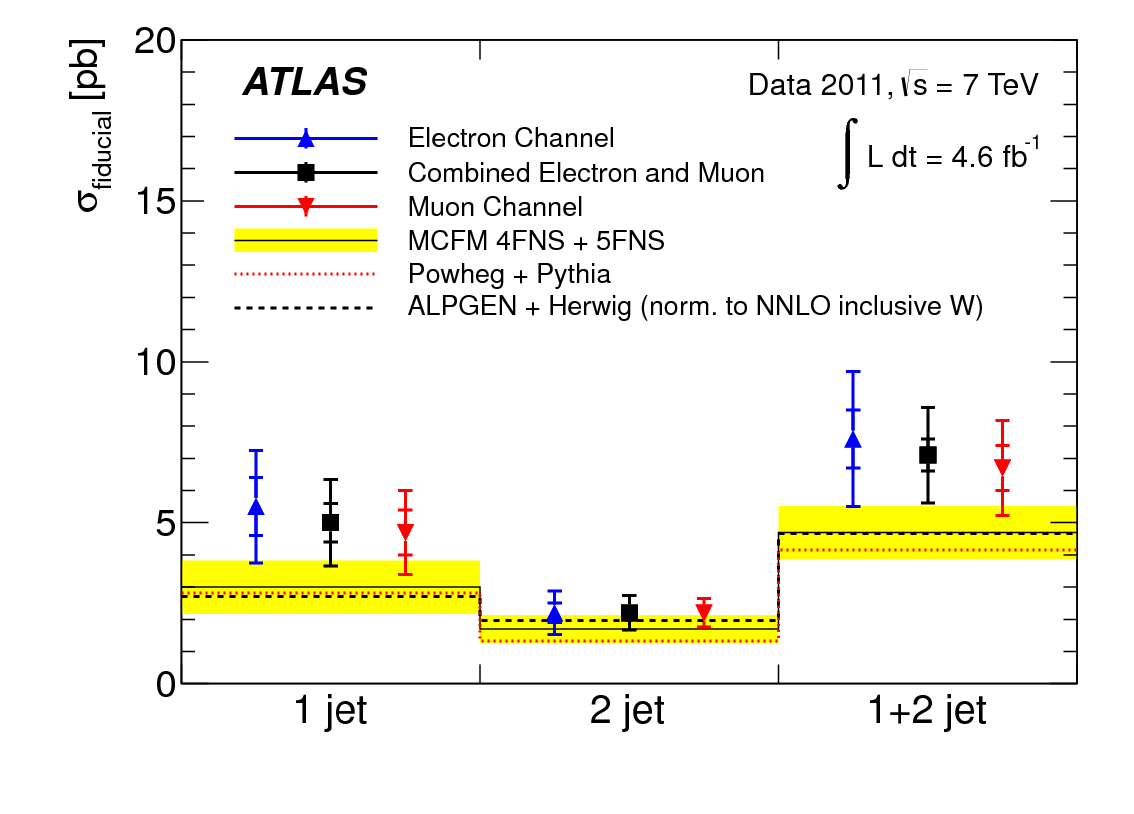
\includegraphics[width=0.5\textwidth]{images/ATLASWb.png}
  	\caption[ATLAS Wbb Results]
   	{ATLAS W+b cross section measurement at 7 TeV \cite{Aad:2013vka}}
	\label{fig:ATLASWb}
\end{figure}

By focusing on the observation of W-boson production with
two well-separated b-quark jets, this analysis provides an essential study to analyses where 
$\Wbb$ is an irreducible background
%in analyses involving two separated and well-identified b jets,
such as SM higgs boson production in association with
an electroweak gauge boson and subsequent decay to
$\bbbar$. %The discovery of a Higgs boson with a mass of approximately 125GeV
%by the ATLAS and CMS Collaborations~\cite{HiggsAtlas,HiggsCMS,LongHiggsCMS} motivates
%further studies to determine the coupling of this new boson to b quarks.

Other SM processes produce events with an experimental 
signature similar to the one studied here; these SM processes must be carefully
understood and modeled to obtain an accurate $\Wbb$ cross section measurement. 
These backgrounds include
production of top quark-antiquark pairs ($\ttbar$), associated production of a
$\PW$ boson with light jets misidentified as b-quark jets, single-top-quark
production, multijet production (henceforth labeled ``QCD multijet''), Drell--Yan production associated with jets, and electroweak diboson production.

The production mechanism of $\bbbar$ pairs together with
W or Z bosons has been the subject of extensive
theoretical studies and is included
in different simulation programs~\cite{Oleari:2011ey,Frederix:2011qg,Madgraph5} 
but is still not thoroughly understood.
According to the SM, the primary contribution for $\bbbar$ production in association with a W boson
is due to the splitting of a gluon into a $\bbbar$ pair.
Two different models for b-quark production are available, 
depending on whether there are four or five quark flavors
in the proton parton distribution functions (PDFs)~\cite{Compare4F5F}.

%Therefore, a precise experimental measurement of the $\Wbb$ production cross section
%provides important input to the refinement of theoretical calculations in
%perturbative quantum chromodynamics (QCD), as well as the validation of
%Monte Carlo (MC) techniques.

The analysis uses a sample of proton-proton collisions 
at a center-of-mass energy of $\sqrt{s}$=7 \TeV collected in 2011 with the CMS experiment at the LHC, 
corresponding to an 
integrated luminosity of $5.0\fbinv$.
%While the CMS detector is described in detail elsewhere~\cite{CMSExperiment}, the
%key components for this analysis are summarized here.
%The CMS experiment uses a right-handed coordinate system, with the
%origin at the nominal interaction point, the x-axis
%pointing to the center of the LHC ring, the y-axis pointing
%up (perpendicular to the plane of the LHC ring), and the z-axis
%along the counterclockwise-beam direction. The polar angle
%$\theta$ is measured from the positive z-axis and the
%azimuthal angle $\phi$ is measured in the x-y plane.
%The absolute value of the transverse
%momentum ($\pt$) is calculated as 
%$\pt = \sqrt{p_{\rm{x}}^2 + p_{\rm{y}}^2}$.
%%%%
%A superconducting solenoid occupies the
%central region of the CMS detector, providing an axial magnetic
%field of 3.8~T parallel to the beam direction.
%The silicon pixel and strip
%tracker, the crystal electromagnetic calorimeter, and the brass/scintillator hadron
%calorimeter are located within the solenoid. A quartz-fiber
%Cherenkov calorimeter extends the coverage to $|\eta| <$ 5.0, where pseudorapidity
%is defined as $\eta=-{\rm ln}[\tan{(\theta/2)}]$.
%Muons are measured in gas ionization detectors embedded 
%in the steel flux return yoke outside the solenoid.
%The first level of the CMS trigger system, composed of custom
%hardware processors, is designed to select the most interesting events
%in less than 3 $\mu$s using information from the calorimeters and muon
%detectors. 
%The high-level-trigger processor farm decreases the event rate from 100 kHz
%delivered by the first level trigger to a few hundred hertz, before data storage.

A number of Monte Carlo (MC) event generators are used 
to simulate the signal and backgrounds. 
The  events with W or Z boson production, or with 
$\ttbar$ production, are generated at leading order (LO) 
with \MADGRAPH 5.1~\cite{Madgraph5}, which is 
interfaced with \PYTHIA 6.4~\cite{Sjostrand:2006za} (also LO)
for hadronization.
Single top samples are generated at next-to-leading order (NLO) with 
\POWHEG2.0~\cite{Alioli:2008gx,Nason:2004rx,Frixione:2007vw}. 
Diboson ($\WW$, $\WZ$, $\ZZ$) and multijet samples are
generated with 
\PYTHIA 6.4~\cite{Sjostrand:2006za}. 
For LO generators, the default set of parton distribution functions
(PDF) used to produce these samples is CTEQ6L~\cite{CTEQ66}, while %describe this CTEQ6
MSTWNNLO~\cite{Martin:2009iq} is used for NLO generators. %describe mstwnnlo
For all processes, the detector response is simulated using a detailed
description of the CMS detector, based on the $\mathtt{GEANT4}$~
package~\cite{GEANT}, and event reconstruction is performed with
the same algorithms as used for data.
The simulated samples include additional interactions per bunch crossing (pileup),
the distribution for which comes from data.
Parton showering is simulated with PYTHIA using the Z2 tune~\cite{Field:2010bc}. %Describe Z2 Tune

%A complete reconstruction of the individual particles emerging from each collision event is obtained 
%via a particle-flow (PF) technique~\cite{CMS-PAS-PFT-09-001, CMS-PAS-PFT-10-002}. This 
%approach uses the information from all CMS sub-detectors to identify and 
%reconstruct individual particles in the collision event, classifying 
%them into mutually exclusive categories: charged hadrons, neutral hadrons, photons, electrons, and %muons.

A description of muon reconstruction  
 as well as a description of isolation is described in chapter \ref{chapter:EventReco}.
Muon candidates are required to be compatible with the primary vertex of the
event and have an isolation ($I^{\rm{rel}}$) less than 0.12. 
%, which is chosen as the vertex with highest $\sum \pt^2$ of its associated tracks.
%The muon relative isolation is defined as
%\begin{equation*}
%I^{\rm{rel}} = \left( \sum_{i}
%p_{\text{T, charged}}^i+ \sum_{j}  E_{\text{T, photon}}^j  +\sum_{k}  E_{\text{T, neutral}}^k \right) /\pt^{\mu},
%\end{equation*}
%with the sums running over all the charged and neutral PF candidates,
%excluding the muon candidate itself, 
%within a cone around the muon direction
%defined by  $\Delta R  < \Delta R_{\rm max} = 0.4$,
%where
%$\Delta R = \sqrt { (\Delta \eta)^2 + (\Delta \phi)^2 }$, and
%$E_{T}$ is 
%transverse energy.
Figure \ref{fig:muonvariables} shows the muon transverse momentum, pseudorapidity
and  Isolation ($I^\mathrm{rel}$) is shown in figure \ref{fig:qcdTemplate} (left).

\begin{figure}[b]
\centering
  \begin{subfigure}[b]{.45\textwidth}
	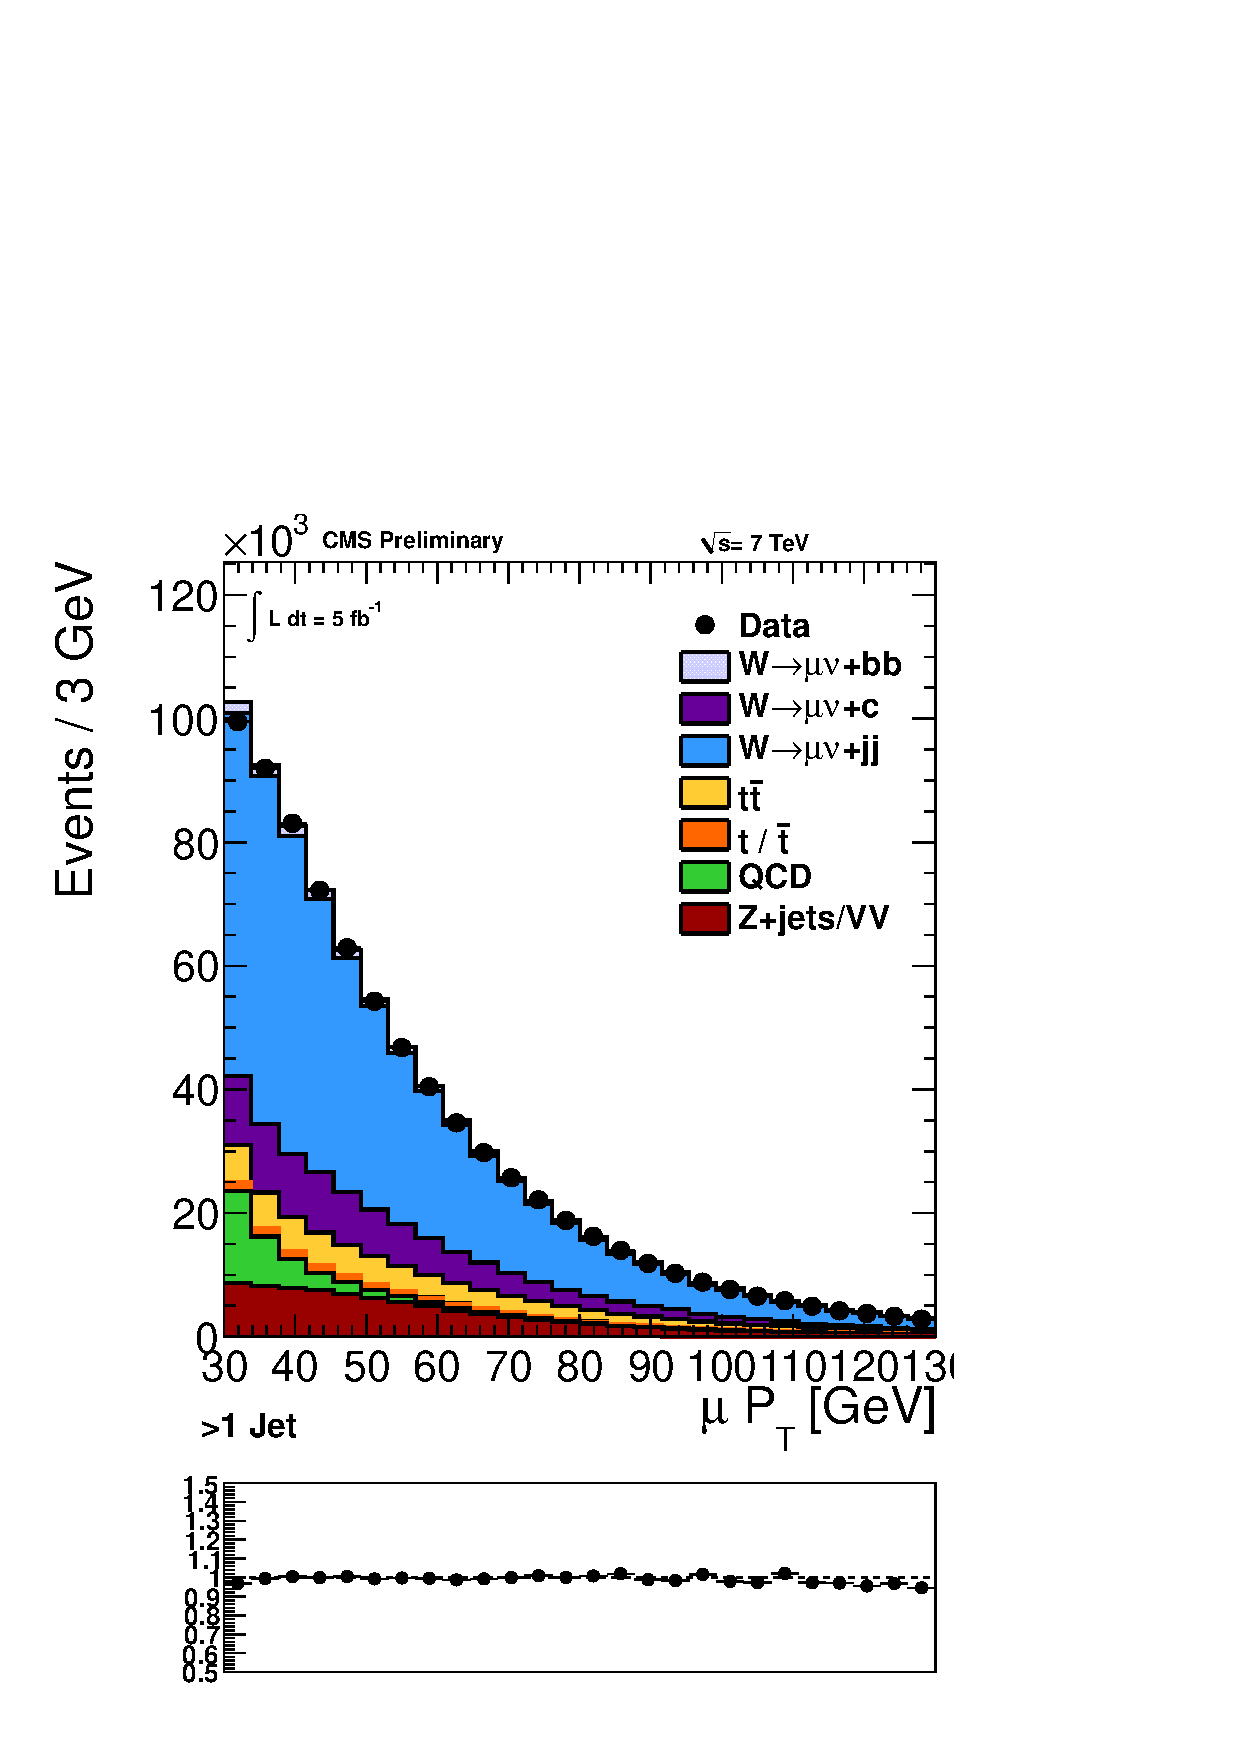
\includegraphics[trim = 0mm 52mm 0mm 0mm, clip,width=\textwidth]{images/muonPt.pdf}
	\caption[]{$\mu$    $p_{T}$ [GeV]}
	\end{subfigure}	
   \begin{subfigure}[b]{.45\textwidth}
	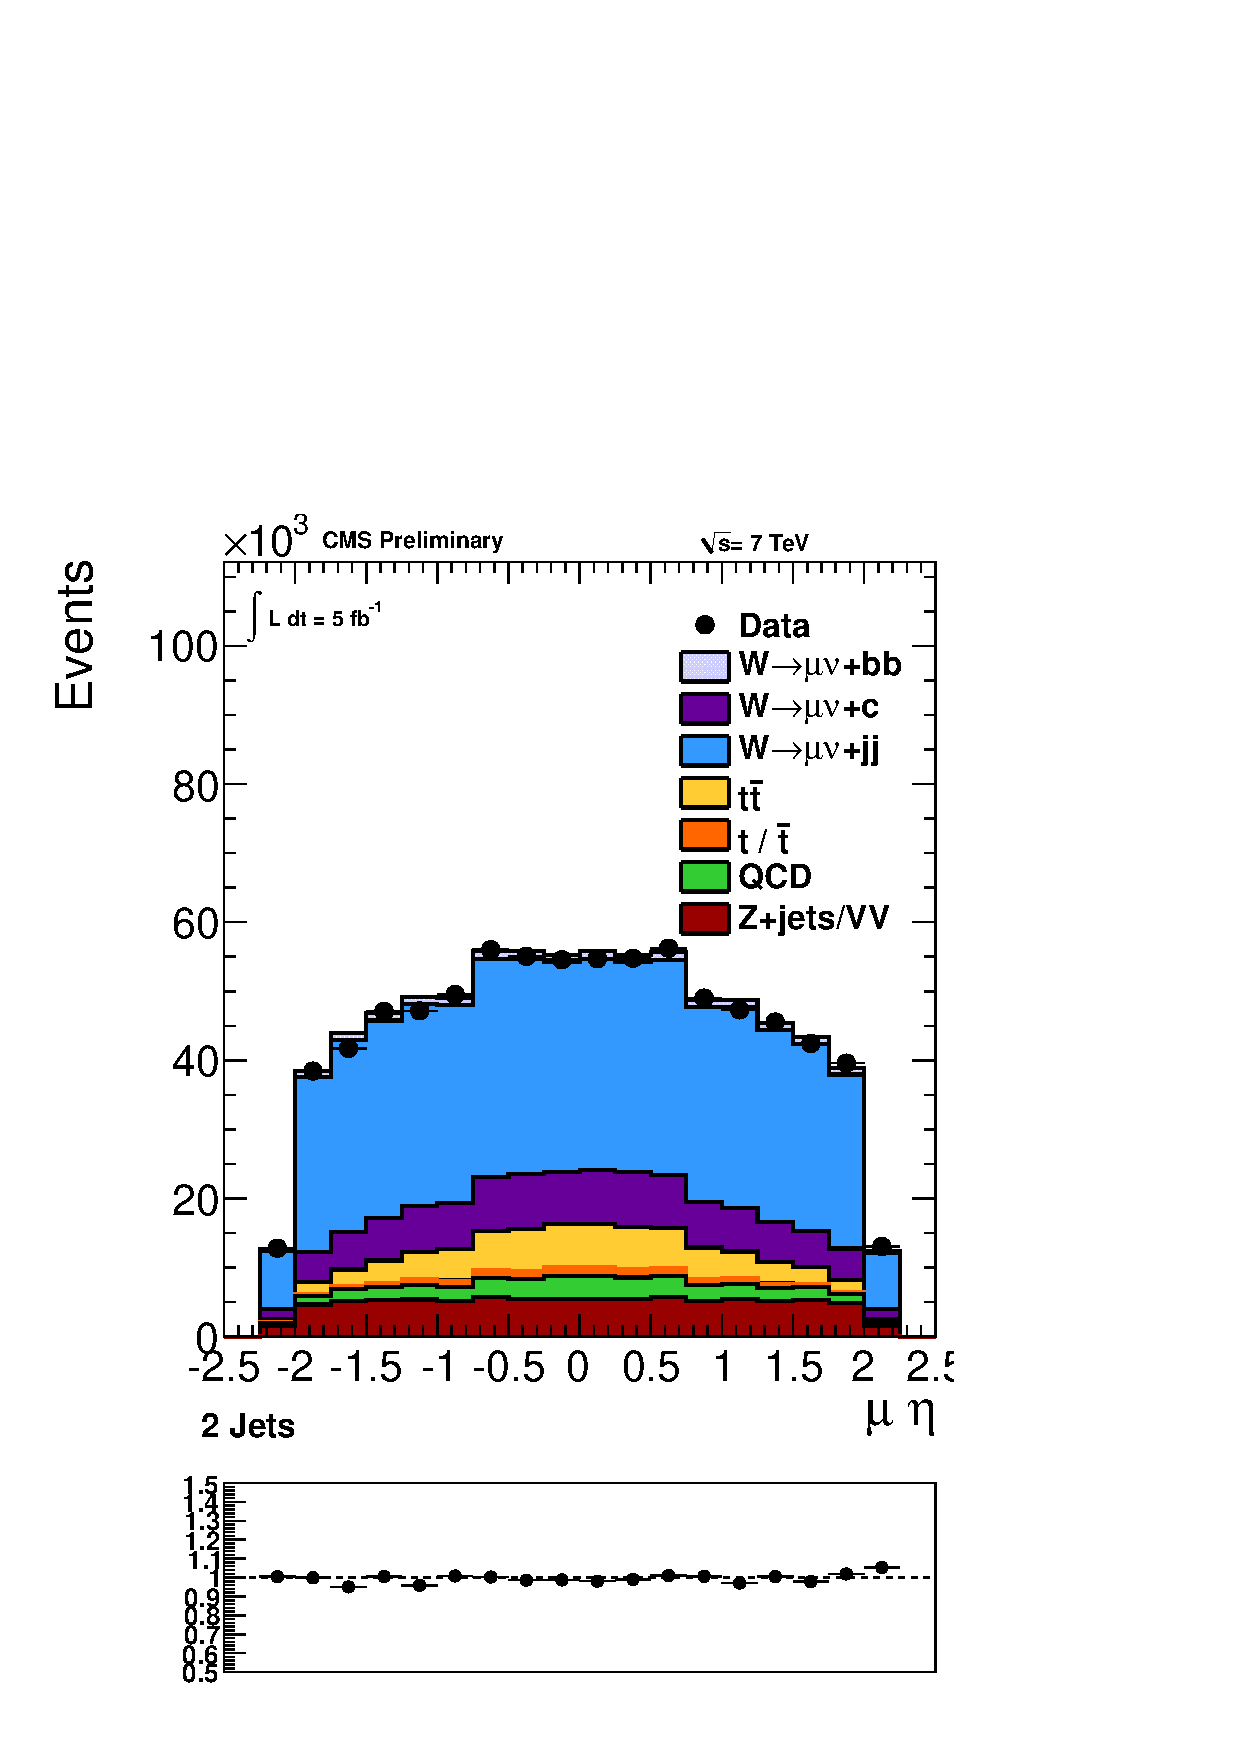
\includegraphics[trim = 0mm 52mm 0mm 0mm, clip,width=\textwidth]{images/muonEta.pdf}
	\caption[]{$\mu$    $\eta$}
    \end{subfigure}	
  \caption[]
   	{Muon $p_{T}$ and $\eta$ are shown above.}
    \label{fig:muonvariables}
\end{figure}

\begin{figure}[hb]
\centering
  \begin{subfigure}[b]{.45\textwidth}
	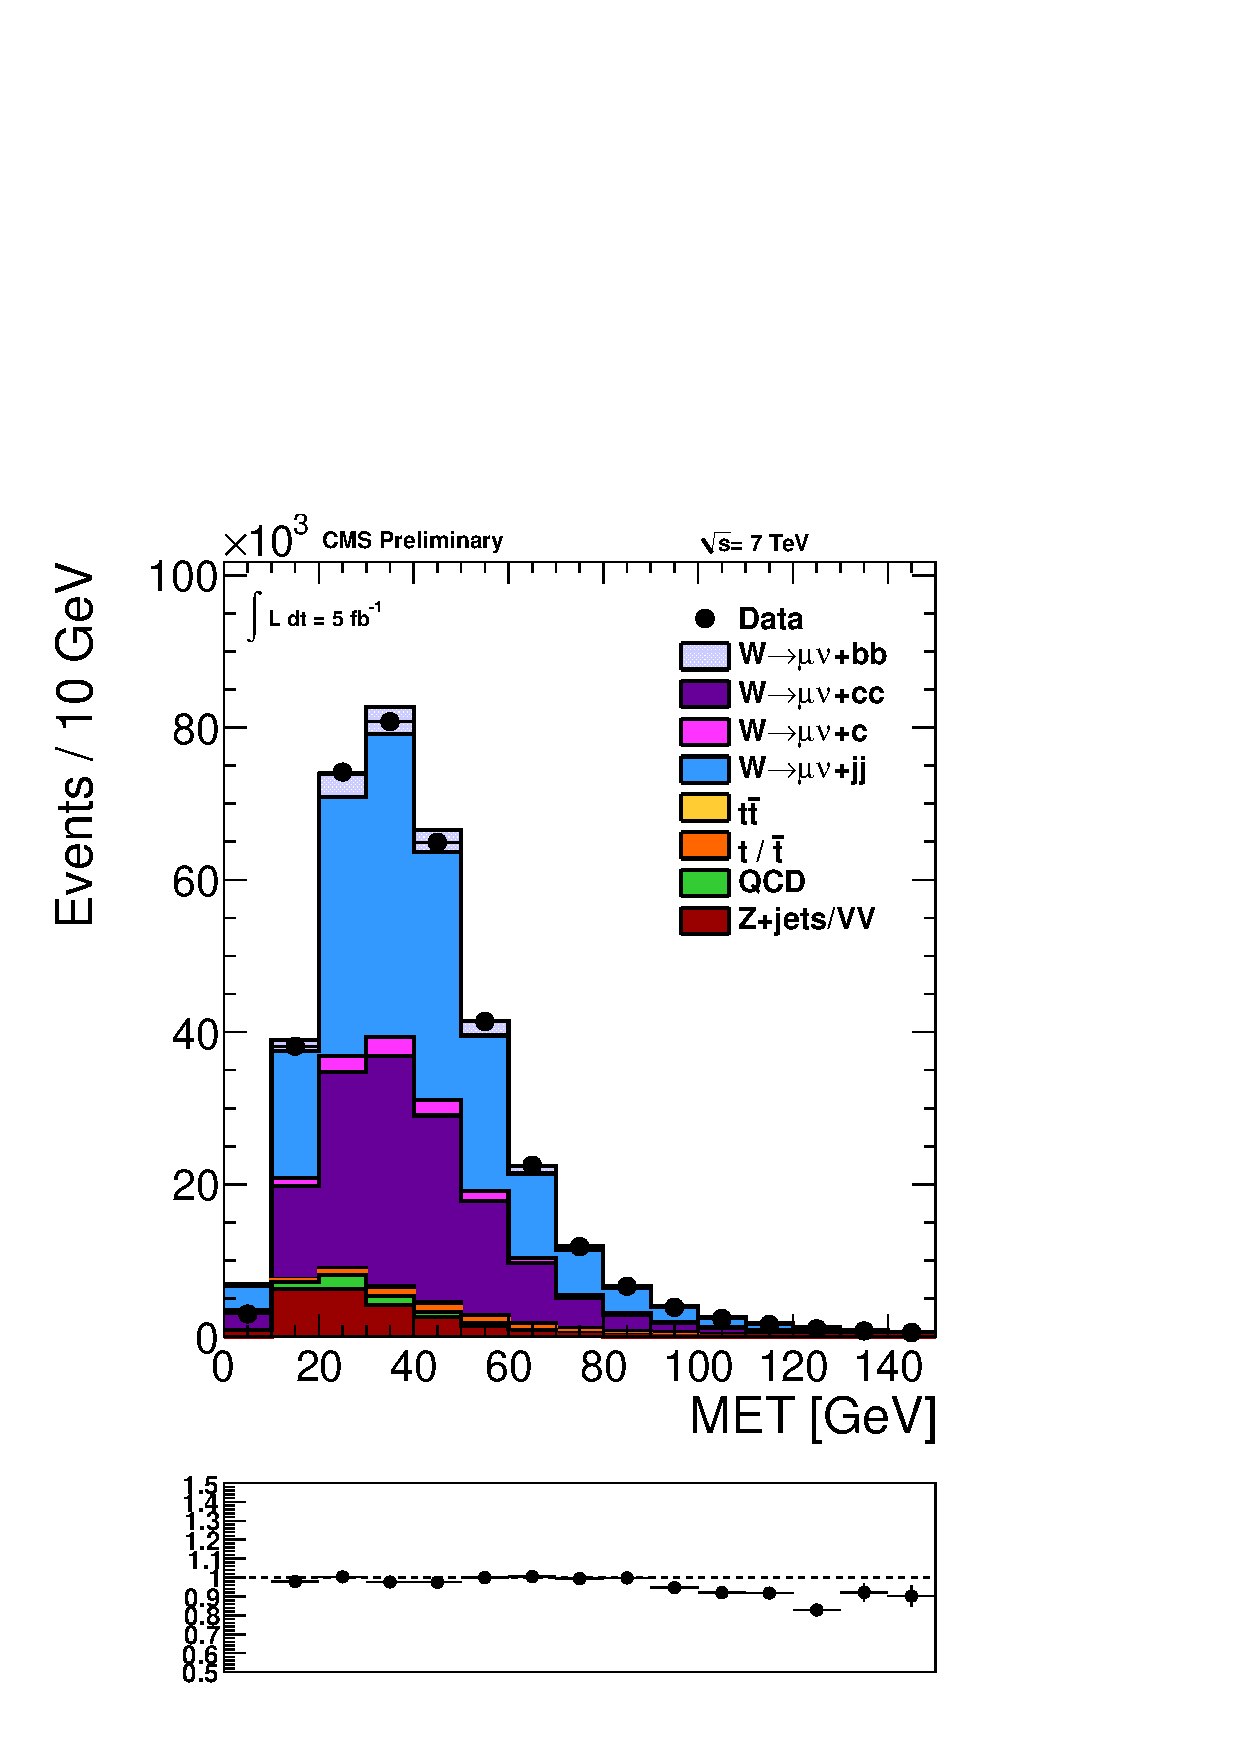
\includegraphics[trim = 0mm 52mm 0mm 0mm, clip,width=\textwidth]{images/met.pdf}
	\caption[]{$E_{T}^{miss}$ [GeV]}
	\end{subfigure}	
   \begin{subfigure}[b]{.45\textwidth}
	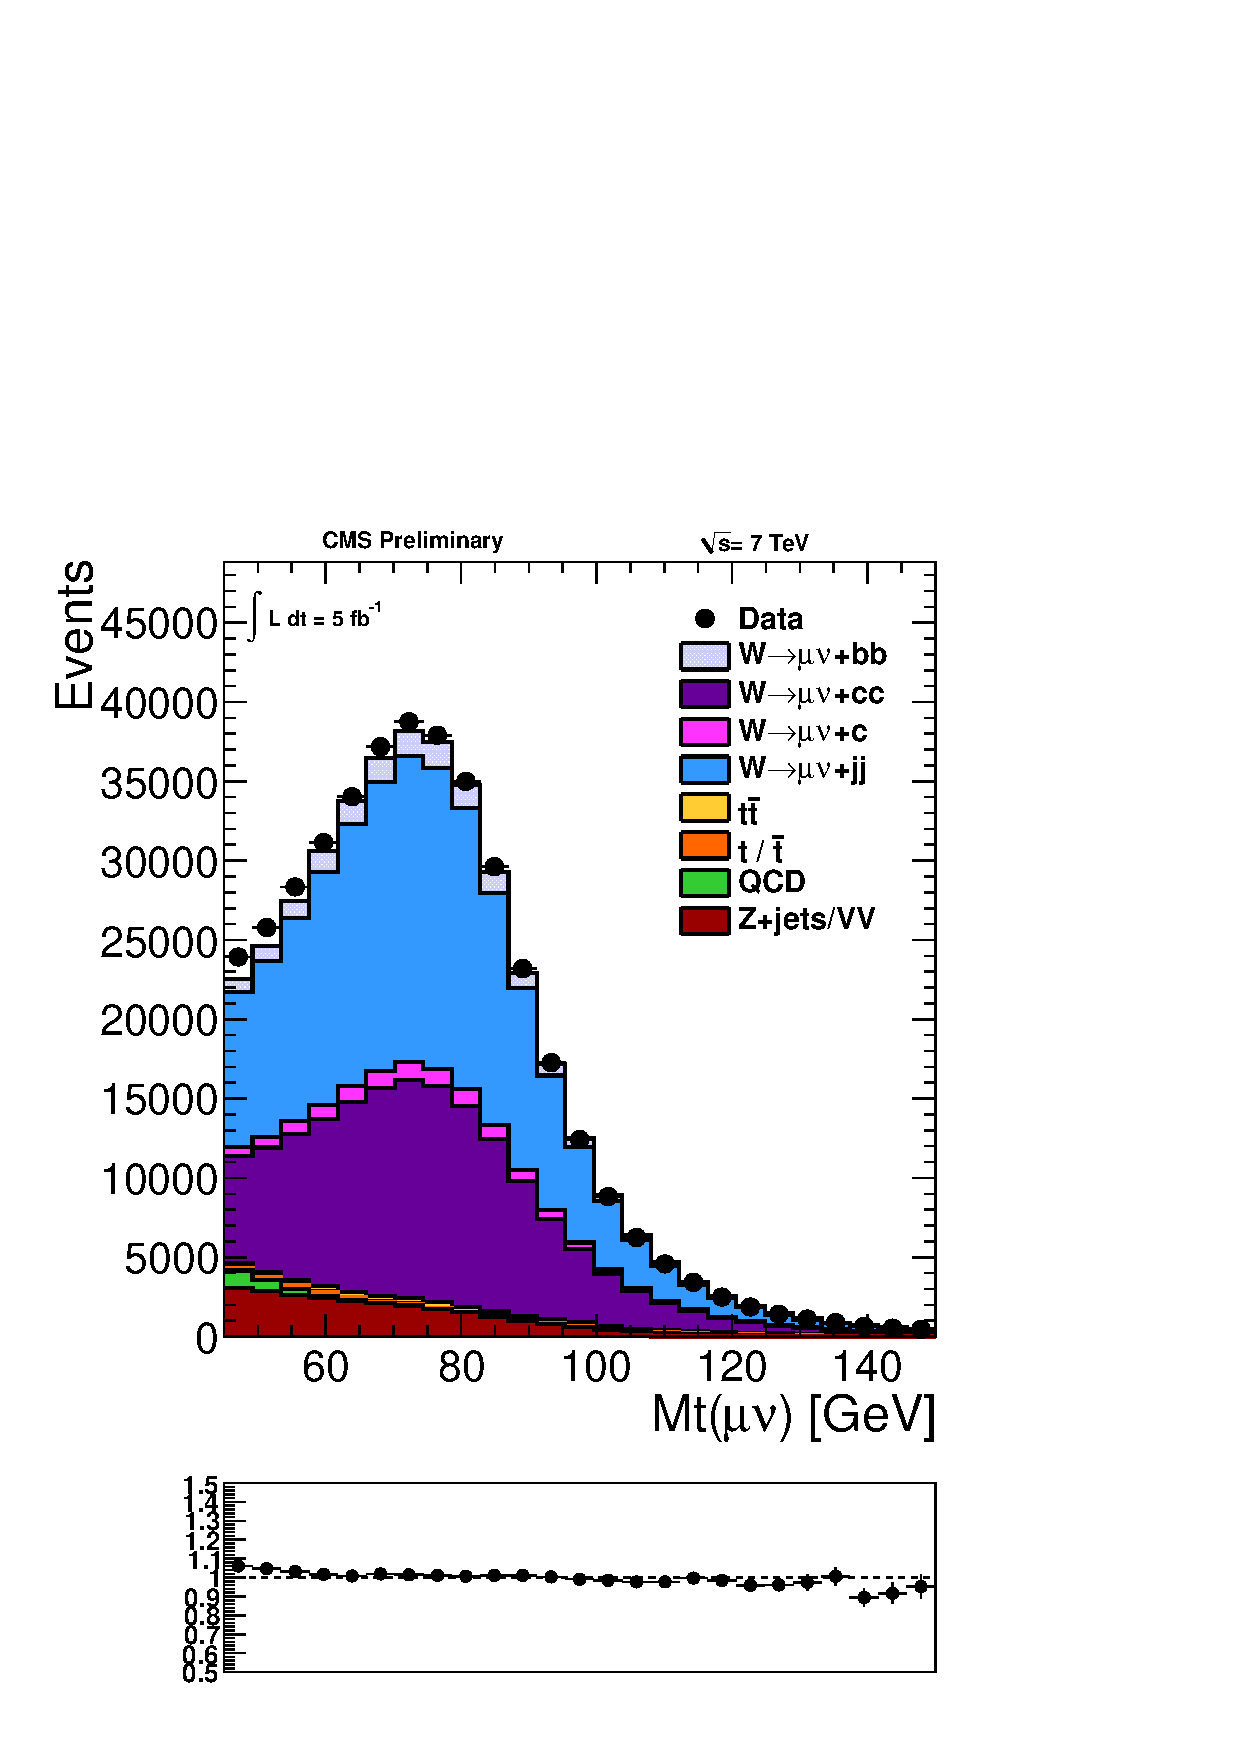
\includegraphics[trim = 0mm 52mm 0mm 0mm, clip,width=\textwidth]{images/MtCal.pdf}
	\caption[]{$M_{T}(\mu,E_{T}^{miss})$ [GeV]}
    \end{subfigure}	
  \caption[]
   	{The missing transverse energy ($E_{T}^{miss}$) and transverse momentum of muon and $E_{T}^{miss}$ ($M_{T}$) are shown above.}
    \label{fig:metVariables}
\end{figure}
%A muon isolation variable, $I^{\rm{rel}}$, is calculated as a 
%sum of the transverse energies  momenta of reconstructed PF particles in a 
%around the direction of the muon, normalized to the muon momentum,
%and excluding the contribution from the lepton candidate itself. 
%The muon is required to be isolated
%from any other detector activity according to the criterion $I^{rel}<0.12$. 

These identified, isolated muons are then combined with the missing transverse 
energy $\vecEtm$ of the event to form a leptonic W candidate. 
The missing transverse energy $\vecEtm$ is defined as
the negative vector sum of the
transverse momenta of all reconstructed particles in the event, with $\MET = |\vecEtm|$,
and is corrected using the procedure 
described in Ref.~\cite{WZCMS:2010}.
The reconstructed transverse mass of the system 
is built from the transverse momentum of the isolated muon 
and the missing transverse energy of the event, 
\begin{equation*} 
M_\mathrm{T} = \sqrt{2 \pt^{\ell} \MET (1-\cos \Delta \phi)}\ ,
\nonumber
\end{equation*}
where
$\Delta \phi$
is the difference in azimuth between $\vecEtm$ and $\vecPtmu$. In $\Wln$ decays the $M_T$ distribution presents a Jacobian peak 
with an edge at the W mass. Therefore it is a natural topological discriminator against non-W final states which yield a lepton candidate and
missing transverse energy, such as QCD multijet processes, 
in which the events concentrate at low values of the $M_T$ variable. The 
$M_\mathrm{T}$ and $M_{T}$ variables are shown in figure \ref{fig:metVariables}.

Jets are reconstructed from the PF candidates.
The anti-$\mathrm{k_T}$
clustering algorithm~\cite{Cacciari:2008gp} with distance parameter of 0.5
is used, as implemented in the \textsc{fastjet}
package~\cite{fastjet1,fastjet2}. Jet reconstruction 
is described in more detail in section \ref{sec:JetReco}.
Jets are required to pass identification
criteria that eliminate jets originating or being seeded by
noisy channels in the calorimeter~\cite{Chatrchyan:2009hy}.
In addition to this, jets originating from pileup interactions are
rejected by requiring compatibility of the jets 
with the primary interaction vertex. 
Jet energy corrections are also applied as a function of the jet
$\pt$ and $\eta$~\cite{cmsJEC}.

Secondary vertices (SV) are reconstructed inside each jet.
% using the trimmed kalman vertex 
%finder~\cite{XXX}.
This study makes use of the combined secondary vertex (CSV) b-tagging algorithm~\cite{refCSV};
this algorithm makes use of the
long lifetime and high mass of b hadrons
to provide optimized 
b-quark jet discrimination; 
the following variables are combined 
into a single discriminating variable using a likelihood ratio 
technique: secondary vertex mass, multiplicity of charged particles 
associated to the secondary vertex, the �ight 
signi�cance associated 
to the secondary vertex, the energy of charged particles associated 
to the SV divided by the energy of all charged particles associated to 
the jet, the rapidities of charged particle tracks associated to the 
secondary vertex, and the track impact parameter 
signi�cance 
exceeding the charm threshold.
If a jet does not have an SV then CSV algorithm computes 'pseudo Vertex' and 'No-Vertex' values.
%Through the use of a likelihood ratio technique jet identification variables 
%A single discriminator variable (known as a CSV discriminator) is created; 
Low values of the CSV discriminator mean the jet is less b jet-like, while values close
to 1 are more b jet-like. 
B-tagged jets are selected by imposing a 
minimum threshold on the CSV discriminator value.
The analysis is based on a CSV
discriminator threshold
which provides an efficiency of approximately 50$\%$  for identifying
jets containing b-flavored hadrons while reducing the 
misidentification probability for light-quark jets to 0.1$\%$~\cite{BTAGNOTE}
%%%% Note that TOP-12-024 quotes 45% - 0.1% 


\begin{figure}[t]
\centering
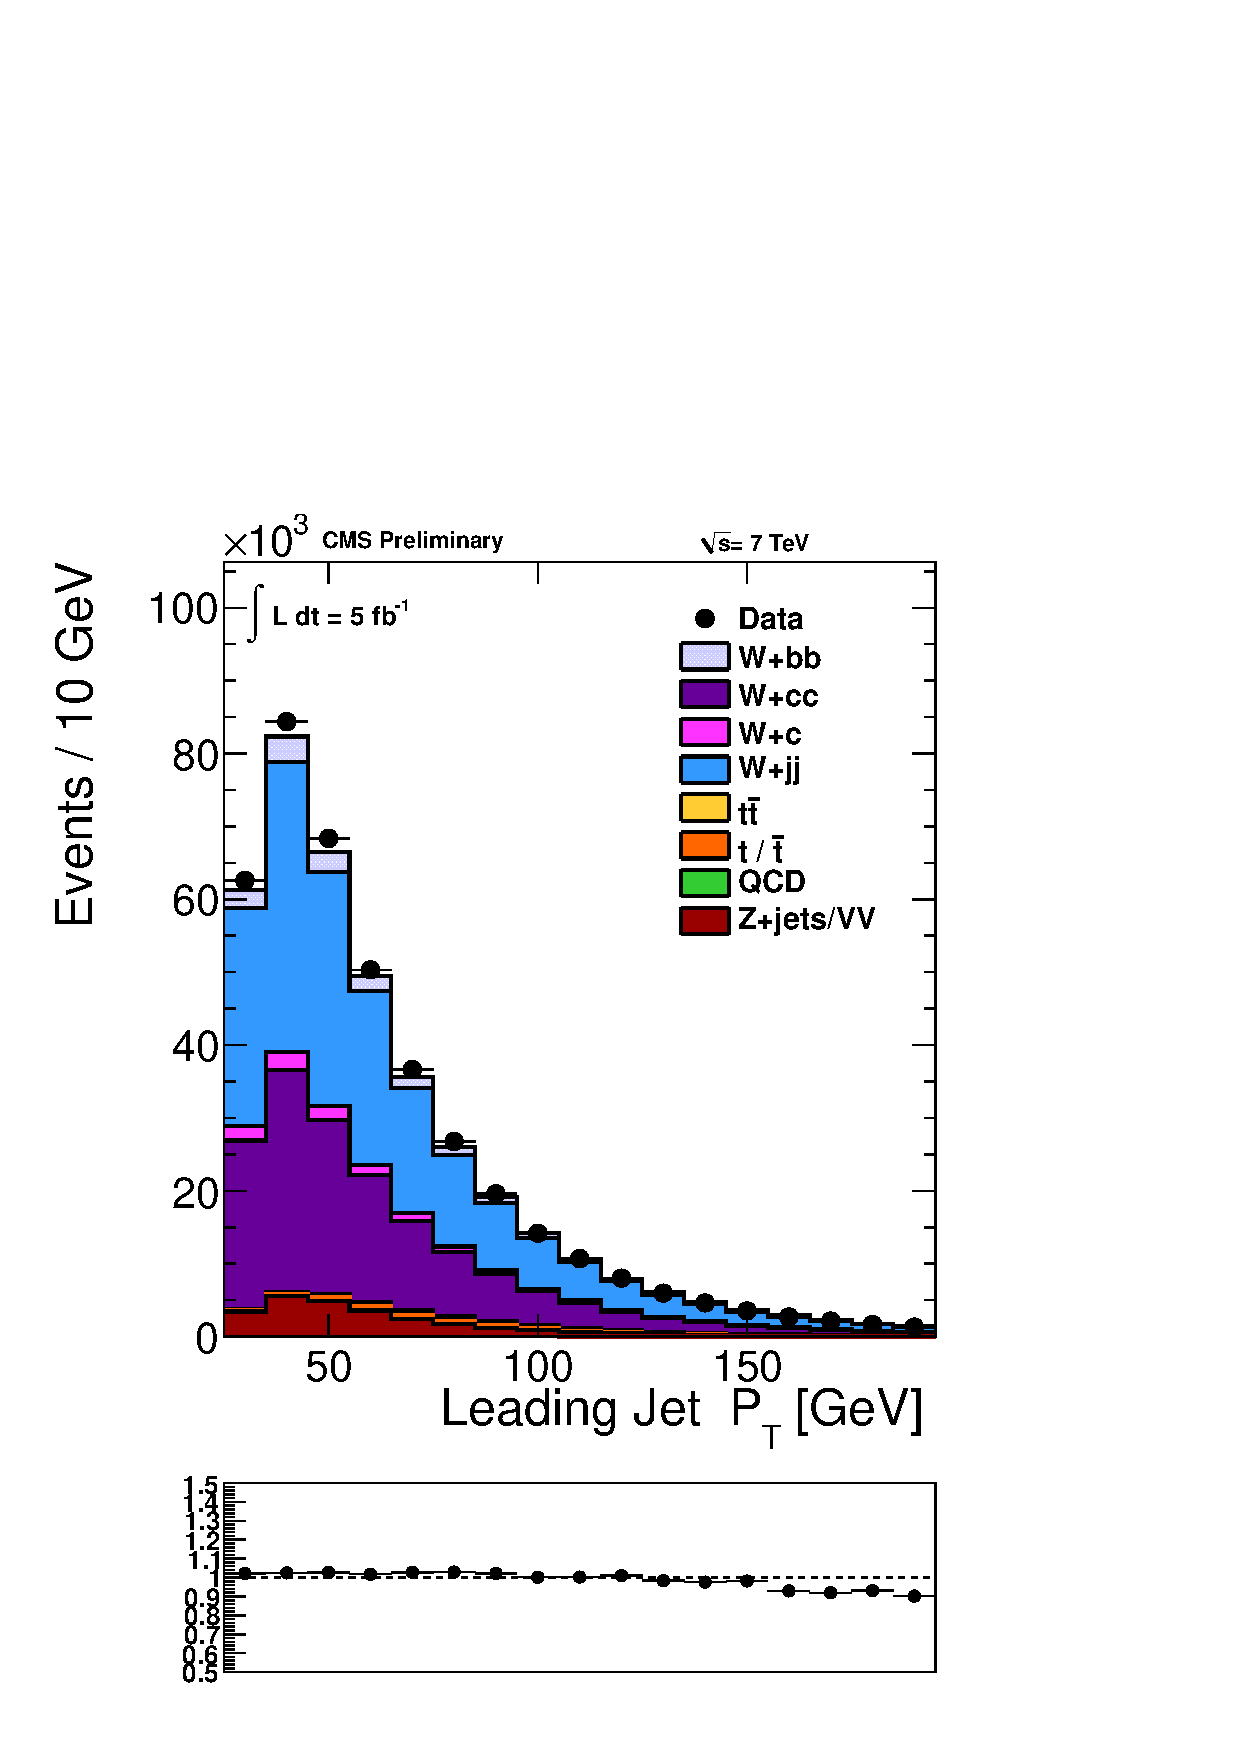
\includegraphics[width=0.45\textwidth, trim = 0 4cm 0 0, clip=true ]{Wbb/fig1.pdf}
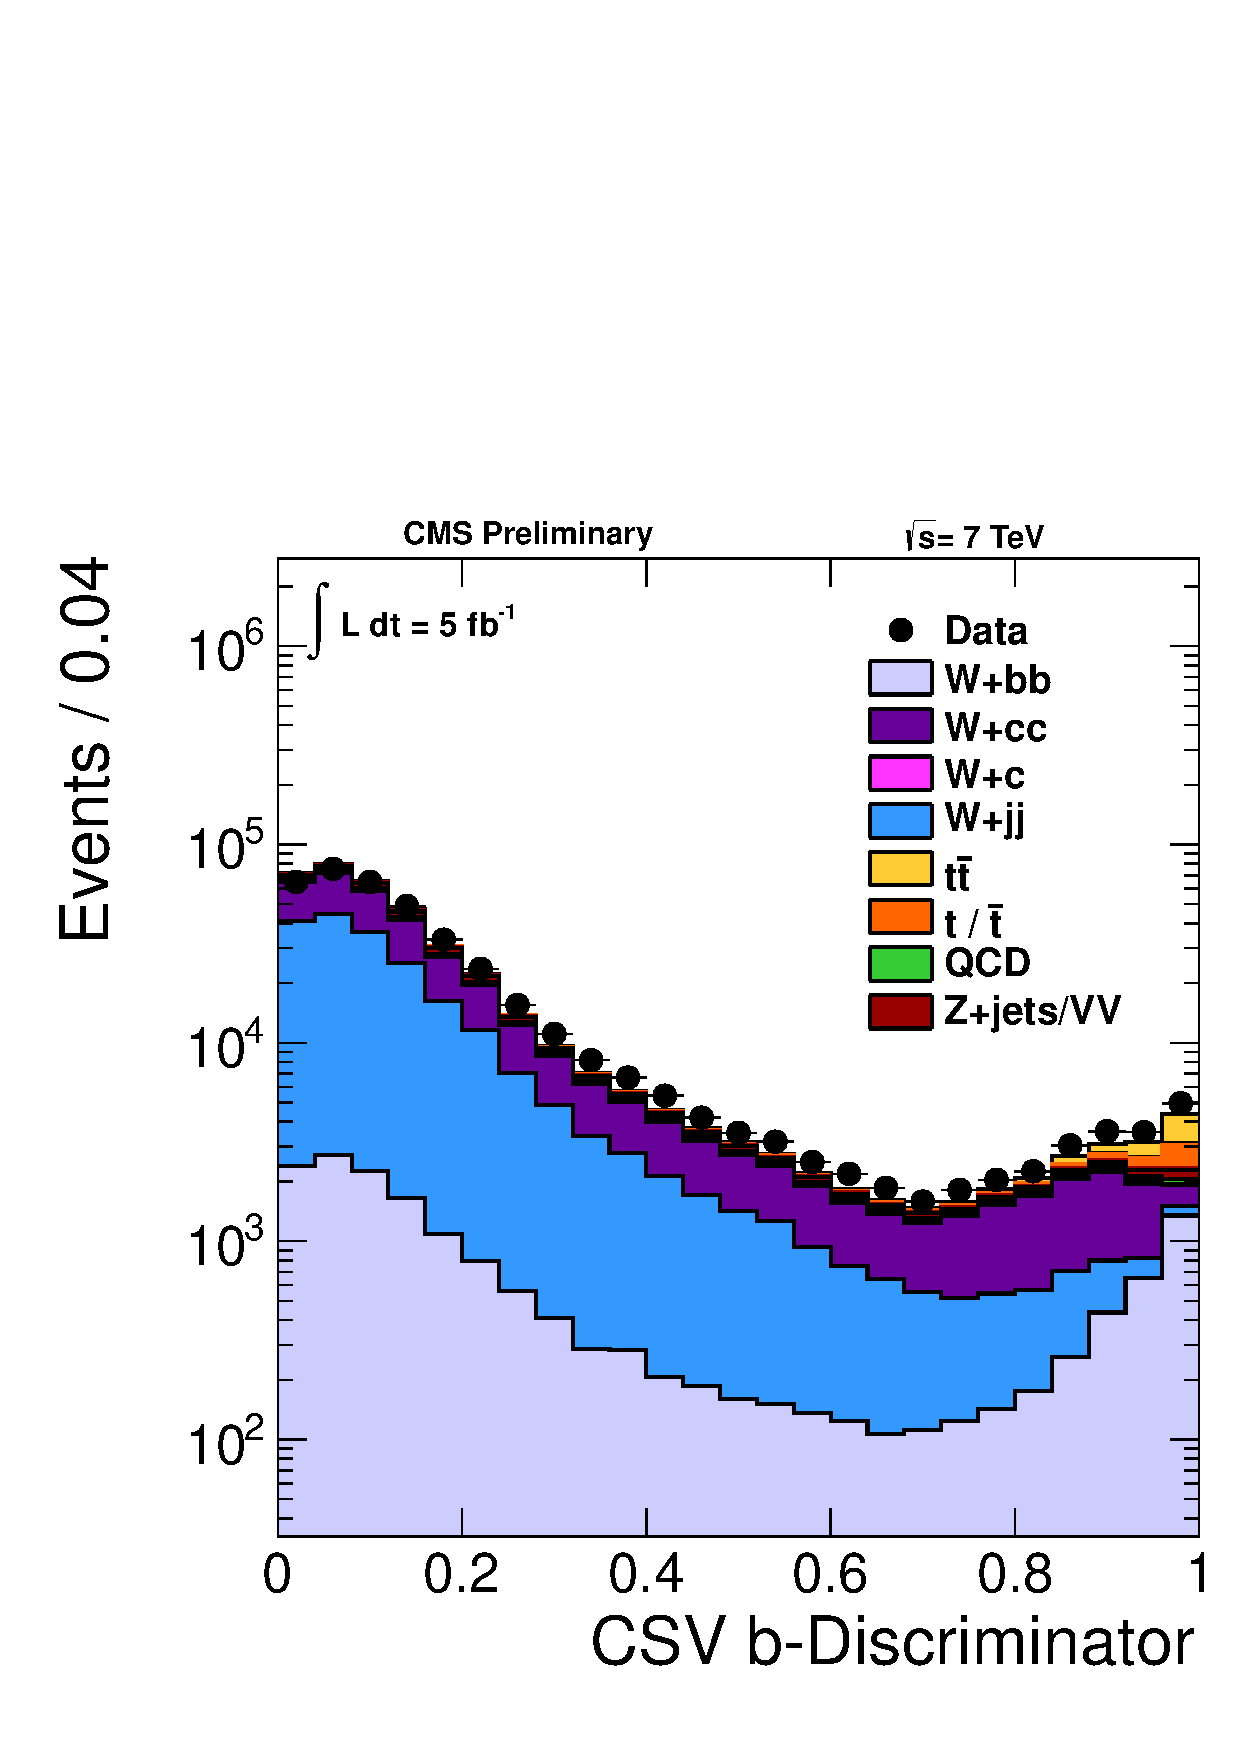
\includegraphics[width=0.45\textwidth]{Wbb/fig1_jetcsv.pdf}

\caption{(left) The highest-$p_{T}$ jet ($\rm{J_{1}}$) before applying b-tagging.
(right) The CSV b-discriminator 
for $\rm{J_{1}}$.}
\label{fig:figA}
\end{figure}


%The b-tagging working point
%chosen for the analysis is the tight one, in which the efficiency of the selection is approximately 60$\%$, 
%while a suppression
%factor for jets from light quarks is approximately 100~\cite{cmsBTAGPAPER}.

The $\Wbb$ selected events are required to have  
an isolated muon with $I^{\rm{rel}}<0.12$, $\pt>25GeV$, $|\eta|<2.1$,
exactly two jets with $\pt>25GeV$ and $|\eta|<2.4$, where 
both selected jets must contain a secondary vertex 
and pass the b-tagging CSV requirement.
To reduce the contribution from Z-boson production, the 
event is rejected if there is a second muon, without any requirements 
on the isolation and $\pt$, 
which builds with the isolated muon a dimuon system with 
invariant mass $m_{\mu\mu} > 60GeV$. 
The $\ttbar$ background is reduced by requiring
that there are no additional isolated electrons or muons with  $p_{T}>20GeV$ in the event and no
jets with $\pt>25GeV$ and $2.4<|\eta|<4.5$. To reduce the contribution
from QCD multijet events $\MT > 45GeV$ is also required. An evolution of the yields 
in monte carlo and data due to selection is shown in table (\ref{tab:eventsel1}).

\begin{table}[t]
\begin{adjustwidth}{-2.5cm}{}
\tiny
\begin{center}
%\footnotesize
\begin{tabular}{|c||c|c|c|c|c|c|c|c|c|c||c||c|}
\hline
Process &Wbb    &W+l      &W+c       &$\Wcc$  &Z+jets     &$t\bar{t}$ &Single-$t$  &VV    &QCD    &Total &Total \\
&&&&&&&&&&MC&Data\\
\hline
W+2jets & 39333.1& 378197.2& 23502.8 &284441.3 & 94169.7&74082.9&15880.3 &10195.0 &42276.7 &962079.0 &928445.0 \\
\hline
$M_{T}>45$ GeV & 30381.9& 291990.5& 18282.5 &221570.1 & 35144.1&54095.4&11909.0 &7780.7 &8393.9 &672138.2 &642674.0\\
\hline
JetVeto $\eta<2.4$& 21605.7& 237049.8& 14498.1 &175253.2 & 26490.8&9027.4&6599.4 &5744.0 &6520.0 &498028.4 &478315.0 \\
\hline
JetVeto $\eta<4.5$& 17152.9& 196618.2& 11853.4 &142711.5 & 21440.5&5390.2&4356.3 &4727.3 &5298 &405888.5 &408705.0\\
\hline
Lepton Veto & 17125.9& 196213.9& 11836.3 &142517.5 & 18994.8&4707.9&4155.8 &4446.5 &5284.3 &401973.7 &402742.0\\
\hline
\hline
2 CSV Tight Tags& 356.5& 47.3& 1.7 &56.3 & 34.5&620.6&168.0 &19.9 &36.3 &1249.3 &1387.0\\
\hline
$>$=1 SV    & 332.3& 1.5& 1.3 &21.0 & 30.9&595.5&160.3 &18.9 &33.1 &1194 &1230.0\\
in each jet & & $\pm 0.2$& $\pm 0.3$&$\pm4.3$ &$\pm 2.9$&$\pm 32.8$&$\pm 7.8$ &$\pm 0.8$ &$\pm 2.7$& $\pm 78.0$&$\pm 35.0$ \\
\hline
\hline
2 CSV Med Tags & 697.4& 227.2& 30.6 &340.8 & 83.4&1039.6&327.4 &42.3 &63.5 &2822.0 &3065.0\\
\hline
$>$= 1 SV& 557.5& 18.9& 12.7 &156.5 & 54.8&893.8&273.9 &33.1 &18.9 &2020.2 &2227.0\\
in each jet& & $\pm 1.9$& $\pm 1.3$& $\pm 31.2$&$\pm 5.4$&$\pm 53.6$&$\pm 14.5$ &$\pm 1.8$&$\pm 5.6$& $\pm 153.3$&$\pm 47.2$ \\
\hline
\end{tabular}
\caption{Evolution of event selection}
\label{tab:eventsel1}
\end{center}
\end{adjustwidth}
\end{table}

After all the selection requirements the significant background 
contributions are:
$\ttbar$, single top, W+jets (u,d,c,s,g), Z+jets (u,d,c,s,b,g) and QCD multijet. 
Final contributions of these backgrounds in the signal region are computed via  
a simultaneous fit. This fit is described in section \ref{sec:finalfit}
and provides the final estimate for the signal and background yields.
The initial yields are taken either from data, in estimates based on the 
control regions, or from simulation, normalized to the NNLO predictions.
The shapes and normalizations of the background distributions
are validated in data with a set of control regions, as described in the next sections.

\subsection{QCD multijet background}
With the exception of QCD, the shapes of the background distributions are taken from simulation. 
A shape for the QCD template is obtained directly from  
a multijet-enriched control region in data. 
To create a control region enriched in QCD events all selection requirements, including lepton and jet
vetos, are applied, except the isolation requirements of the main lepton are inverted. The muon is
required to have $I_{rel}>0.2$; figure \ref{fig:muonvariables} shows the muon isolation distribution. Good agreement between data and monte carlo is observed. 
 After selecting these non-isolated events, there remains a significant
number of top, W and Z events estimated from MC simulation.
These events make up to approximately 10$\%$ of all events in the control region and
are subtracted from data
to construct the QCD shape in the signal region; 
this background subtraction is illustrated in Fig.~\ref{fig:qcdTemplate}.
The initial normalization of the QCD yield (before final signal extraction) is found 
by performing a fit in the $M_{T}(W)$ distribution in the region where $M_{T}(W)<45$.
The QCD uncertainty in the 
final fit is taken to be $\pm$50\%. This uncertainty is sufficient to provide coverage for 
normalization and shape mismodelings of the small QCD contribution in the final selection.

\begin{figure}[t]
      \center
             \begin{subfigure}[b]{.47\textwidth}
	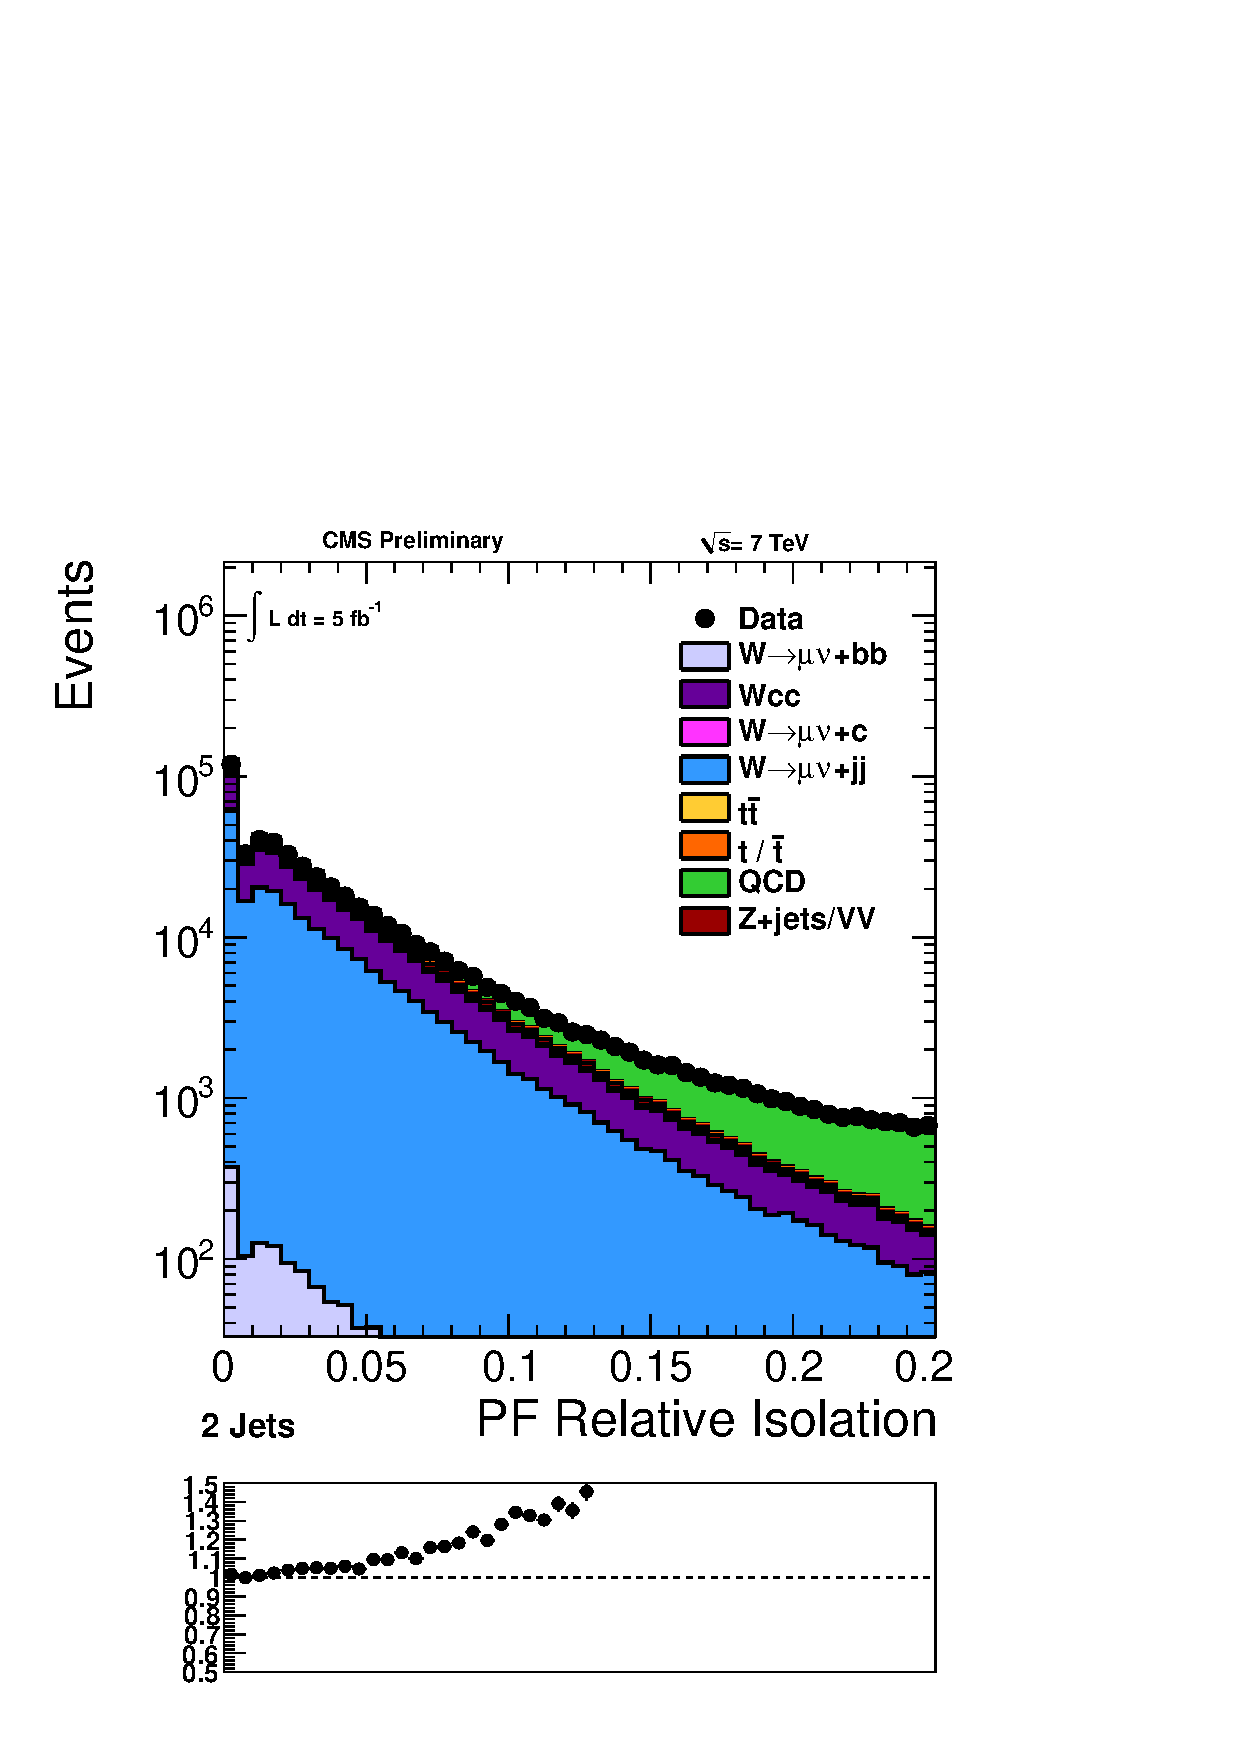
\includegraphics[height=6.5cm, trim = 0mm 52mm 0mm 0mm, clip,width=\textwidth]{images/muNuRelPFIso.pdf}
	\caption[]{$\mu$    $I^{\mathrm{rel}}$}
    \end{subfigure}
       \begin{subfigure}[b]{.47\textwidth}
      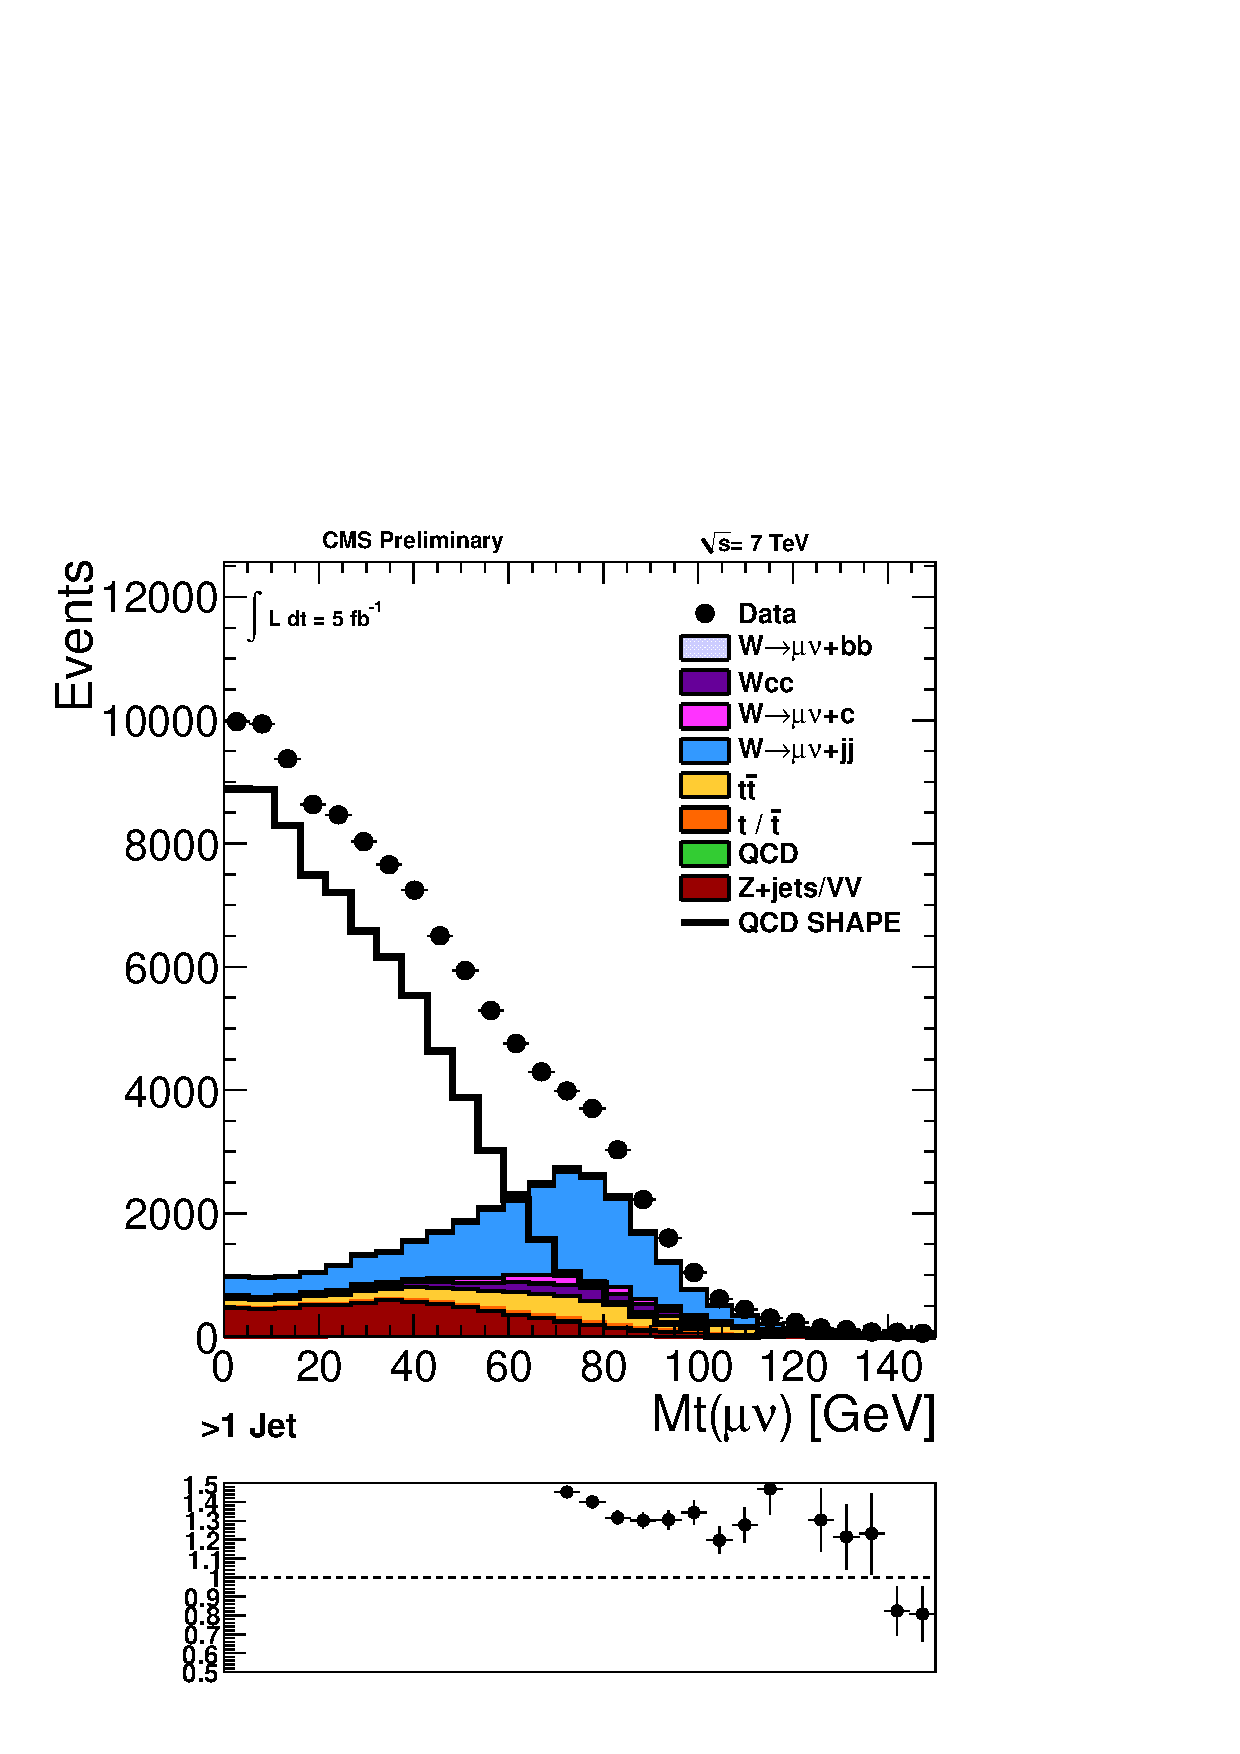
\includegraphics[height=6.5cm, trim = 0 5.2cm 0 0, clip=true, width=\textwidth]{Wbb/MtCal_Iso.pdf}
\caption[]{$M_{T}$    [GeV]}
    \end{subfigure}
      \caption{Muon Isolation (left). The contributions of individual backgrounds in the
      anti-isolated $M_{T}$ distribution (right).
      The template for the QCD shape is taken as the difference between simulation 
      and data in the non-isolated region.}
      \label{fig:qcdTemplate}
\end{figure}

\subsection{W+jets: light and charm component}
The W+$\rm{jets}$ (u,d,c,s,g) process, where the jets are not initiated by b quarks,
is the dominant background before applying the selection requirements on the secondary vertex and
b-tagging. Figure~\ref{fig:figA} (left) shows the $\pt$ of the leading jet at 
this preselected stage. The CSV algorithm working point which provides maximum reduction of 
W+$\rm{jets}$ (u,d,c,s,g) is used. 
The CSV b-tagging discriminant for the leading jet is shown in 
Figure~\ref{fig:figA} (right). 

The presence of light and charm jets
in the sample is very small at the higher values of the discriminant.
Furthermore, to increase the purity of the sample 
%maximally reduce the contribution from the $\Wcc$ process 
a secondary vertex is required to be reconstructed in each of the selected jets.
Figure~\ref{fig:figAbis} shows the mass of the secondary vertex of the 
leading jet ($\rm{J_{1}}$, right) and the sub-leading jet ($\rm{J_{2}}$, left), for the final selection
in the signal region.
These selection requirements have been validated in the $\ttbar$ and Z+jets control regions
described below. 
%in the $\cPZ$+bb and $\ttbar$ control regions. 
%The number of secondary vertices before b-tagging for the signal region region is plotted in Figure~\ref{fig:fig}.

\begin{figure}[b]
    \center
    \subfloat{\label{fig:WBB_J1_J2_SVMass}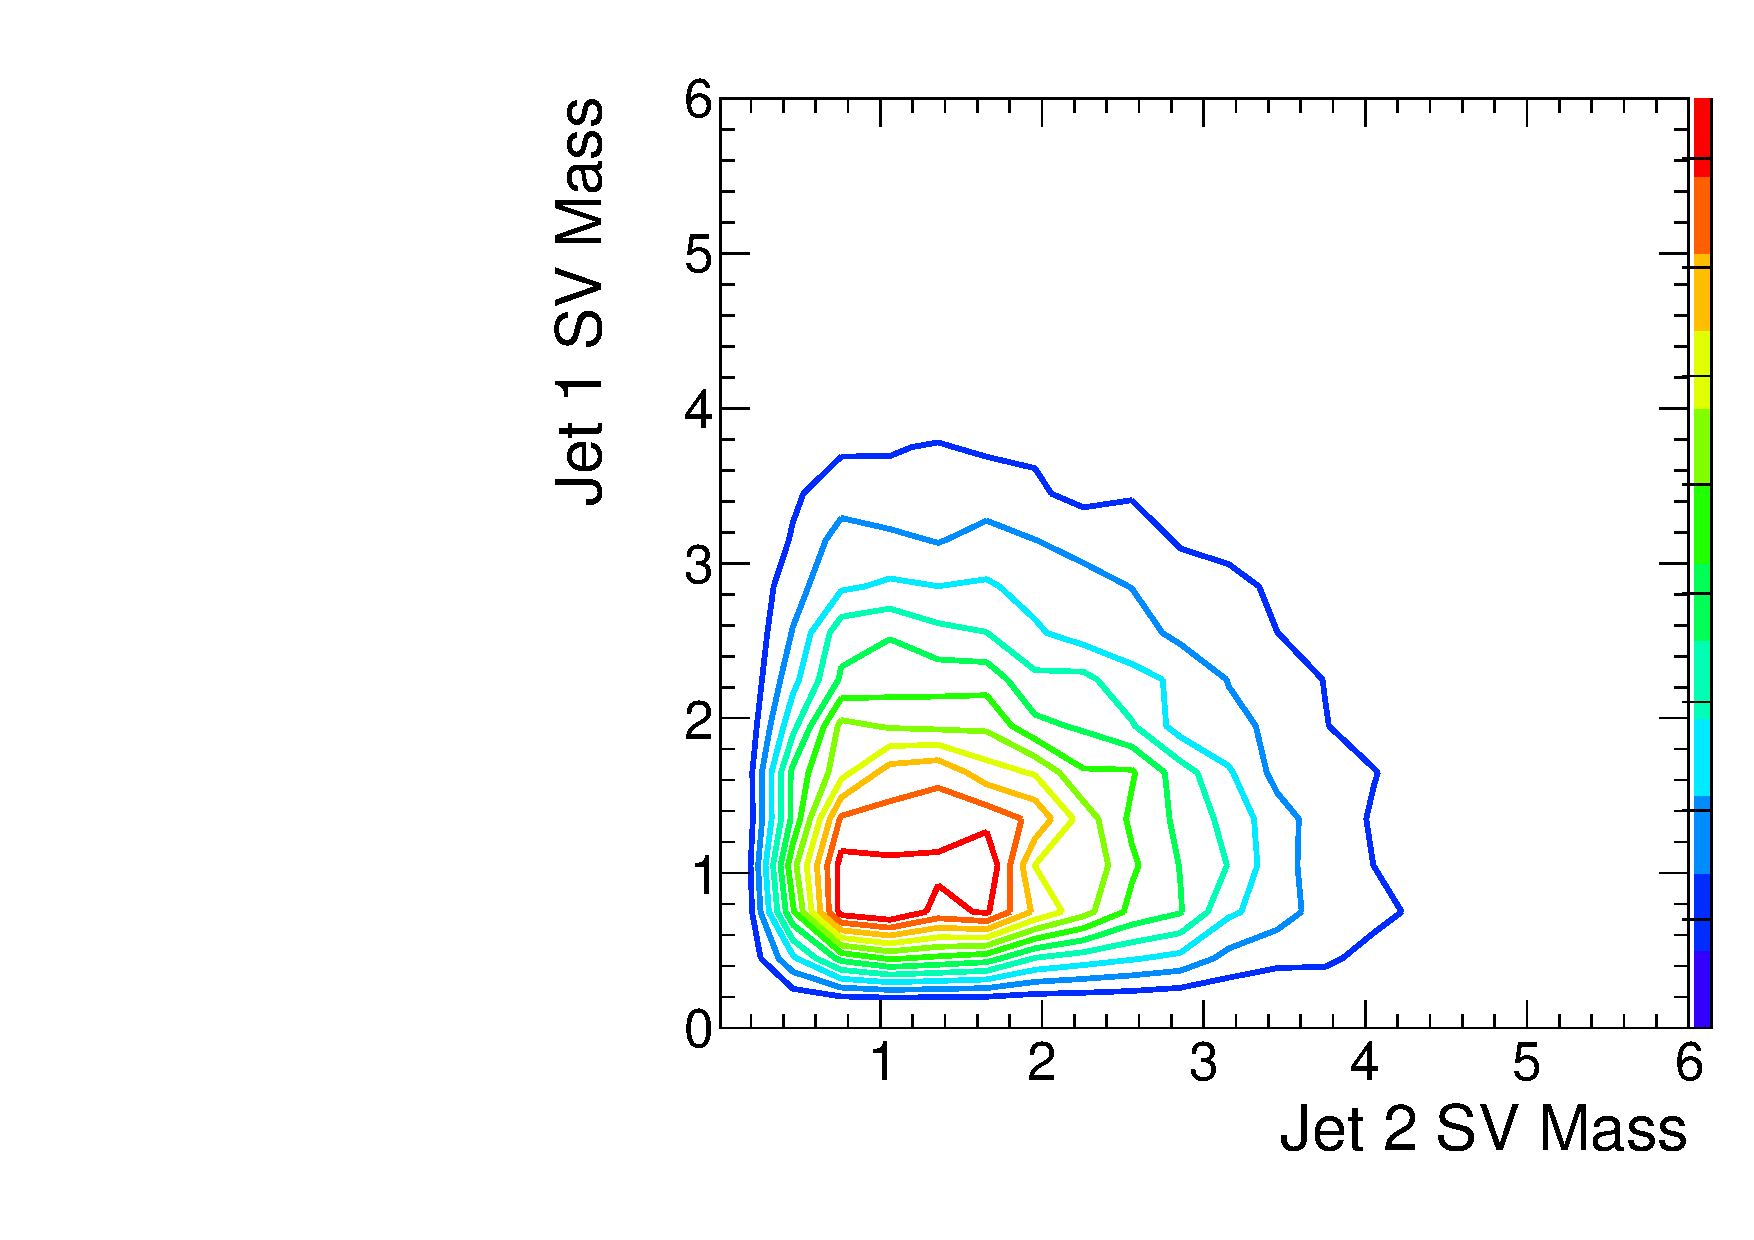
\includegraphics[height=7cm]{Wbb/WBB_J1_J2_SVMass.pdf}}
    \subfloat{\label{fig:WC_J1_J2_SVMass}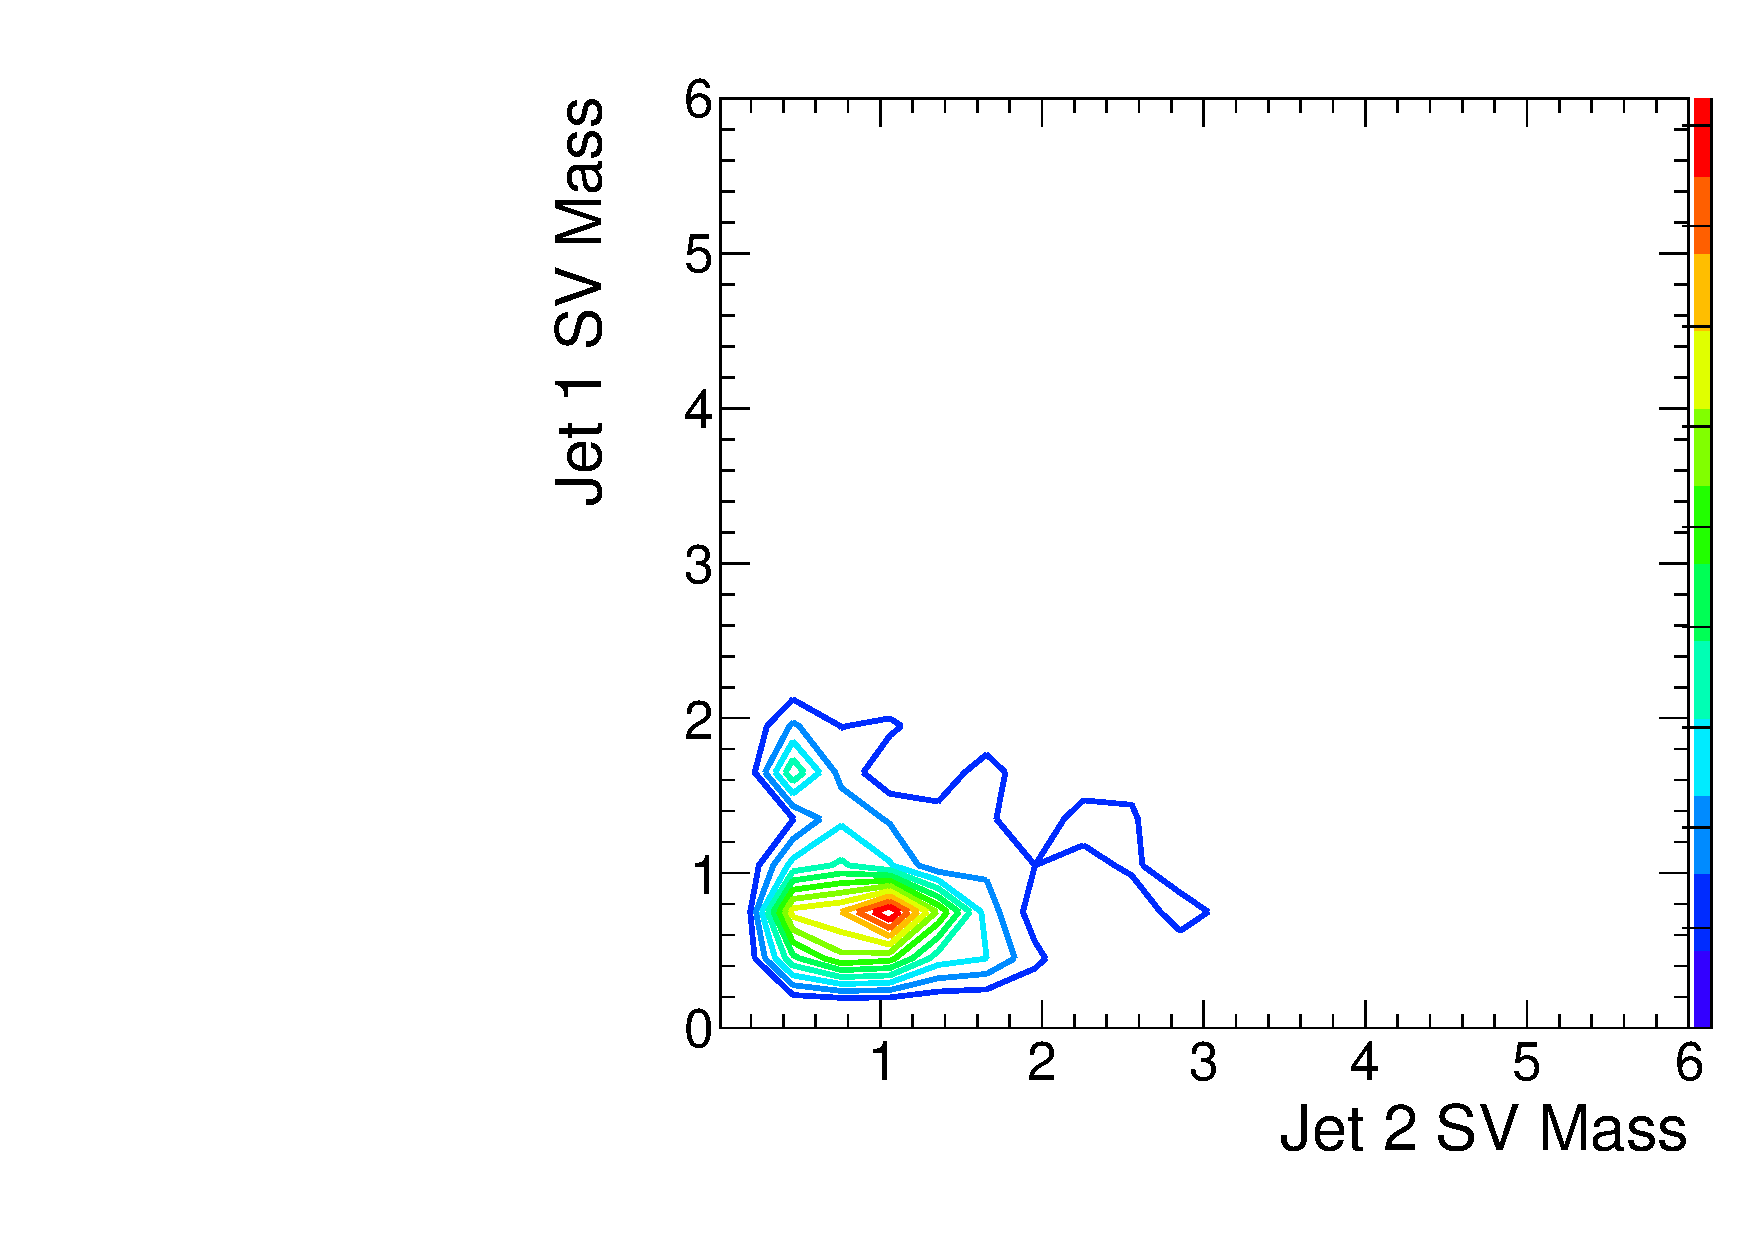
\includegraphics[height=7cm]{Wbb/WC_J1_J2_SVMass.pdf}}
    \caption{Contour plot high $p_{T}$ vs. second highest $p_{T}$ secondary vertex mass. 
    The W+c secondary vertex mass is concentrated in the 
    region where the secondary vertex masses of the jets sum is less than 3.
   \label{fig:SVMassContourShapes}
      }
\end{figure}

A powerful discrimination variable to distinguish $\Wbb$ and $\Wcc$ is
the sum of the masses of the two secondary vertices 
('J1SVMass + J2SVMass') corresponding to the two b jets.
The correlation between J1SVMass + J2SVMass is shown in 
Figure \ref{fig:SVMassContourShapes} for the
$\Wbb$ and $\Wcc$ samples. It is clear from this distribution 
that $\Wbb$ populates the high mass region
of the phase-space (J1SVMass + J2SVMass$\>$3 GeV) 
while the $\Wcc$ contribution populates the low mass region of the
phase-space.
This distribution is shown in figure~\ref{fig:figC} for 
jets passing the CSV medium working point.

%\begin{figure}[t]
%    \center
%    \subfloat[]{\label{fig:AddMassCSVM}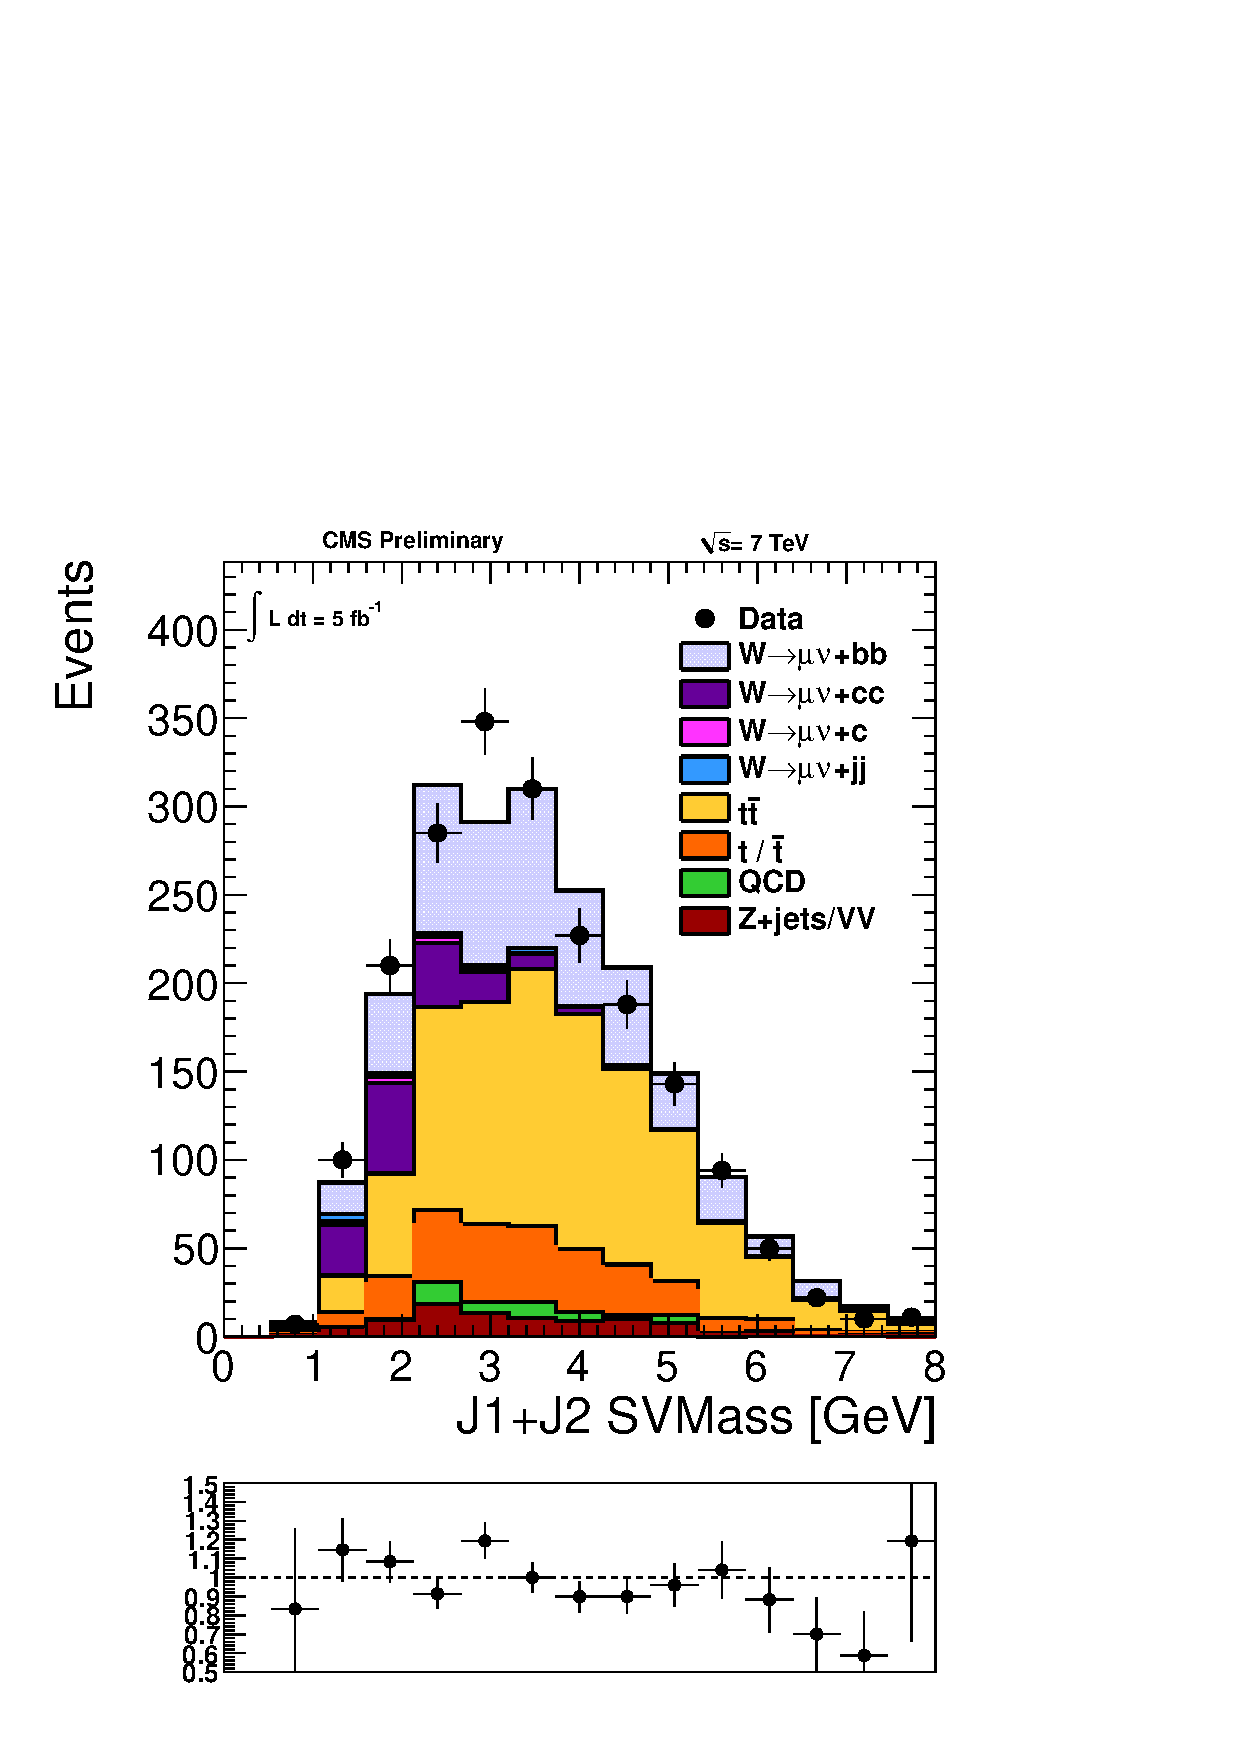
\includegraphics[height=7.5cm]{Wbb/AddSVMassM.pdf}}
%    \subfloat[]{\label{fig:AddMassCSVT}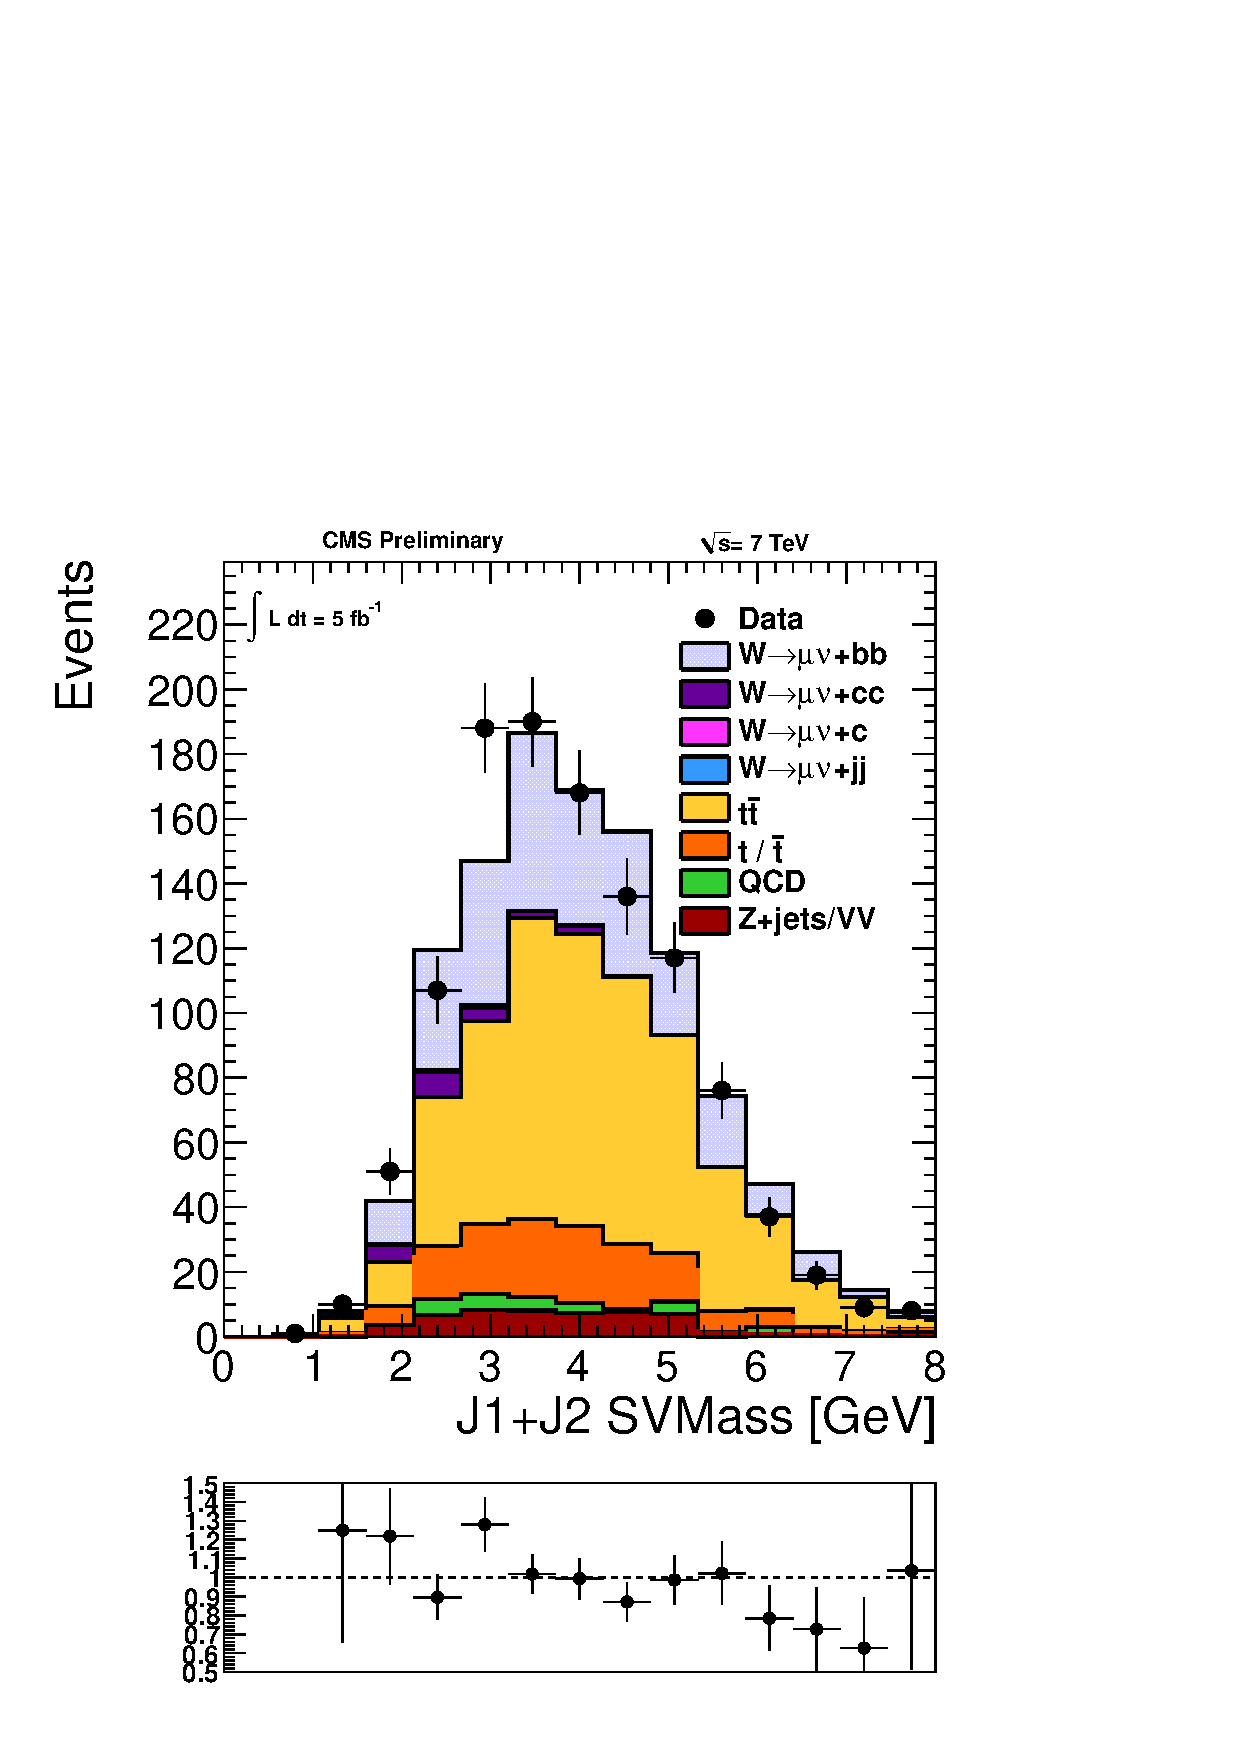
\includegraphics[height=7.5cm]{Wbb/AddSVMassT.pdf}}
%    \caption{Sum of masses the secondary vertices ('J1SVMass + J2SVMass'), for events with two jets
%      passing the medium (\ref{fig:AddMassCSVM}) or tight (\ref{fig:AddMassCSVT}) CSV working points.}
%    \label{fig:SVMASS_2WPS}
  %\end{center}                                                                                                                            
%\end{figure}

\begin{figure}[t]
\centering
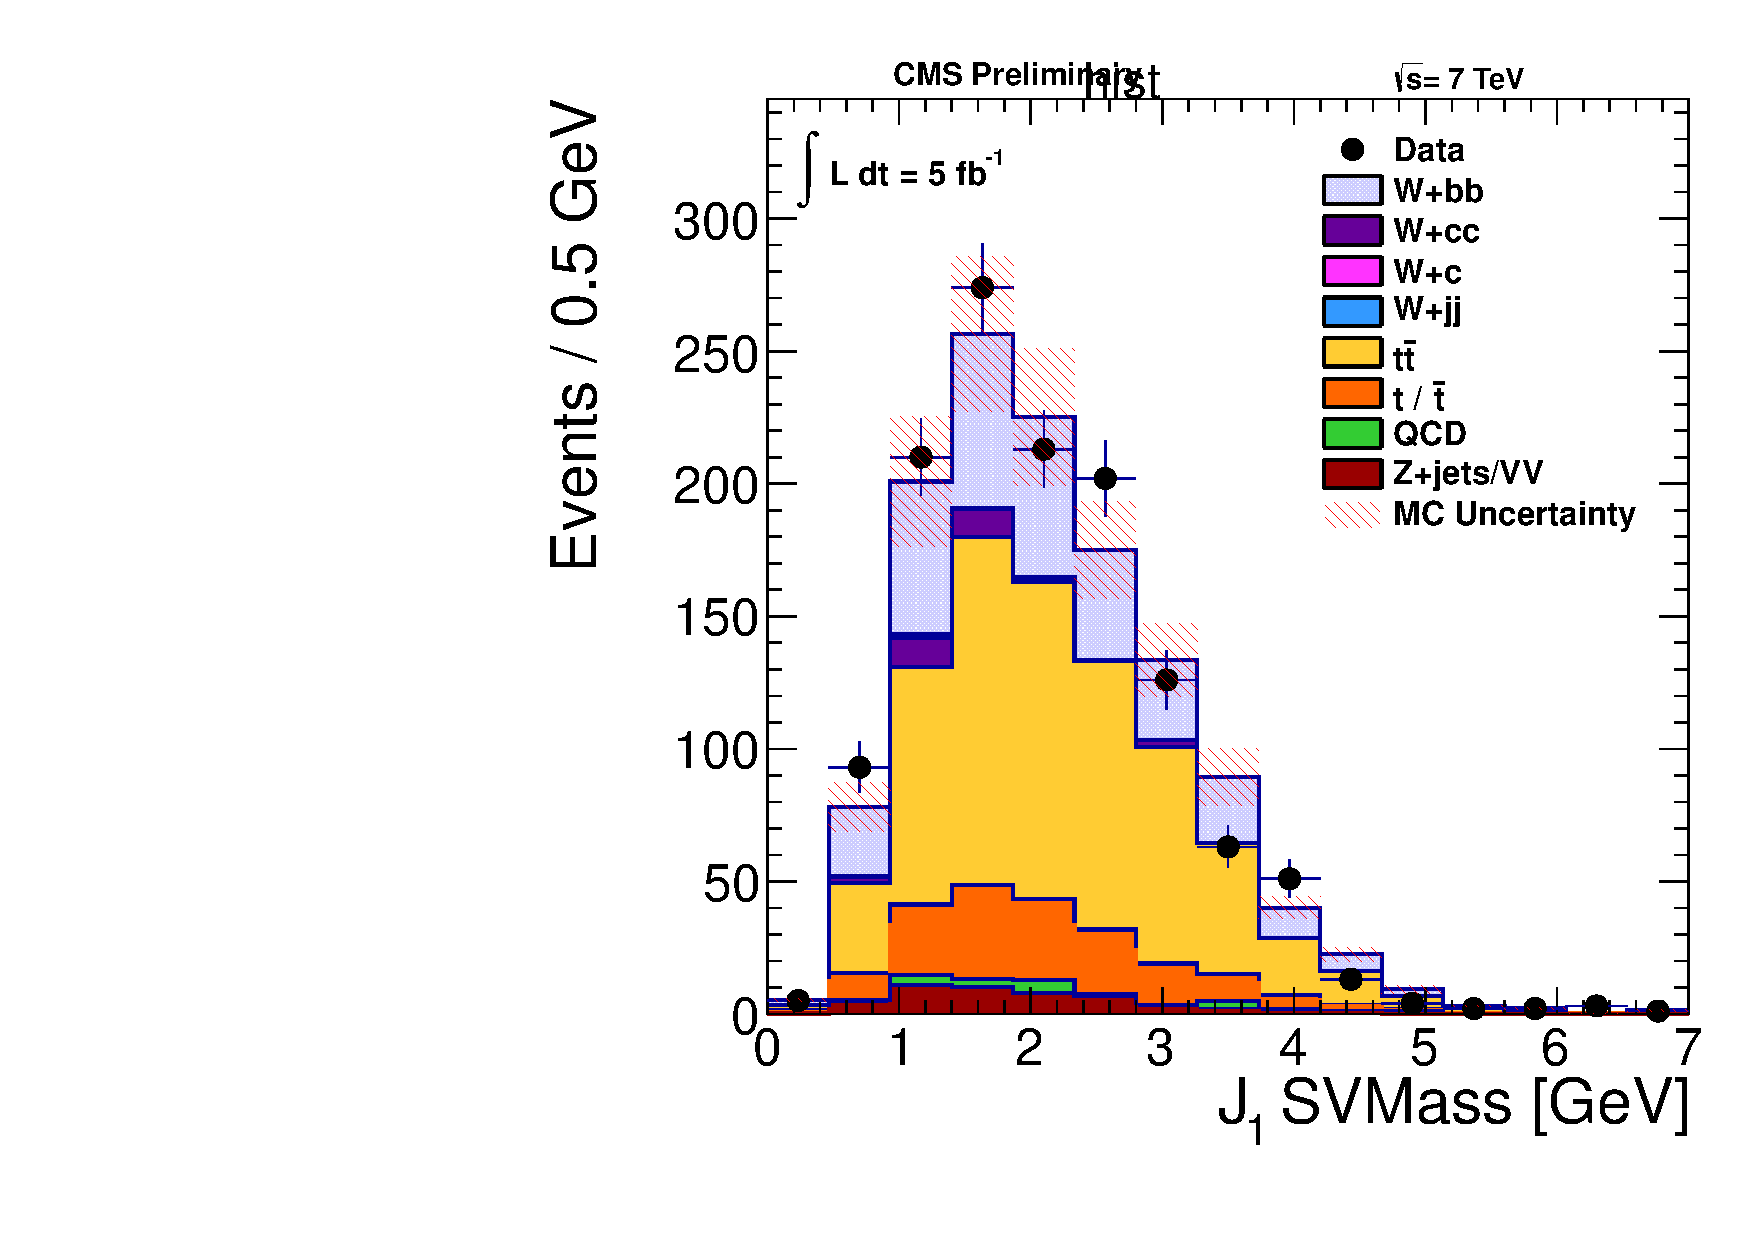
\includegraphics[width=0.47\textwidth]{Wbb/fig1a_J1Mass.pdf}
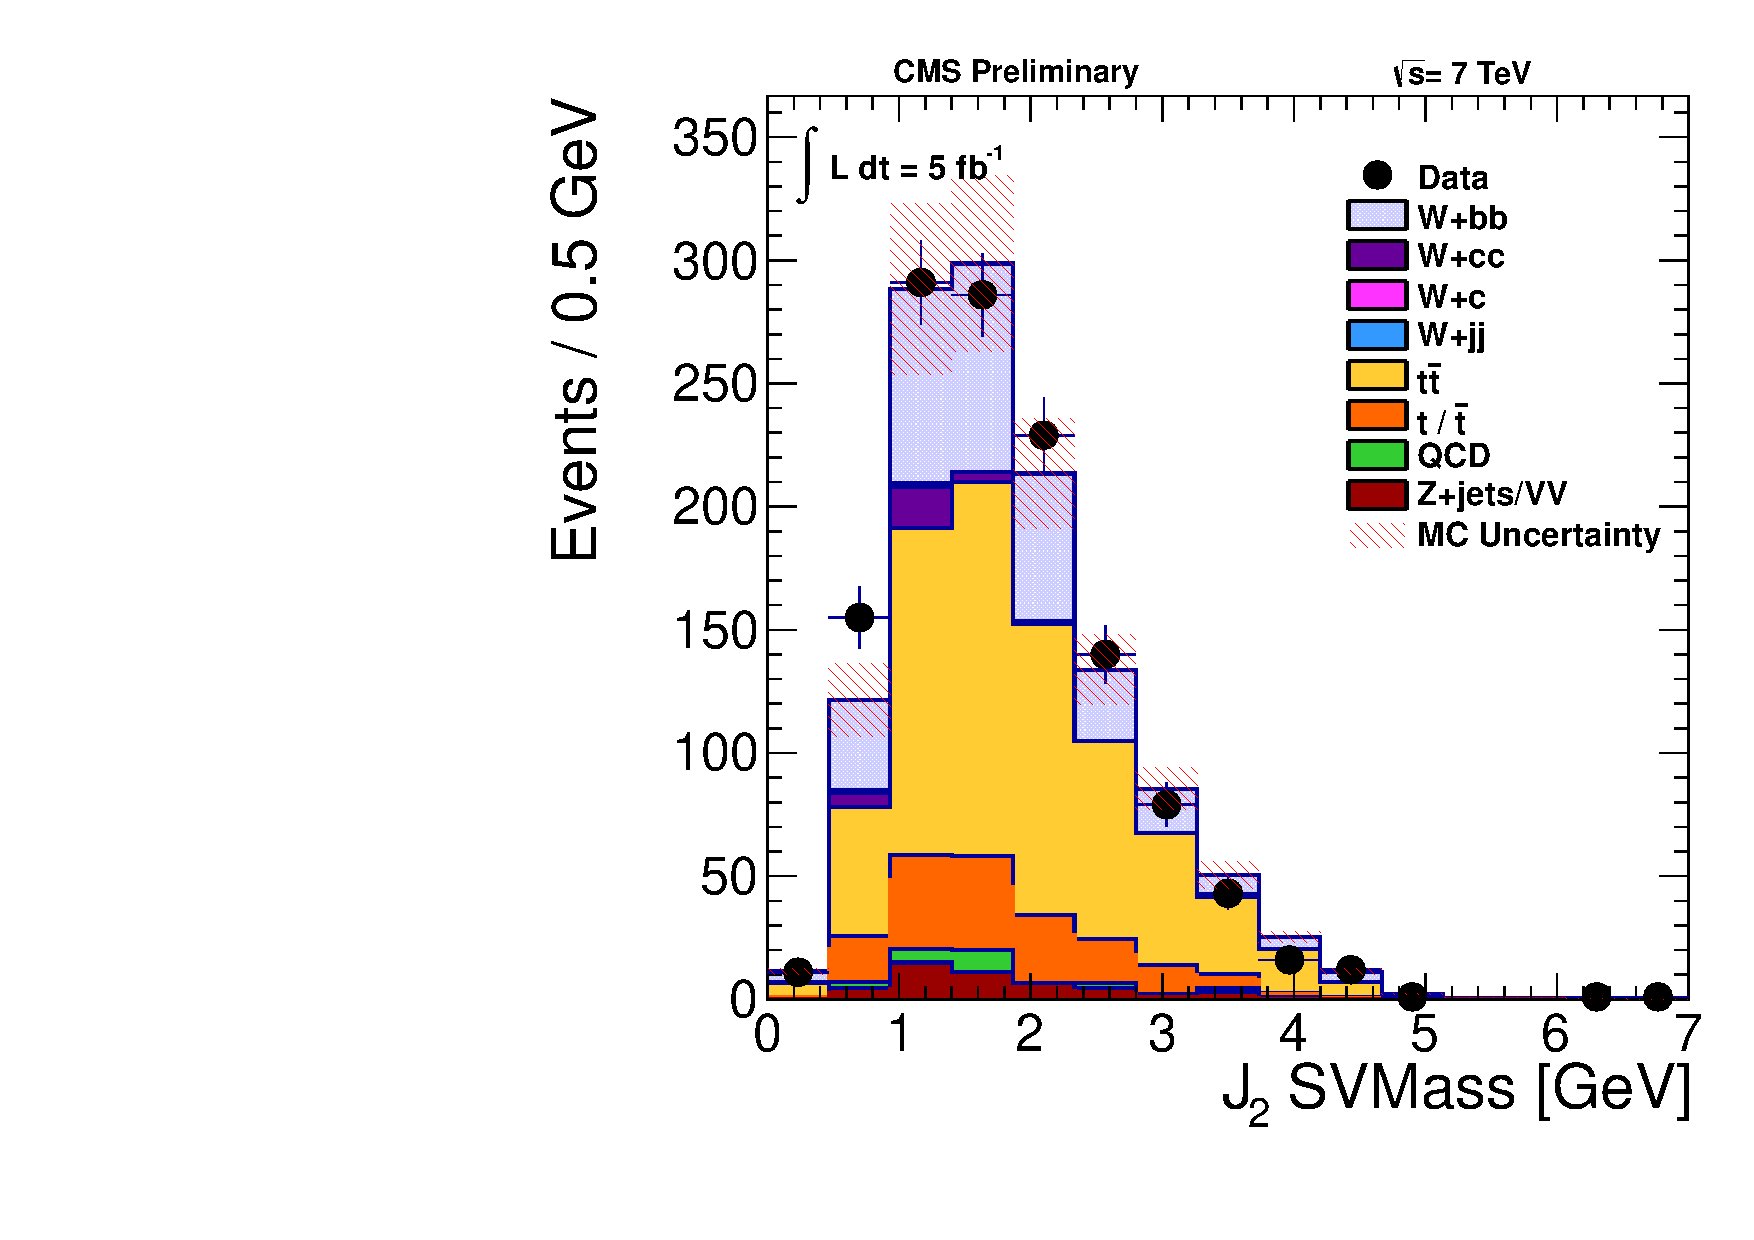
\includegraphics[width=0.47\textwidth]{Wbb/fig1a_J2Mass.pdf}
\caption{Mass of the secondary vertex for the highest-$p_{T}$ jet ($\rm{J_{1}}$, right) and for the second jet ($\rm{J_{2}}$, left) in the signal region.}
\label{fig:figAbis}
\end{figure}

\subsection{Top backgrounds}
The events selected for the $\ttbar$ control region pass the selection requirements, with
no restrictions on the number of leptons in the event. 
In addition to the two highest-$\pt$ b-tag jets, the events are required to have at least two extra light jets.
This higher jet multiplicity requirement selects a sample that is dominated by $\ttbar$ events.
Figure~\ref{fig:figB} (right) shows the invariant mass of the 
two highest-$\pt$ additional jets (3rd and 4th highest-$\pt$ in the event, $m_{\rm{J_{3}J_{4}}}$). 
In $\ttbar$ events this distribution reconstructs the mass of the hadronically decaying W boson. 
It is used in the final fit to extract the $\ttbar$ background normalization.
% CHECK: Add info on JES? JER?
The simulation describes the observed distributions well both in 
shape and normalization.

%\begin{figure}
%\centering
%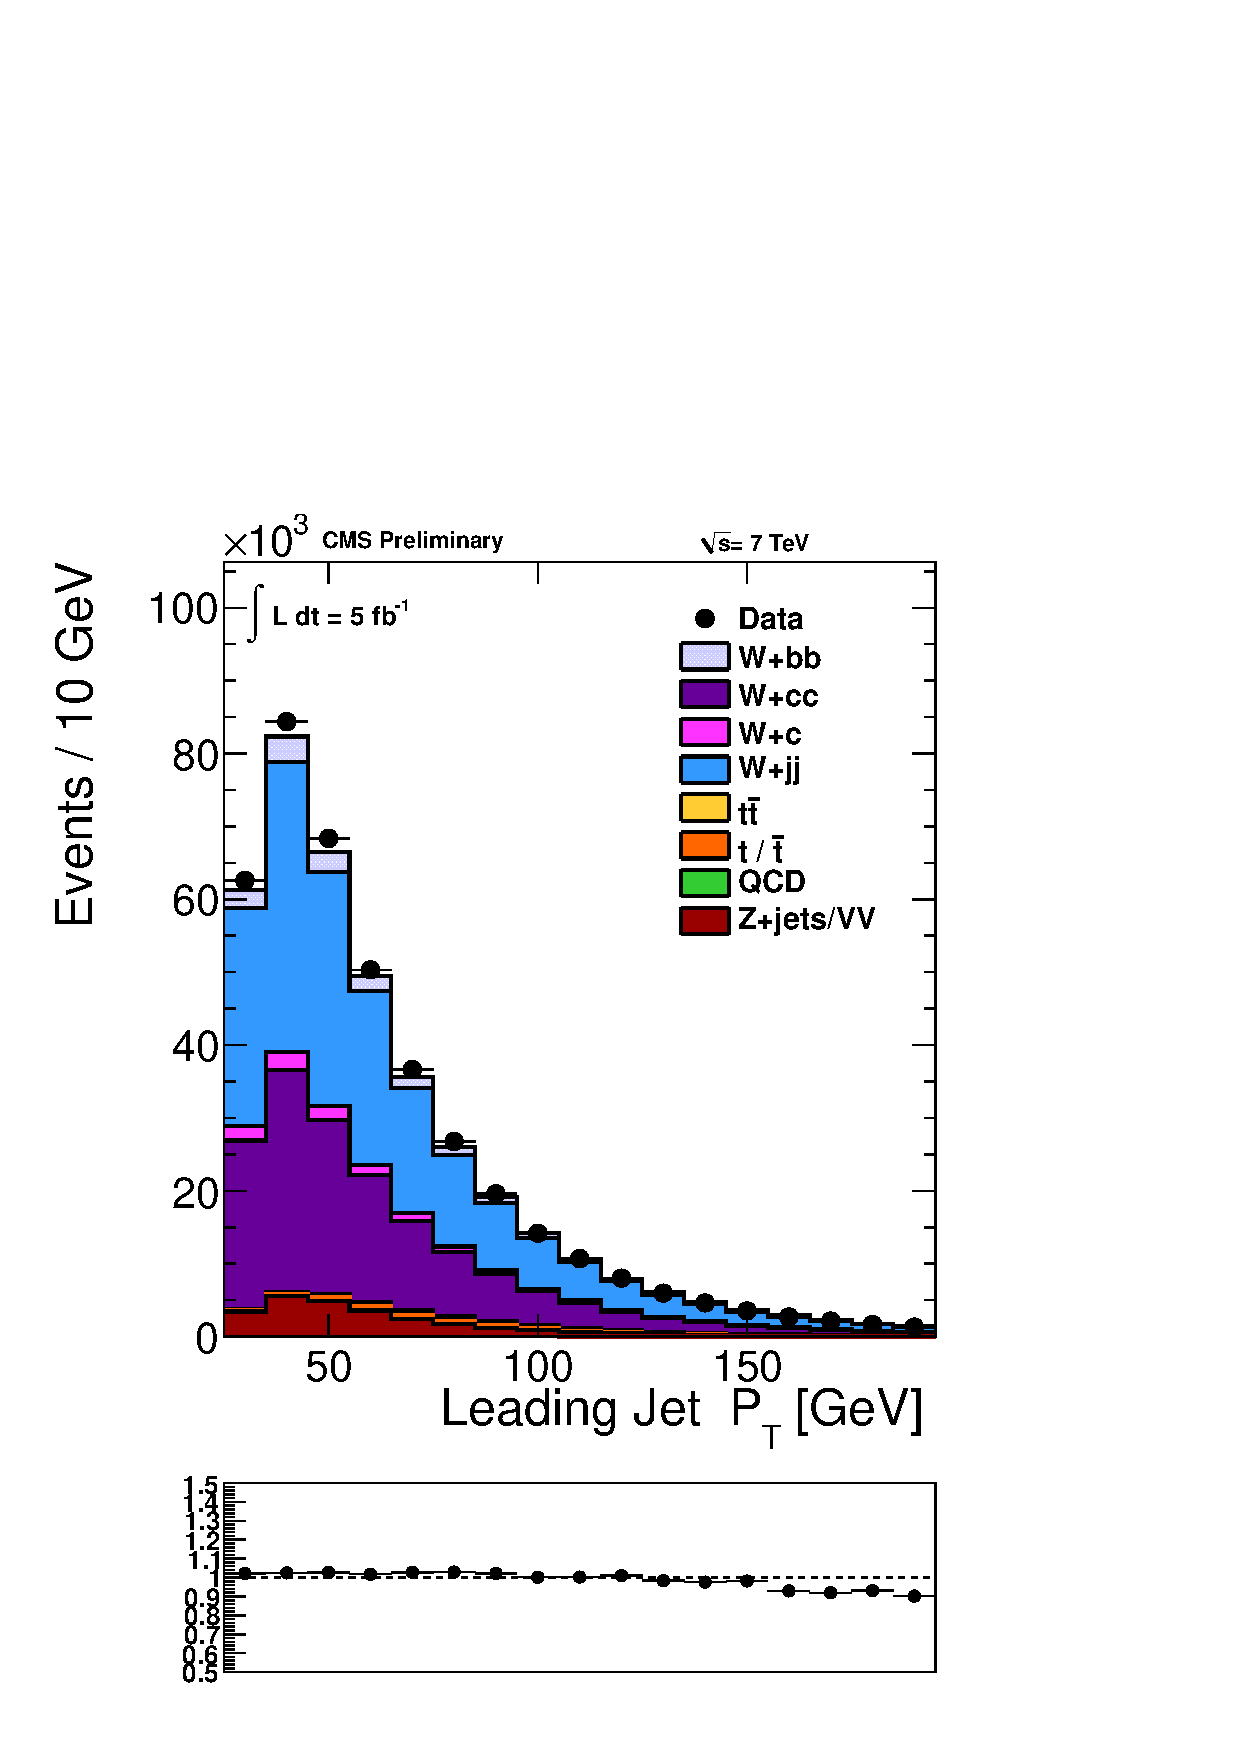
\includegraphics[width=0.45\textwidth,trim = 0 4cm 0 0, clip=true ]{Wbb/fig1.pdf}
%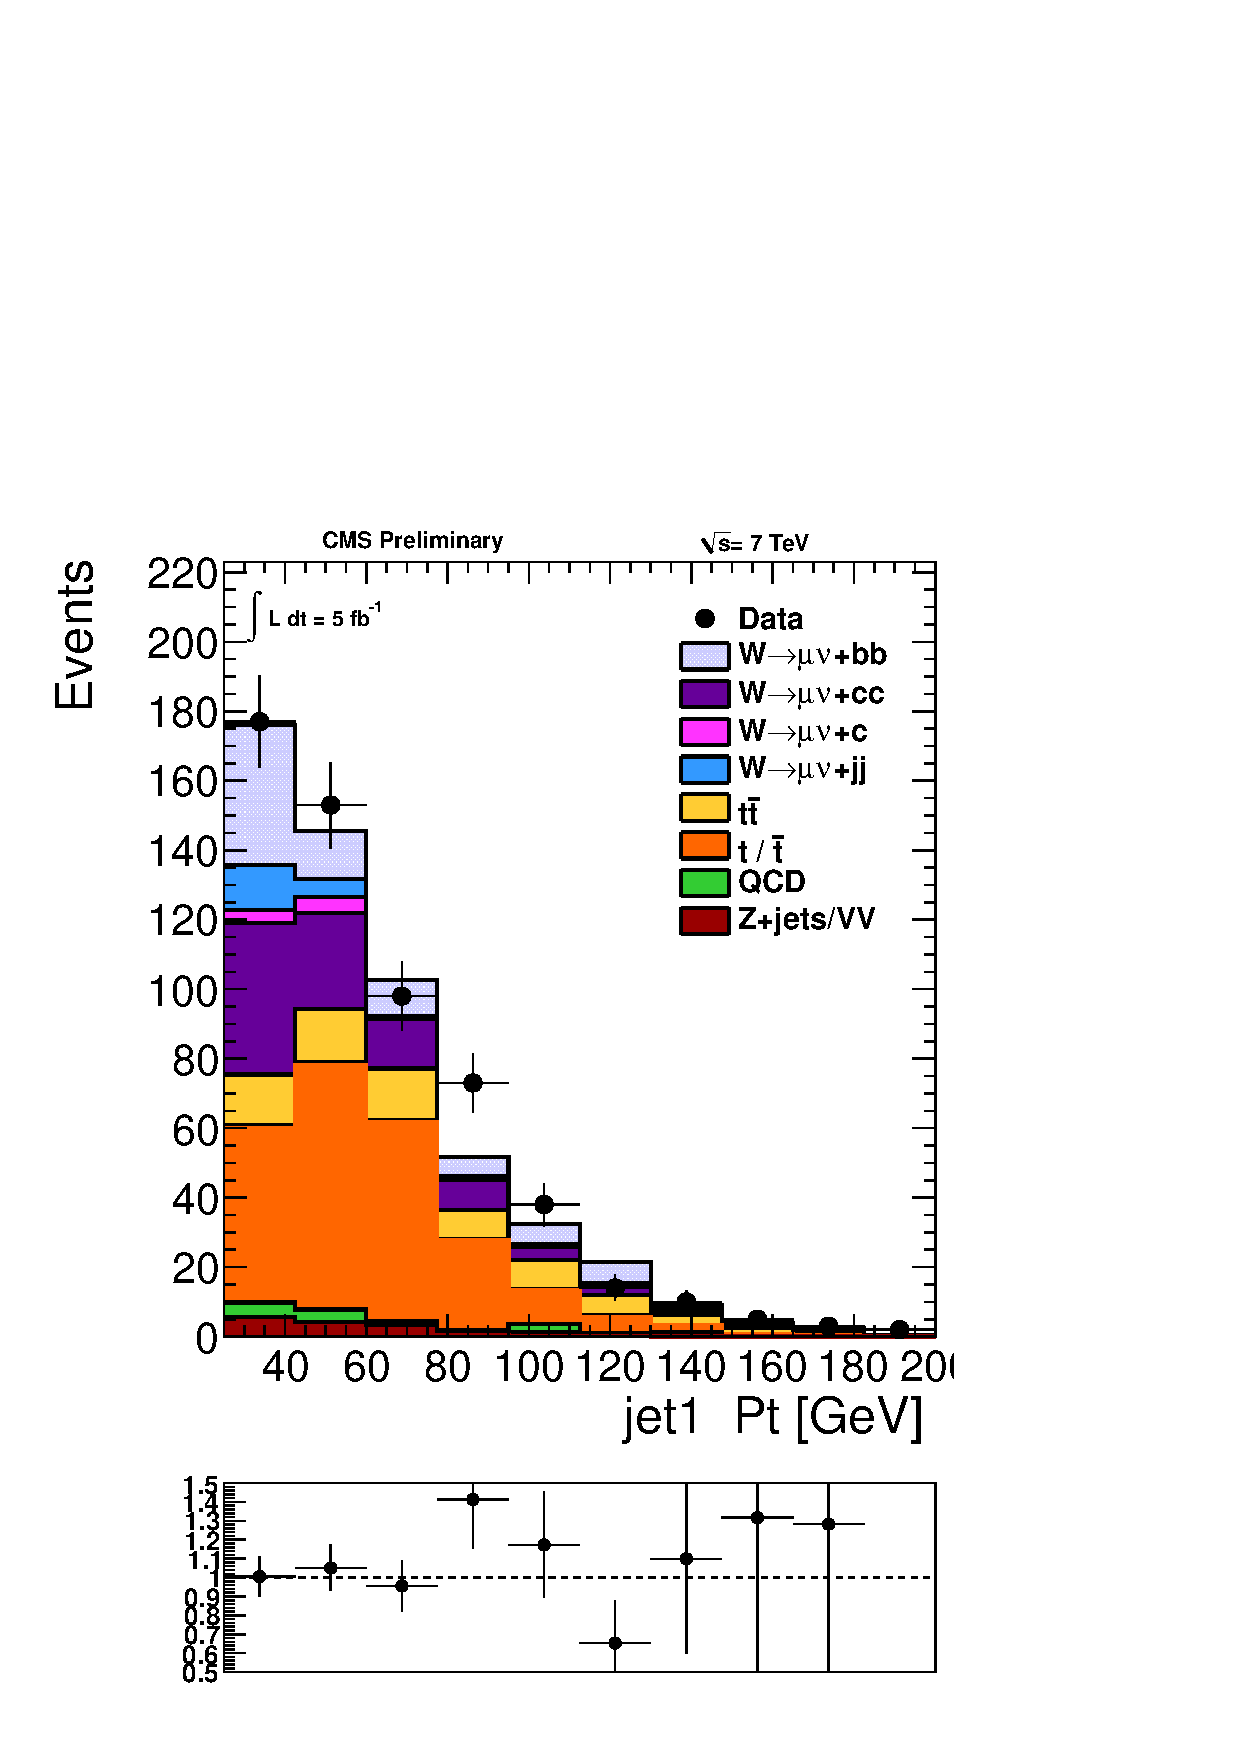
\includegraphics[width=0.45\textwidth,trim = 0 4cm 0 0, clip=true ]{Wbb/fig2.pdf}
%\caption{(left) The $\pt$ of the leading-\pt jet, before applying SV and CSV requirements 
%(right) b-tag jet \pt in the single top control region}
%\label{fig1}
%\end{figure}

A single-top-quark control region is defined by selecting events in which the
W boson is accompanied by exactly one b jet
passing the described tagging criteria, and an additional forward jet with $|\eta|>$2.8.
No additional vetoes on extra light jets or leptons are applied.
%The events selected for the single-top control region pass the selection requirements 
%except that events with
%extra jets and leptons are allowed. In addition, events with only one b-tagged jet are 
%selected and at least one
%jet is required to have $|\eta|>$2.8.
%Figure~\ref{fig1}(right) shows the $\pt$ of the b-tag jet in this
%control region. 
As seen in figure \ref{fig:sTopMT}, the simulation describes the single-top production control region
well and therefore
it is used to estimate the yield and shape of the single top contribution in the signal region.

\begin{figure}
      \center
          \begin{subfigure}[b]{.47\textwidth}
      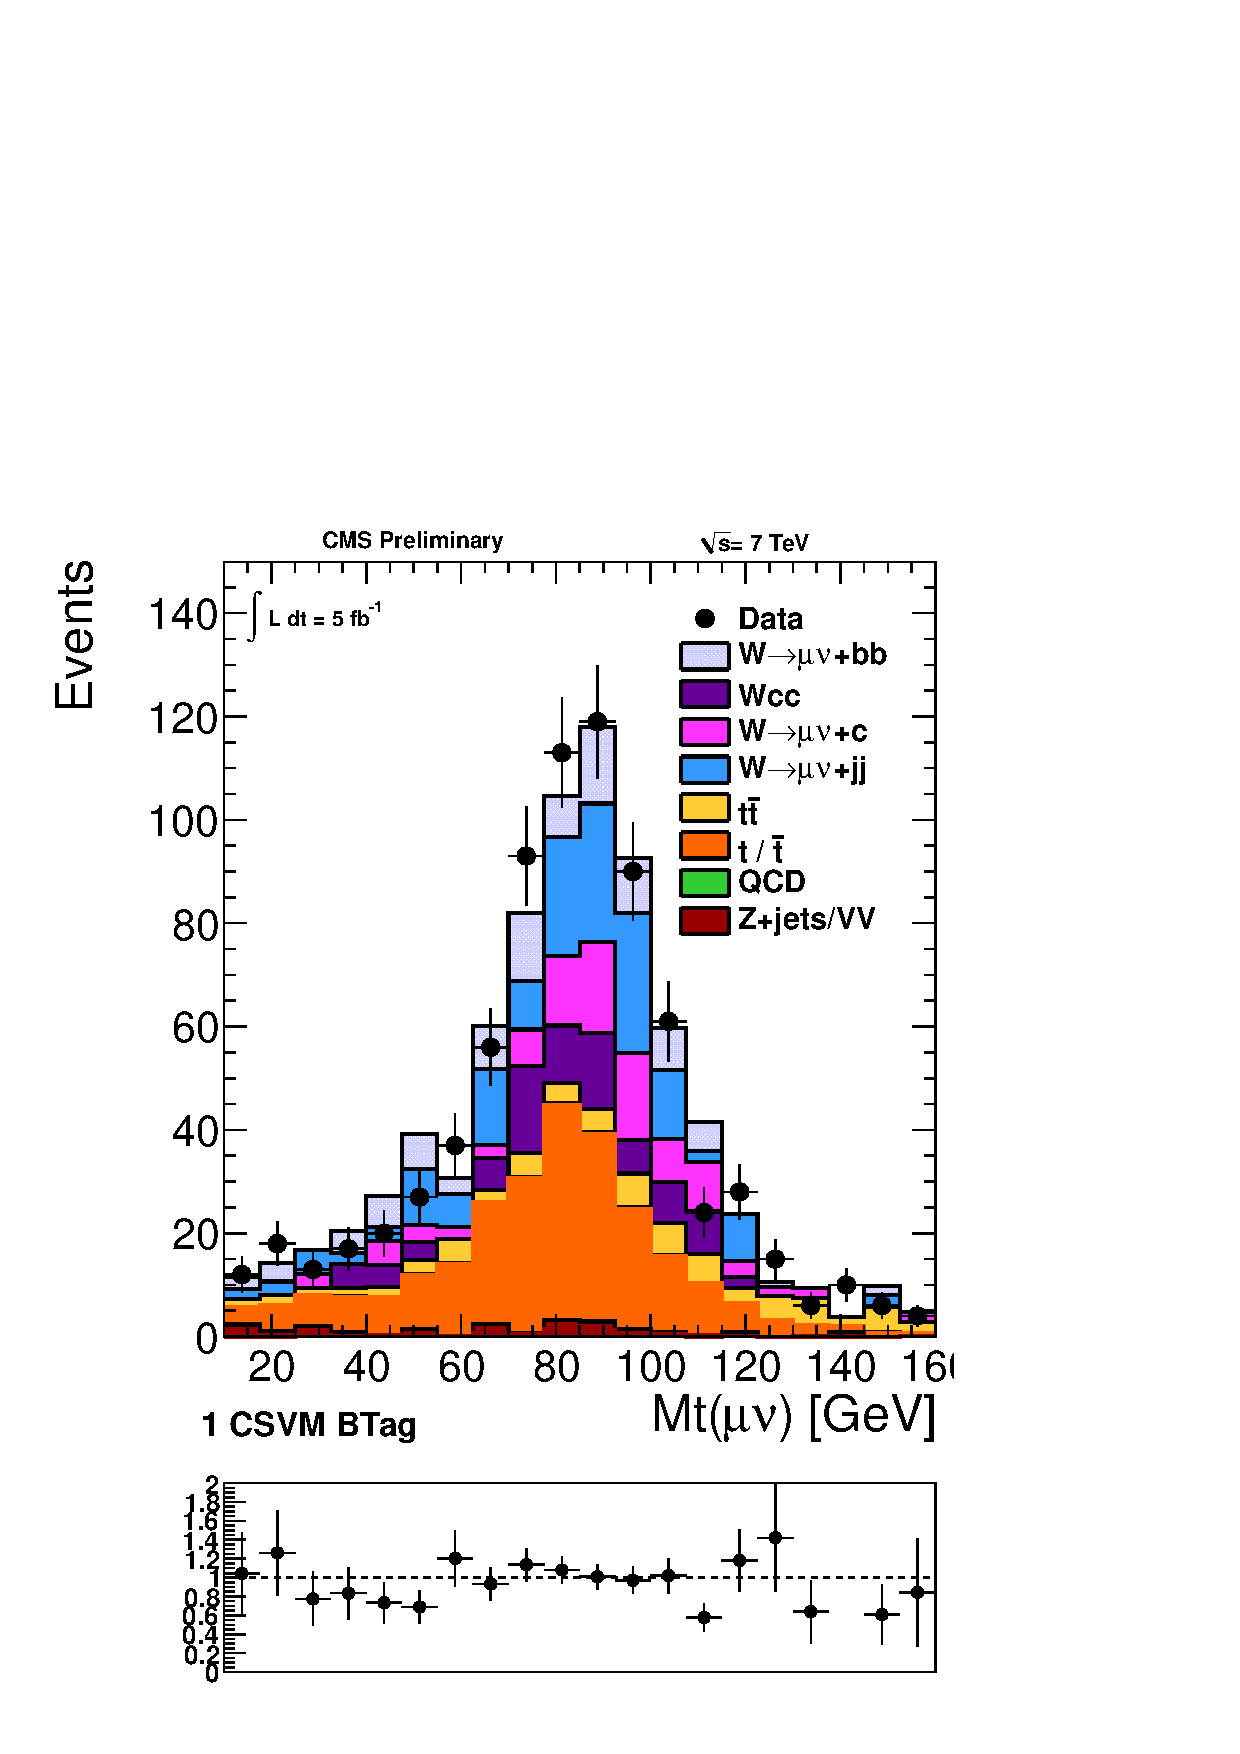
\includegraphics[width=\textwidth, trim = 0 5.2cm 0 0, clip=true ]{Wbb/MtCal_SingleTop.pdf}
    \caption[]{$M_{T}$    [GeV]}
    \end{subfigure}
    \begin{subfigure}[b]{.47\textwidth}
      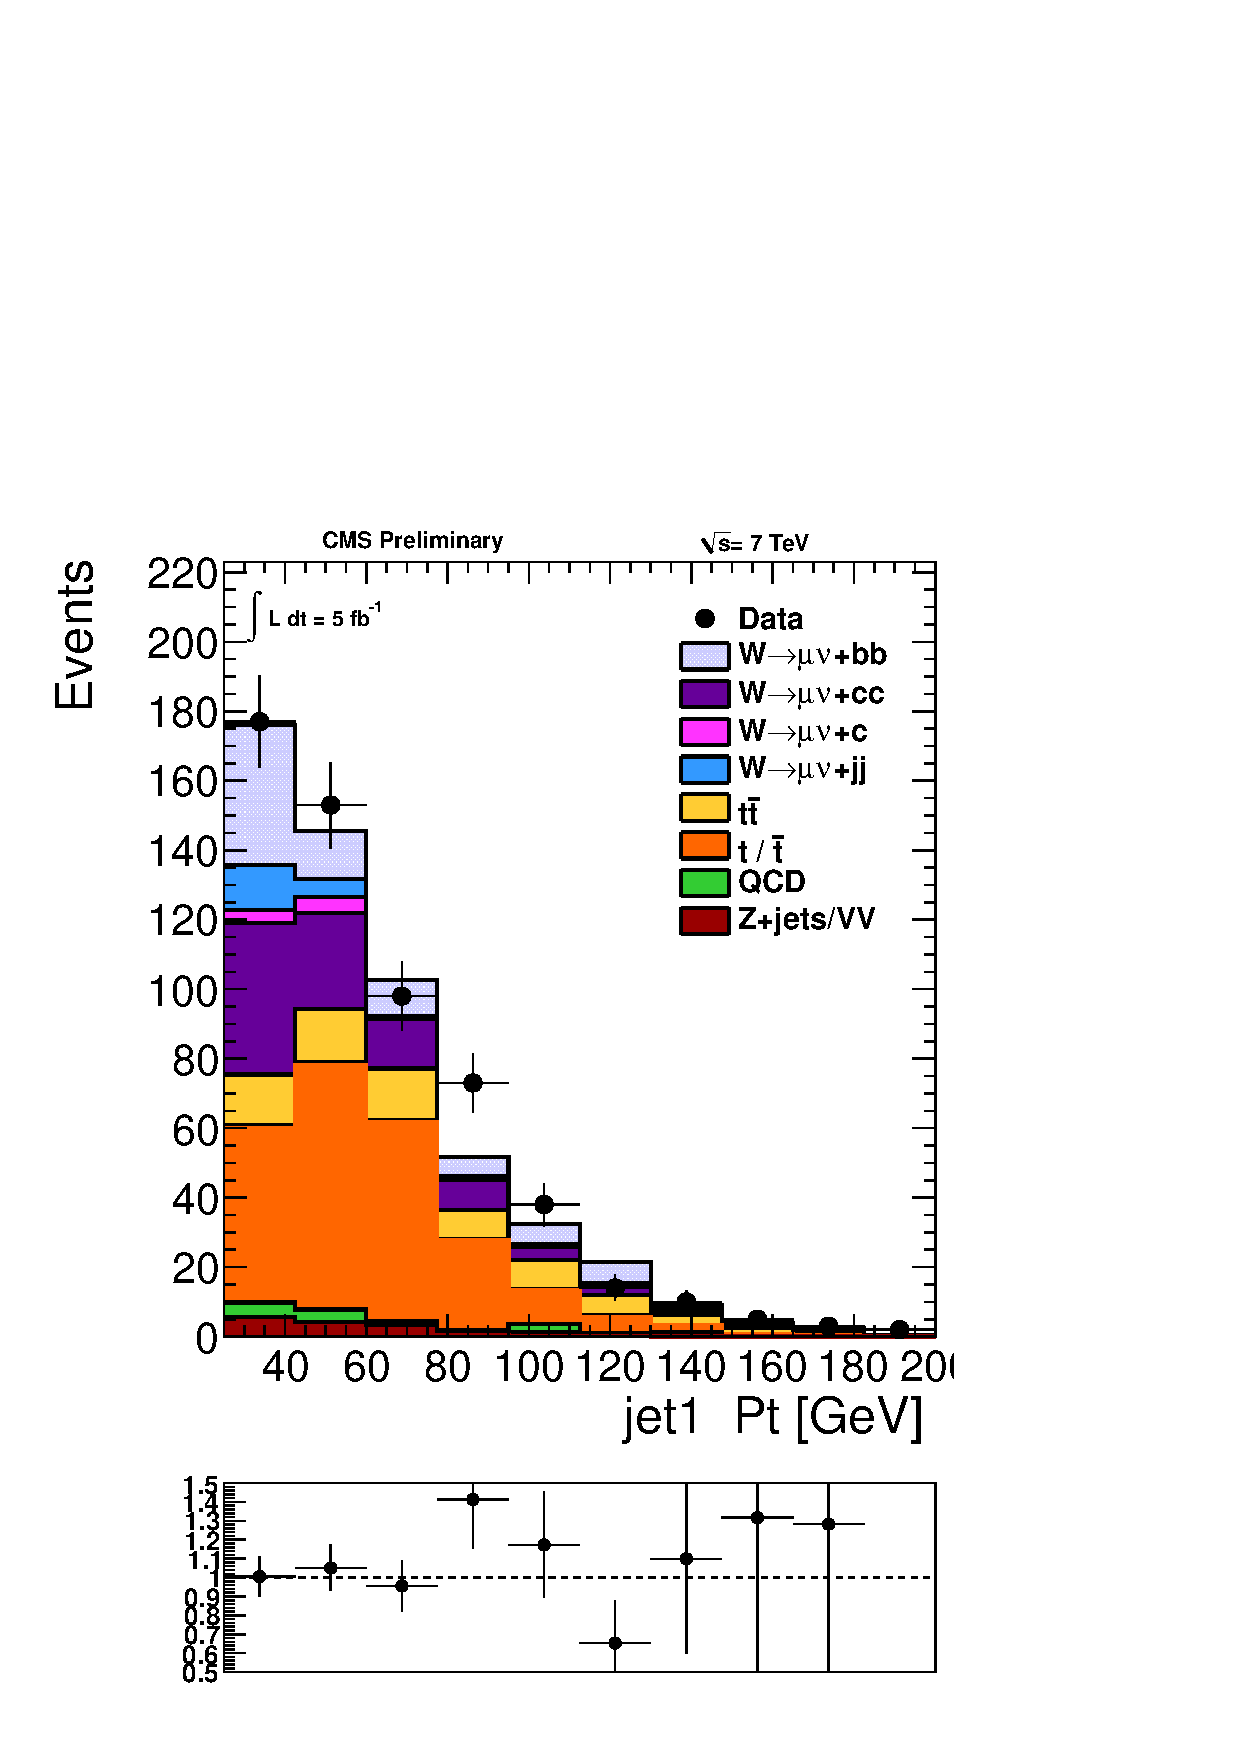
\includegraphics[width=\textwidth, trim = 0 5.2cm 0 0, clip=true ]{Wbb/highestJetPt_J1Pt_top.pdf}
    \caption[]{Leading Jet $p_{T}$    [GeV]}
    \end{subfigure}
      \caption{The single top control region defined by one (b)-tagged jet 
      and one forward jet at ($\eta\>$2.8). Both the transverse mass of 
      the selected W in the $t\rightarrow b \mu \nu$ process (left) and 
      the pt of the leading jet (right) show agreement with the
Monte Carlo prediction.}
      \label{fig:sTopMT}
\end{figure}


\subsection{Z Background}
The Z+jets background estimate is validated in a control region where the standard selection 
is applied except that a second muon is required,  $ 70 < m_{\mu\mu} < 100GeV$. 
As seen in figure \ref{fig:Z_DiMuonMass_met}, agreement
between the observed distributions and simulation is observed in this region.

\begin{figure}[b]
    \center
    \begin{subfigure}[b]{.47\textwidth}
    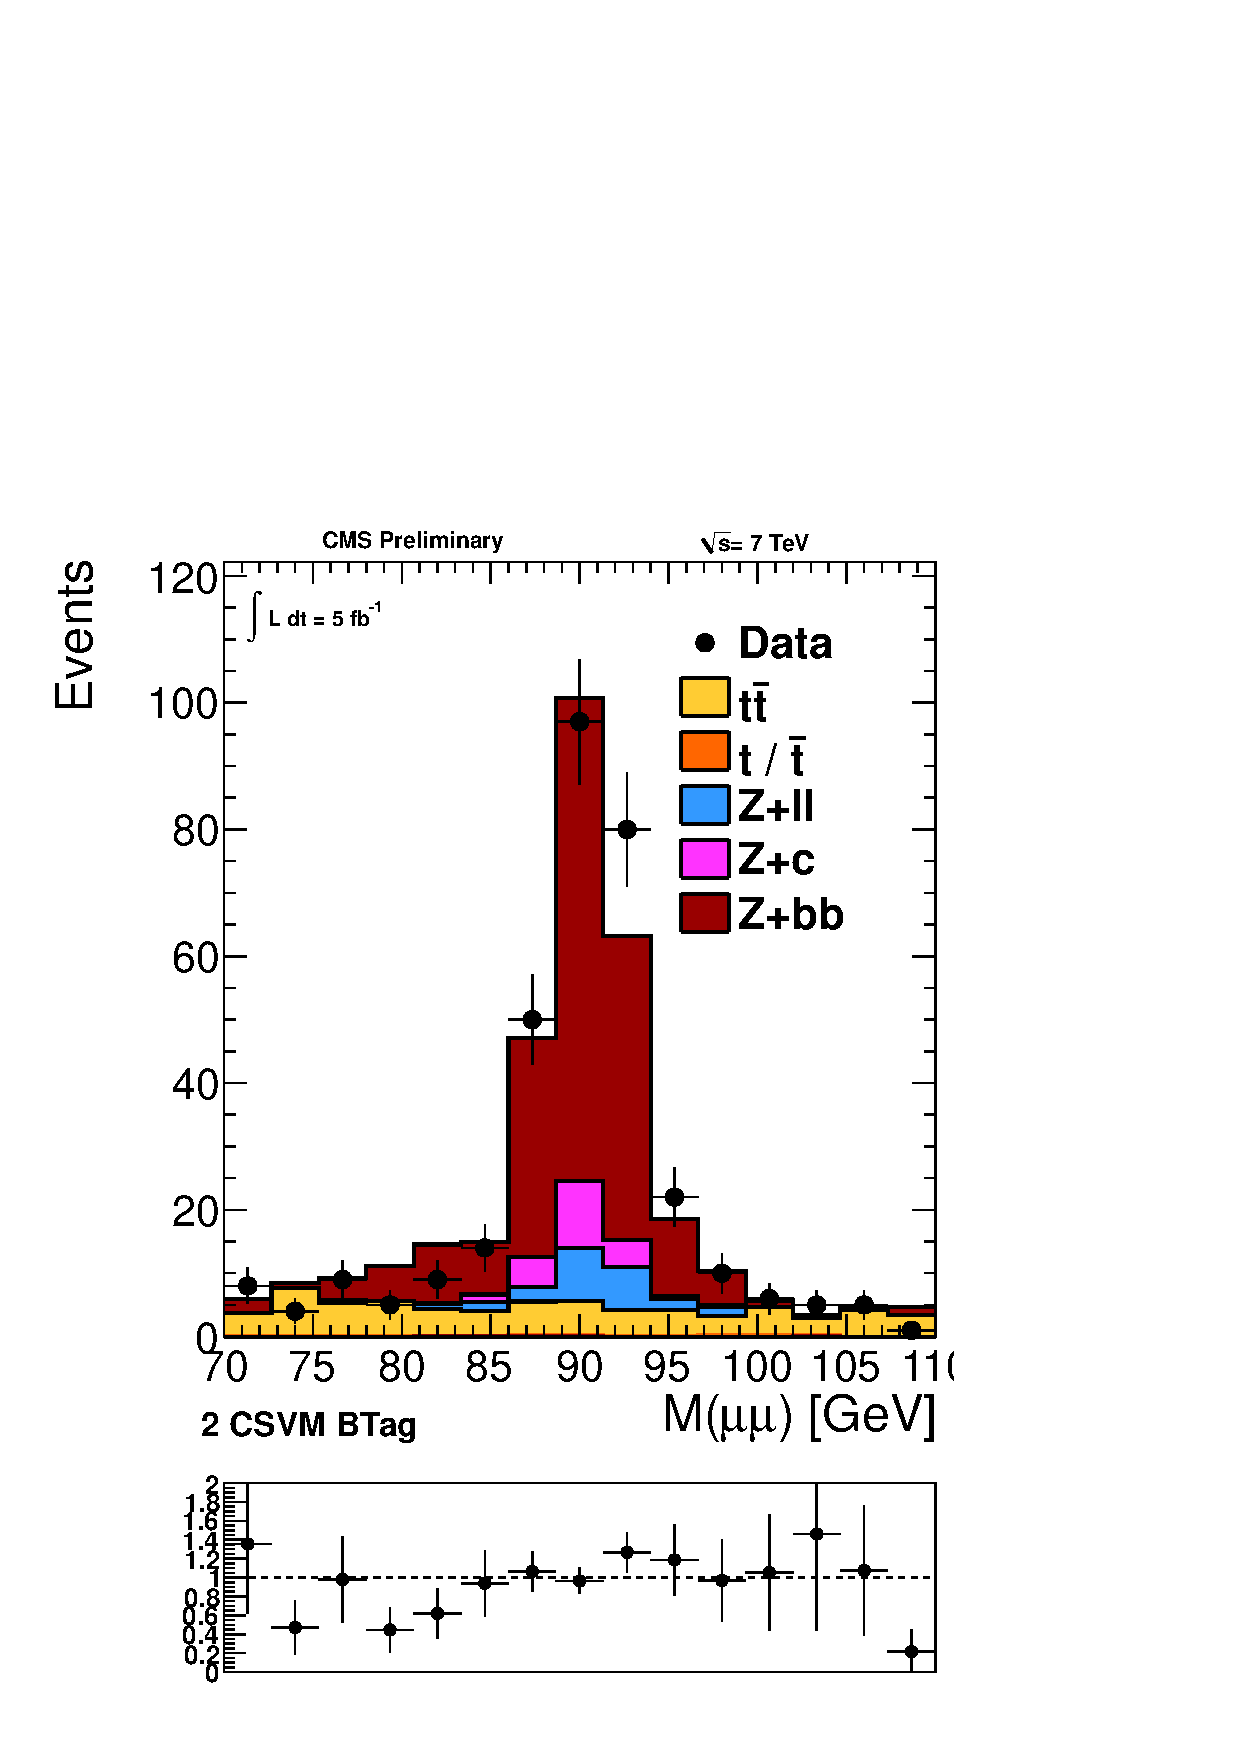
\includegraphics[height=6.5cm, trim = 0mm 52mm 0mm 0mm, clip,width=\textwidth]{Wbb/DiMuonMass.pdf}
    \caption[]{$M_{ll}$    [GeV]}
\label{fig:DiMuonMass}
    \end{subfigure}
\begin{subfigure}[b]{.47\textwidth}
    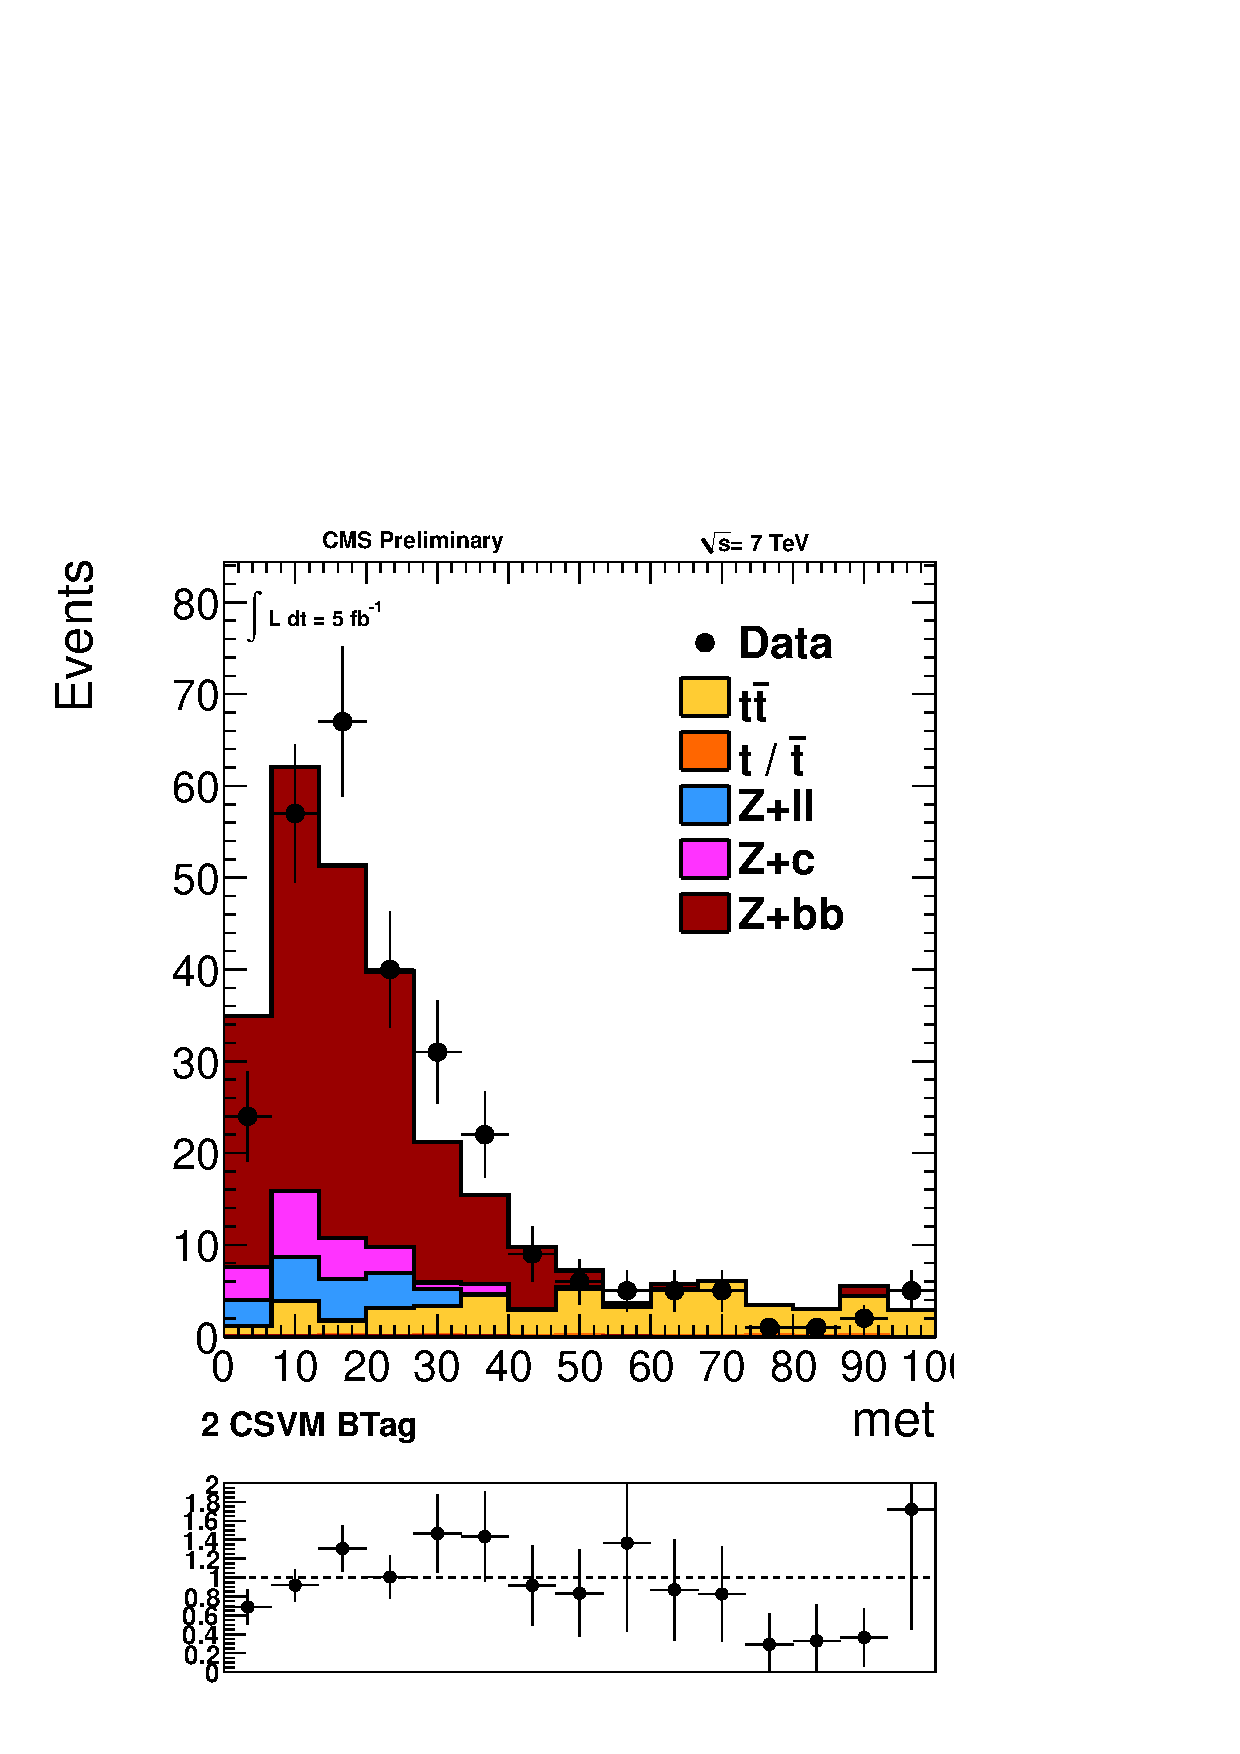
\includegraphics[height=6.5cm, trim = 0mm 52mm 0mm 0mm, clip,width=\textwidth]{Wbb/Z_met.pdf}
    \caption[]{$E_{T}^{miss}$    [GeV]}
    \label{fig:Z_met}
        \end{subfigure}
    \caption{In the Z+jets control region the invariant mass of the Z (left), and 
      the $E_{T}^{miss}$ (right)}
    %\caption{Leading Order Decay Mode for \Wmnbb}                                                                                         
    \label{fig:Z_DiMuonMass_met}
  %\end{center}                                                                                                                            
\end{figure}


\begin{figure}[t]
\centering
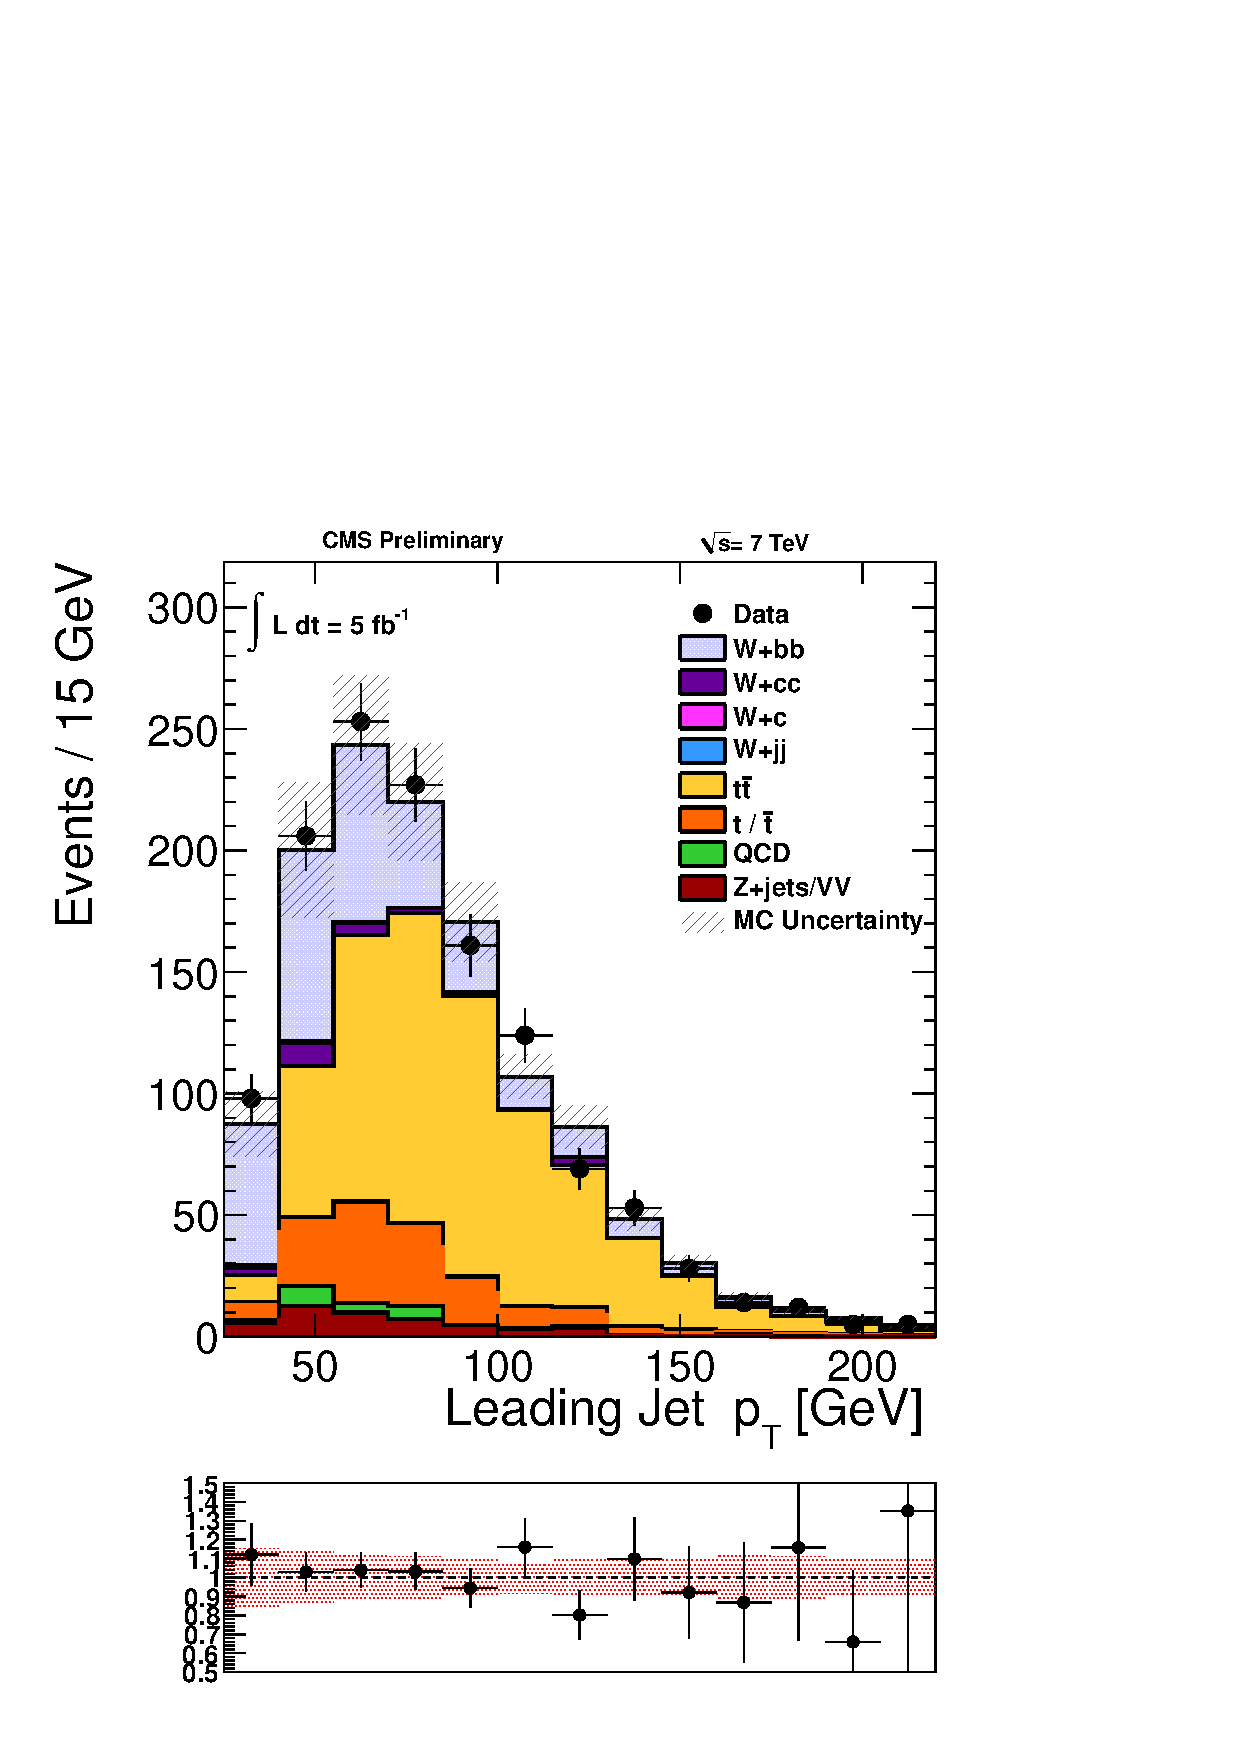
\includegraphics[width=0.45\textwidth, trim = 0 4cm 0 0, clip=true ]{Wbb/fig4.pdf}
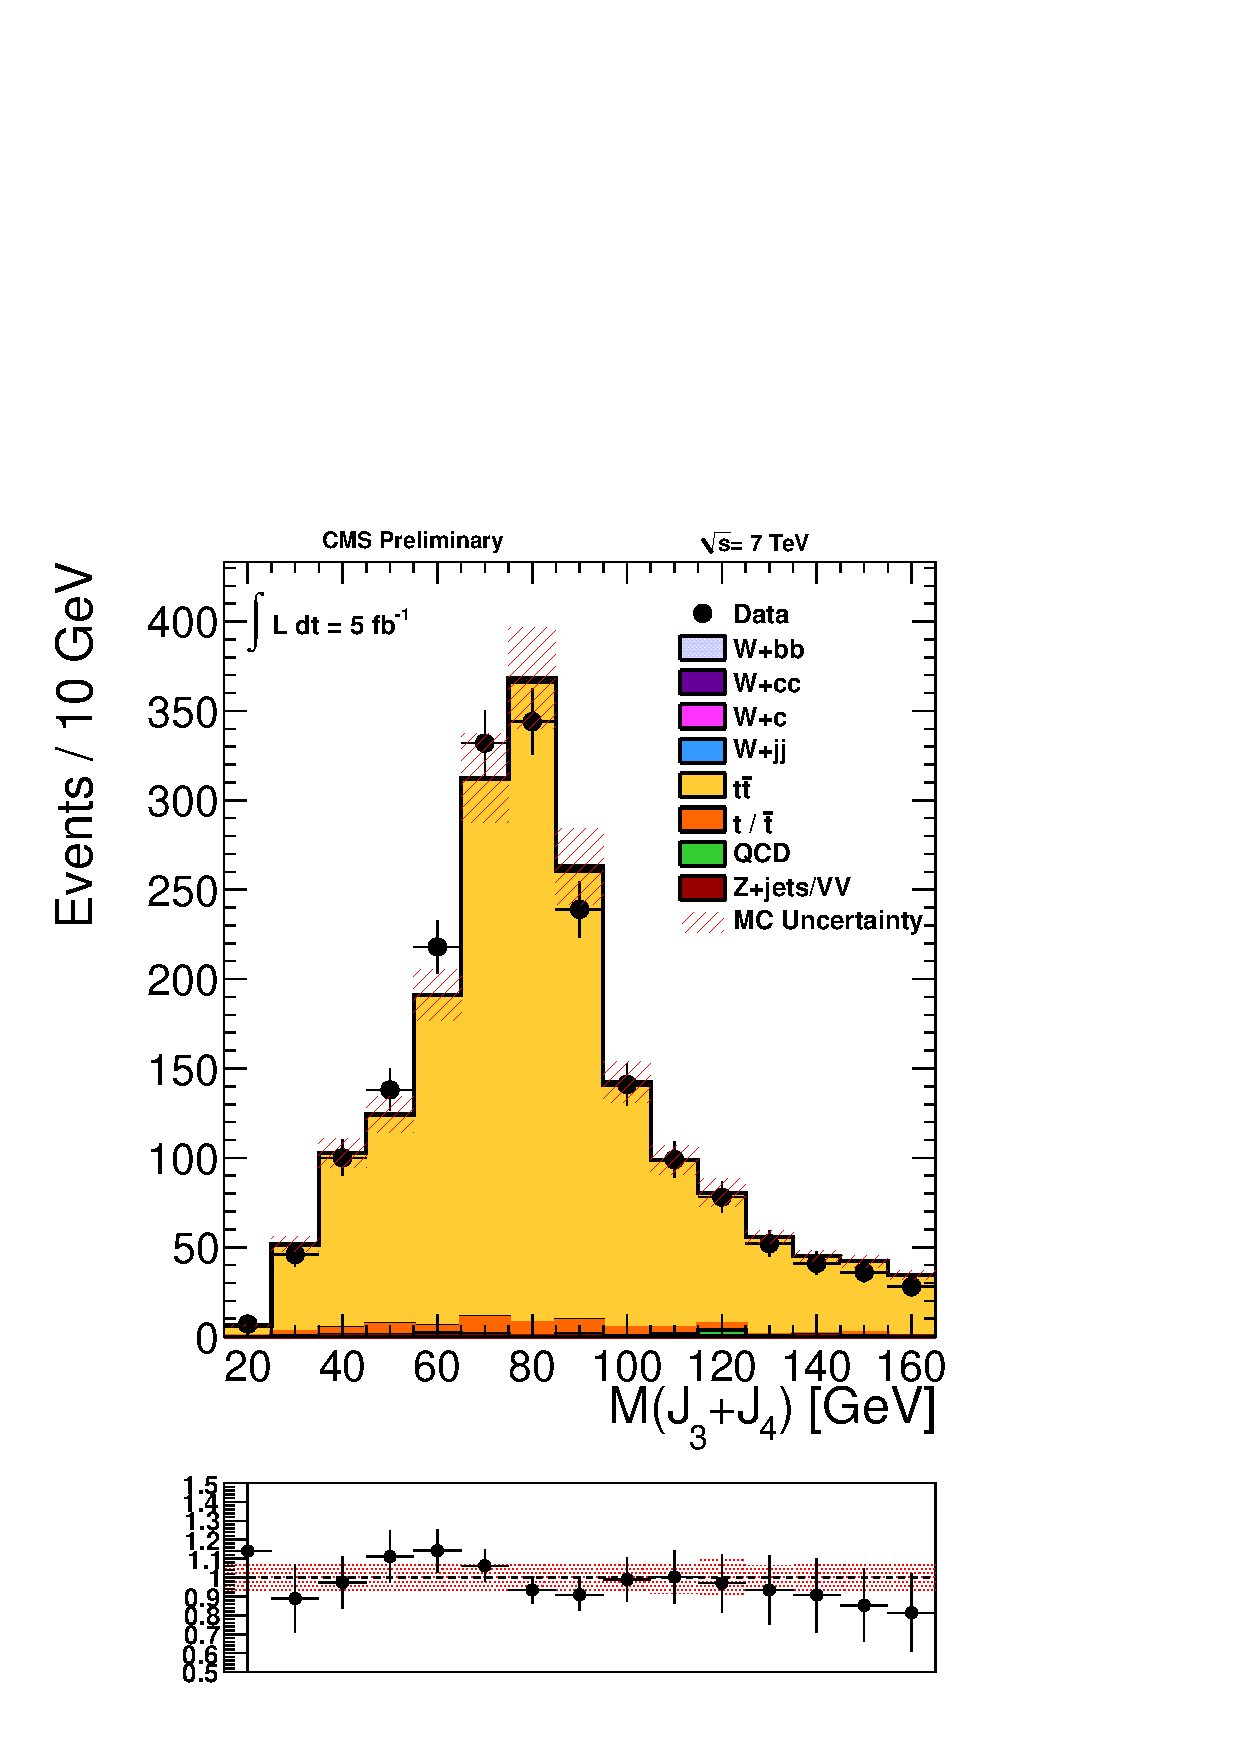
\includegraphics[width=0.45\textwidth, trim = 0 4cm 0 0, clip=true ]{Wbb/fig3.pdf}
\caption{ 
(left) The $\pt$ distribution of the highest-$\pt$ jet in the signal region, normalized to the result of the binned maximum likelihood fit.
(right) The invariant mass of the two additional light jets in the $\ttbar$ control region, also
normalized to the results of the fit.
}
\label{fig:figB}
\end{figure}

\subsection{Systematic Uncertainties}
One of the dominant systematic uncertainties comes from the 
relative uncertainty on the b-tagging efficiency ($6\%$ per jet) is taken from Ref.~\cite{BTAGNOTE}
along with the uncertainty of the light and charm 
jet mistagging efficiencies are.
The jet and muon energy scales are allowed to vary up and down by one standard deviation and
are added to the fit as a binned shape variation.
The uncertainty associated to the pileup description in 
Monte Carlo is estimated by shifting the overall mean of 
the number of vertices up or down by 0.6 bunch crossings; it has a negligible effect on the analysis.
To account for the $\MET$ uncertainty the component of $\MET$ that 
is not clustered in jets is scaled by $\pm10\%$.
Uncertainties on the muon efficiency estimation 
(triggering, identification, isolation) are estimated to be 1\%.
Background normalization is also taken into account, with an uncertainty assigned to each process
according to previous CMS measurements or to the described control regions. 
The luminosity uncertainty, 2.2\%, 
is taken from Ref.~\cite{CMS-PAS-SMP-12-008}.


\subsection{Final Yield Extraction}
\label{sec:finalfit}
The final yields are extracted via a binned maximum likelihood fit.
To constrain the most prominent backgrounds and reduce the final
systematic uncertainty the fit is performed simultaneously on the $\pt$ of the leading jet ($\rm{J_1}$) 
in the signal region after all selection requirements have been applied,
and on the $m_{\rm{J_3 J_4}}$ distribution obtained from the $\ttbar$ control region.
The  $\rm{J_1}$ $\pt$  is chosen as the final fit variable due to its discrimination power against top-related backgrounds.
Figure~\ref{fig:figB} shows the two fitted distributions, $\pt^{\rm{J_1}}$  in the signal region (left)
and $m_{\rm{J_3 J_4}}$ in the $\ttbar$ control region (right), normalized to the results of the fit.

The statistical and systematic uncertainties are introduced in the form of
nuisance parameters via log-normal distributions around the estimated central values.
The fitted yields for each one of the processes can be found in Table~\ref{tab:fitYields}, 
compared to the Monte Carlo predictions.
To calculate the final uncertainties, first the          
total errors are calculated by taking both
the statistical and systematic errors into
account in the fit. Then the systematic nuisance parameters are removed, the fit is re-run
and the statistical uncertainty is 
obtained. The total systematic error is calculated by subtracting in quadrature 
the statistical uncertainty from the total error.


\begin{table}[b]
\begin{center}
\begin{tabular}{c c c }
\hline 
Process  & Prediction  & Fitted Yield \\
\hline 
$\Wbb$         & $332\pm66$     & $300\pm60$ \\
$\Wc$, $\Wcc$  & $21\pm4$       & $20\pm4$ \\
W+usdg         & $1.5\pm0.2$    & $1\pm1$  \\
Z+jets         & $31\pm3$       & $32\pm3$ \\   
$\ttbar$       & $596\pm35$     & $647\pm52$ \\  
Single top     & $160\pm13$     & $170\pm13$ \\
WW, WZ         & $19\pm3$       & $17\pm3$   \\
QCD            & $33\pm17$      & $33\pm16$  \\
\hline
Total          & $1194\pm78$    & $1220\pm82$ \\ 
\hline 
\hline
Observed Events & \multicolumn{2}{c}{$1230\pm35 $} \\
\hline 
\end{tabular}
\caption{Comparison of the expected (before the fit) and measured (after the fit) yields for each of the processes. The uncertainty on
the Monte Carlo prediction takes into account the variation allowed to the nuisance parameters in the fit. The uncertainty in the fitted yields
corresponds to the full uncertainty after the fit.
}
\label{tab:fitYields}
\end{center}
\end{table}

The observed number of events in data after selection in the signal region is $N(S+B)_{data}=1230\pm35 $. 
The number of signal events obtained in the binned maximum likelihood fit is $300\pm60$. 

\subsection{Alternate Approach}
To show the robustness of the $\Wbb$ fit result a separate study was performed with
two selected b-tagged jets that require each jet to fulfill a looser CSV b-tagging criterion, corresponding 
to an efficiency  of 70\%
for jets containing b-flavored hadrons, while the misidentification probability for light-quark jets is 1$\%$.
%%%% Note that TOP-12-024 quotes 60% - 1% 
With the exception of the modification to the CSV threshold, all other selections for the signal
and control region remain unchanged. The $\Wcc$ contribution is non-negligible with this selection,
therefore, the sum of the invariant mass of the secondary vertex found in each selected jet
is used to distinguish between $\Wbb$ and $\Wcc$. The scalar sum of the transverse momenta of the
muon, the $\vecEtm$ and the jets,
$H_{\rm{T}}$, is used to distinguish W+jets from
top contributions. 
The $\Wbb$ signal is extracted via a two dimensional fit of 
$H_{\rm{T}}$ versus
the sum of the the  secondary vertex masses of the highest- ($\rm{J_1}$) and second-highest-$\pt$ ($\rm{J_2}$) jets. 
An equivalent $\ttbar$ control region to the one described in the
tighter selection, based on the reconstruction of the W mass using two light jets, is also used in this case.
The variables $\rm{J_1}$ SV mass + $\rm{J_2}$ SV mass and $H_{\rm{T}}$ are shown in Fig.~\ref{fig:figC}, with yields 
normalized to the results of the fit.
%The fit yield obtained for the $\Wbb$ signal with this alternate selection is 
%$1.13\pm  0.09\stat ^{+0.18}_{-0.17}\syst \pm 0.18 \theo \pm 0.03\lumi \unit{pb.}$.%$\sigma_{\Wbb}=0.867 \pm 0.07 (stat.) ^{-0.129}_{+0.140} (syst.)$. 
%Background processes predicted by
%Monte Carlo are found to change less than 0.3$\sigma$ with the exception of the $\Wcc$ background 
%whose yield is shifted up by 10\%. 
The cross section value computed with this alternative method 
is found to be consistent
with the primary fit results quoted above.

\begin{figure}
\centering
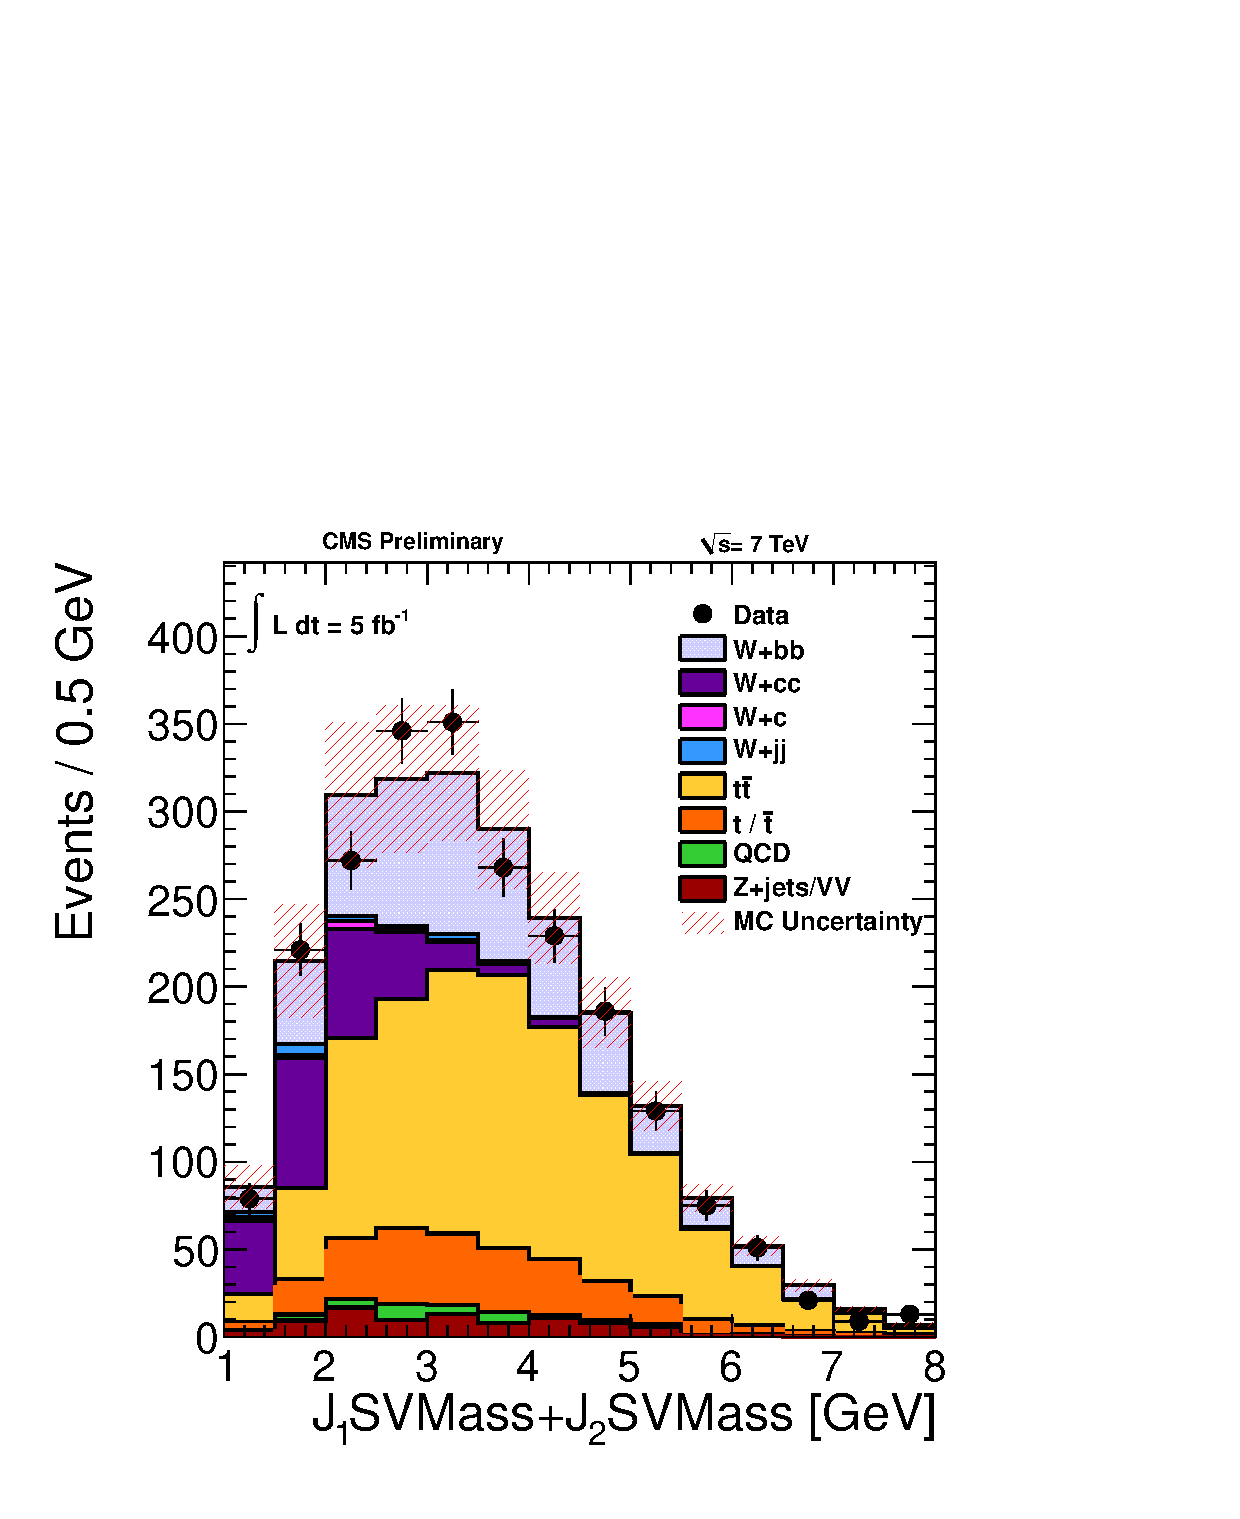
\includegraphics[width=0.45\textwidth]{Wbb/fig3a.pdf}
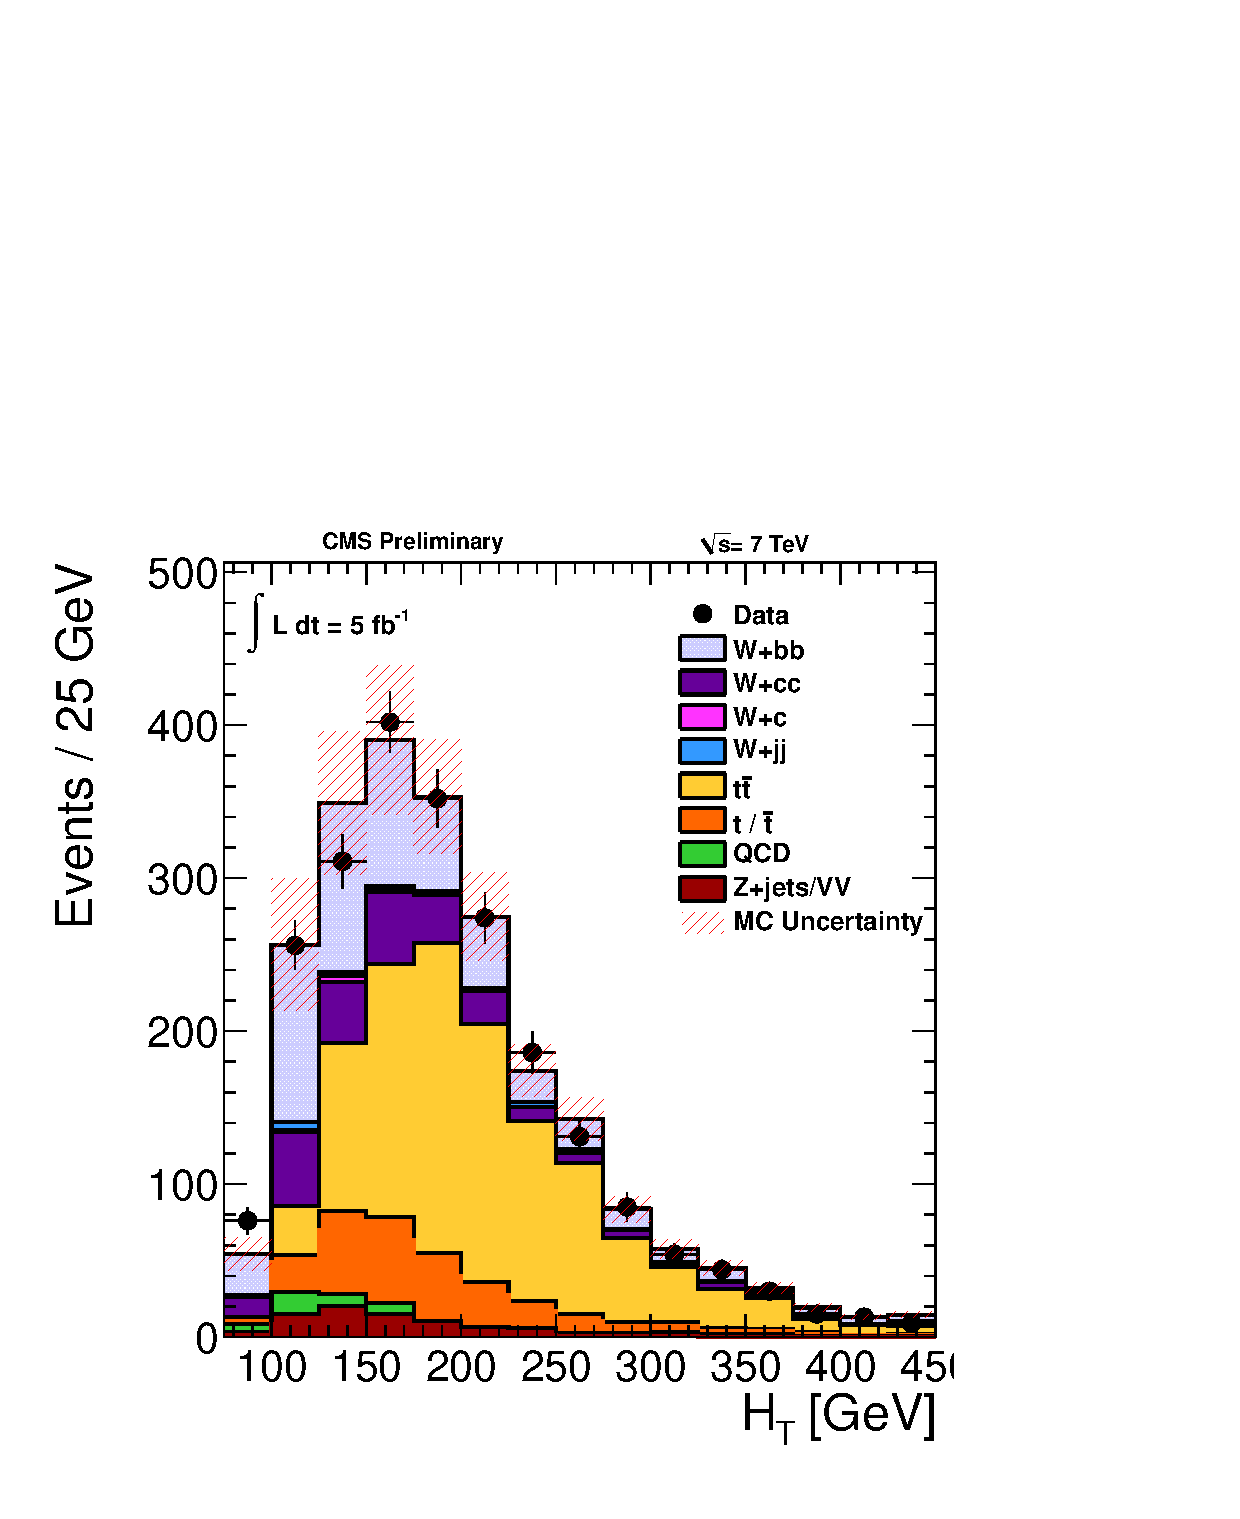
\includegraphics[width=0.45\textwidth]{Wbb/fig4a.pdf}
\caption{
The distribution of the sum of the masses of the two secondary vertices ($\rm{J_1}$ SV mass + $\rm{J_2}$ SV mass) (left)  and $H_{\rm{T}}$ of the system (right) in the alternative
medium b-tag selection, 
normalized to the results of the cross-check fit. 
%To further distinguish between $\Wbb$ and $\Wcc$ we introduce the variable '$J_{1}$ SV mass + $J_{2}$ SV mass',
%this is simply the sum of the invariant masses of the secondary vertex found in each selected jet. (left)
%The distribution of $J_{1}$+$J_{2}$ SV mass in the alternate two medium b-Tag selection is shown with yields after the fit;
%the $J_{1}$+$J_{2}$ SV mass variable provides powerful discrimination of $\Wbb$ and $\Wcc$ in this
%selection where there are looser b-tagging requirements. 
%(right) Distribution of $J_{1}$+$J_{2}$ SV mass in the two tight b-Tag selection.
}
\label{fig:figC}
\end{figure}

\subsection{Final Cross Section Measurement}

The $\Wbb$ cross section within the reference fiducial phase space
is obtained using the expression
\begin{equation*}
\sigma(\Pp\Pp\to \Wbb) \times {\mathcal{B}}(\Wmn)= \frac{N_{S}}{\int{\mathrm{L},t}~\epsilon_{\text{sel}}},
\end{equation*}
where the efficiency of the selection requirements, $\epsilon_{\text{sel}} = (11.2 \pm 1.0)\%$, is computed using the
\MADGRAPH + \PYTHIA MC sample. The uncertainty in this selection efficiency comes from the PDF
and scale variation uncertainties mentioned above.

The fiducial volume is defined by requiring a final-state
muon with $\pt>25$GeV and $|\eta|<2.1$ and exactly two final-state particle jets, reconstructed using the anti-$k_{T}$
jet algorithm with a distance parameter of 0.5, with $\pt>25$GeV and $|\eta|<2.4$ and
with each containing at least one b hadron with $\pt>5$GeV. Events with extra jets are vetoed.
The measured fiducial cross section  is
%\ifthenelse{\boolean{cms@external}}{
\begin{multline*}
\sigma(\Pp\Pp\to \PW + \bbbar) \times {\mathcal{B}}(\Wmn) =0.53\pm  0.05\stat \pm\\
 0.09\syst \pm 0.06\theo \pm 0.01lum pb.
\end{multline*}

%{
%\begin{equation*}
%\sigma(\Pp\Pp\to \PW + \bbbar) \times {\mathcal{B}}(\Wmn) =0.53\pm  0.05\stat \pm 0.09\syst \pm 0.06\theo \pm 0.01lum pb.
%\end{equation*}
%}

This measured value cannot be directly compared to the SM NLO cross section
calculated with $\mathtt{MCFM}$~\cite{Campbell:2010ff, Badger:2010mg} because the latter
pertains to jets of partons, not jets of hadrons, and does not include
the production of $\bbbar$ pairs from double-parton scattering (DPS).

$\mathtt{MCFM}$ predicts a cross section of $0.52 \pm 0.03 pb $ at the parton level,
using the {MSTW2008} NNLO PDF set and setting the factorization
and renormalization scales to $\mu_{\mathrm{F}} = \mu_{\mathrm{R}} = m_{\PW} + 2m_{b}$.
The 0.03 pb uncertainty in the theoretical cross section
is estimated
by varying the scales $\mu_{\mathrm{F}}$, $\mu_{\mathrm{R}}$ simultaneously
up and down by a factor of two. This uncertainty also takes into account the
PDF uncertainties following the PDF4LHC recommendation.
This uncertainty in the theoretical cross section may be underestimated because of
the requirement of exactly two jets in the final state. Therefore, a more conservative
estimate of this uncertainty in the theoretical prediction is computed, following the procedure
described in Ref.~\cite{JetUncertainty}, and the total theoretical uncertainty is found to be 30\%.

Two corrections are needed to link the
theoretical prediction to the  measurement, a hadronization correction and a DPS correction.
At the parton level, the events are required to have a muon of
$\pt > 25GeV$ and $|\eta|<2.1$ and exactly two parton jets of
$\pt > 25GeV$ and $|\eta|<2.4$, each containing a b quark.
The hadronization correction factor $C_{b \to B}=0.92\pm0.01$, calculated using a five-flavor
$\mathtt{MADGRAPH}$ + $\mathtt{PYTHIA}$ reference MC, is used to extrapolate the cross section computed
at the level of parton jets to the level of final-state particle jets.
The uncertainty assigned to this correction
is obtained by comparing the corresponding factors computed with a four-flavored $\mathtt{MADGRAPH}$ MC simulation.
The simulated $\mathtt{MADGRAPH}$ + $\mathtt{PYTHIA}$ events include DPS
production of $\bbbar$ pairs and they reproduce these processes adequately
as measured by CMS~\cite{CMS_DPS}. The contribution of DPS events to the cross section
at the parton-jet level is estimated to be $\sigma_{\mathrm{DPS}} = (\sigma_{\PW} \times \sigma_{\bbbar})/\sigma_{\text{eff}}=0.08\pm0.05 pb$.
The value of the effective cross section, $\sigma_{\text{eff}}$, is taken from Ref.~\cite{ATLAS_DPS},
and is assumed to be independent of the process and interaction scale.
The uncertainty in $\sigma_{\mathrm{DPS}}$ takes into account both the uncertainty in the measurement of $\sigma_{\text{eff}}$
and the uncertainty in the fiducial $\bbbar$ cross section.
The theoretical cross section at hadron level can be extrapolated from the $\mathtt{MCFM}$ parton-jet prediction by applying the hadronization correction and
adding the DPS contribution,
resulting in $0.55 \pm0.03(MCFM) \pm 0.01(had)  \pm 0.05(DPS) pb$.
This value is in agreement with the measured value.

\subsection{Additional $\Wbb$ Kinematic Distributions}
\begin{figure}
\centering
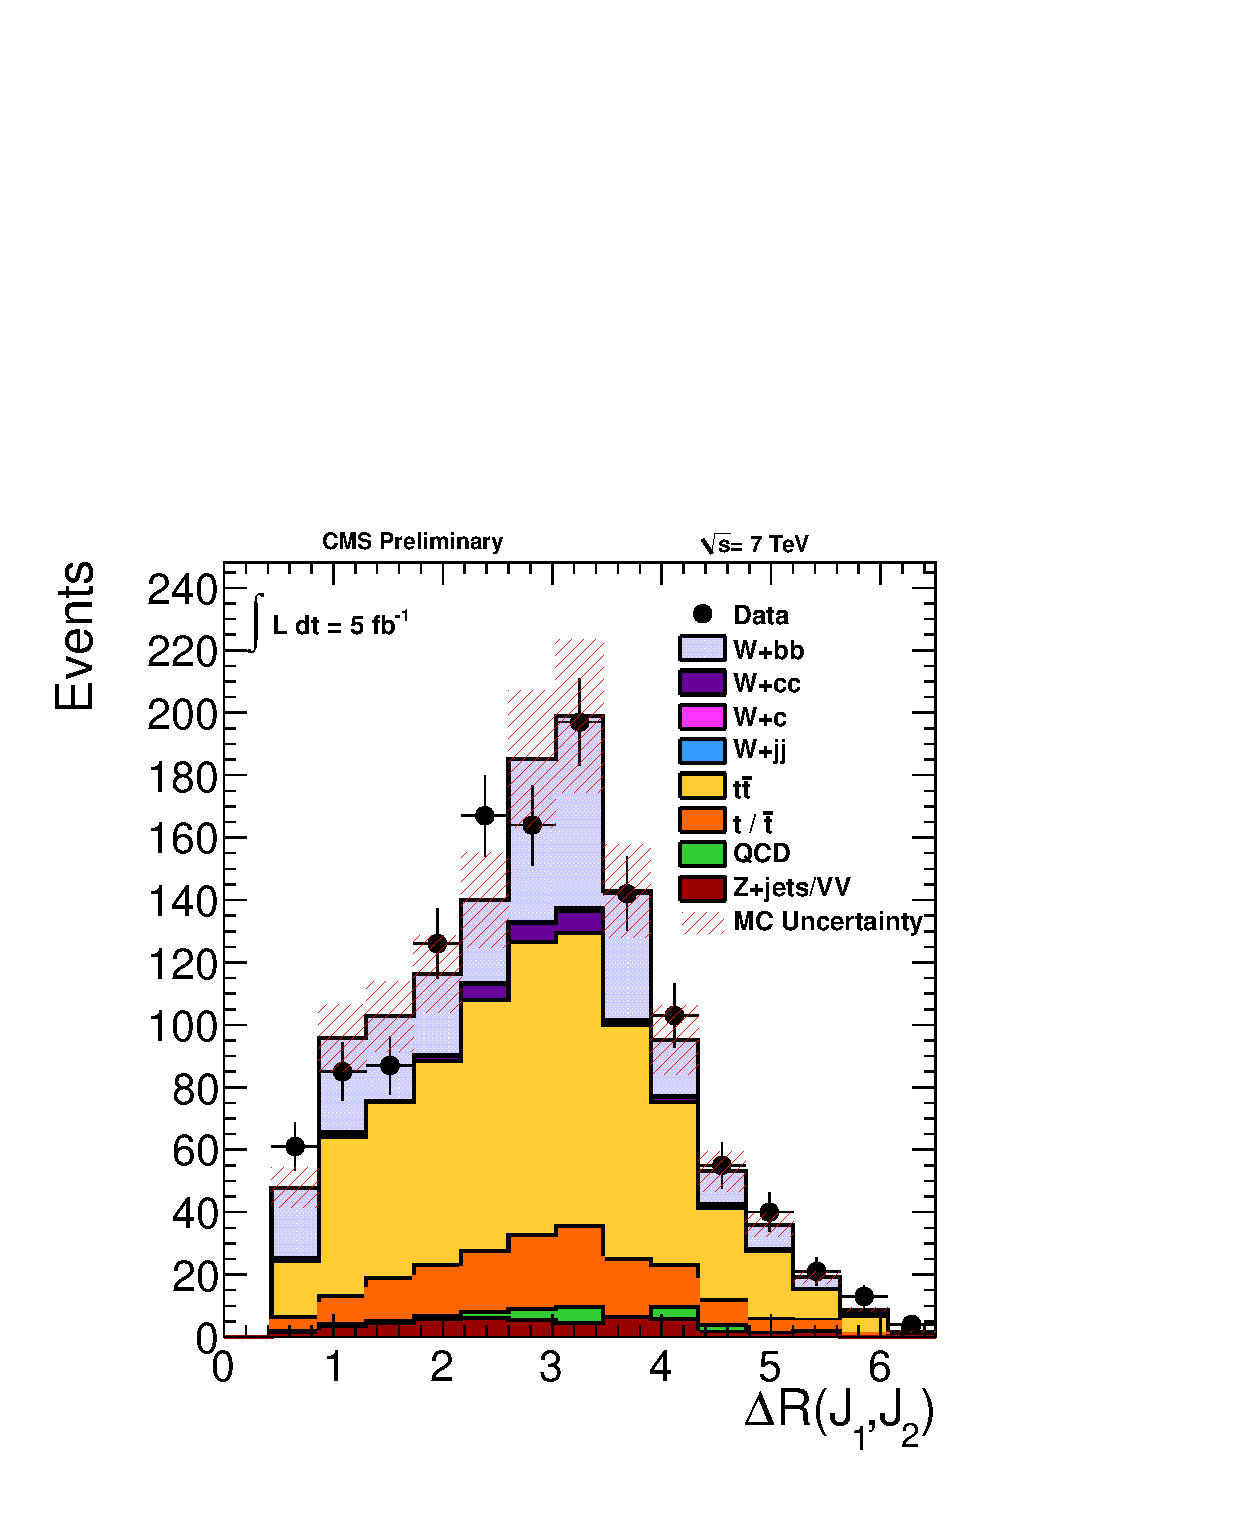
\includegraphics[width=0.45\textwidth]{Wbb/fig5.pdf}
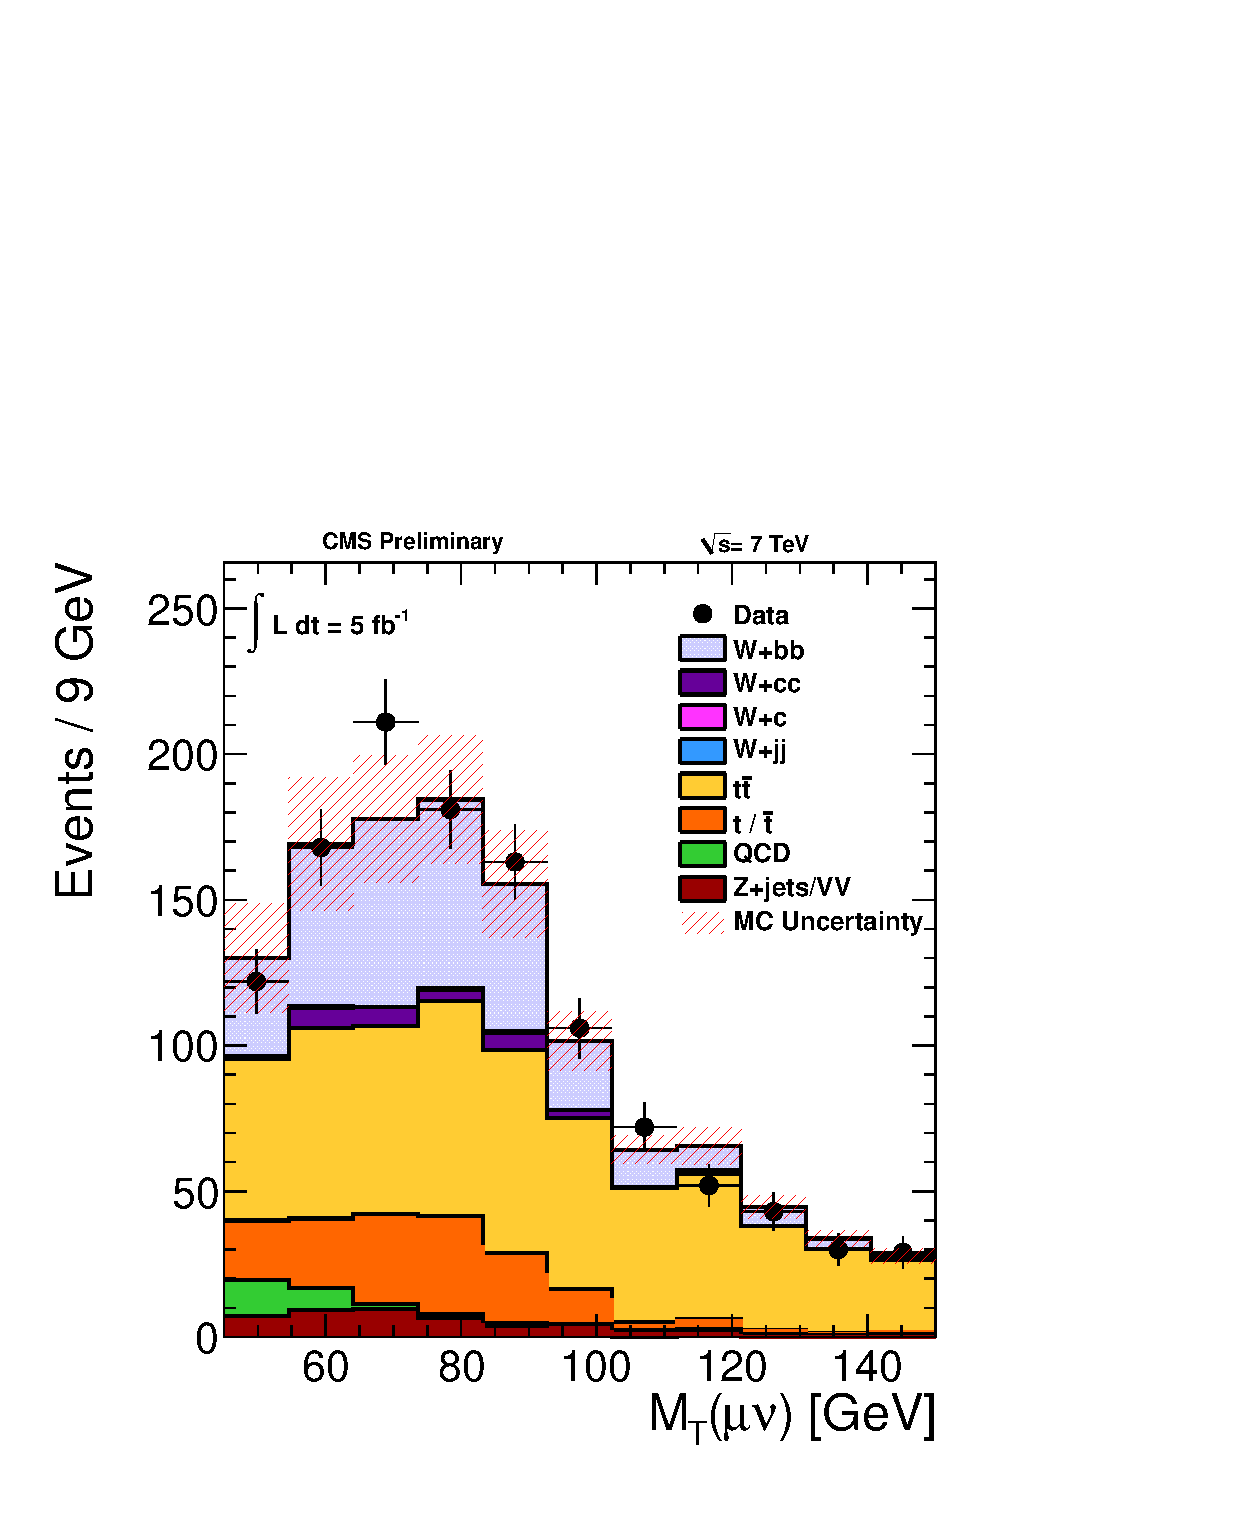
\includegraphics[width=0.45\textwidth]{Wbb/fig6.pdf}
\caption{(left) The $\Delta R$ between the two selected b jets
(right) the $\MT$ distribution, normalized to the results of the fit.}
\label{fig:figD}
\end{figure}

In addition to this measurement of the cross section, we have explored the kinematics of the $\Wbb$ system.
The angular distance between two selected b jets, $\Delta R(\rm{J_1,J_2})$ 
and the $\MT$ distribution are compared to Monte Carlo predictions 
in Fig.~\ref{fig:figD}. The shapes are taken from simulation and are normalized to the fit results. 
Figure~\ref{fig:figE} shows the invariant mass of the two 
selected b jets system and its $\pt$.
The observed distributions  are well described by the simulation.
%Those distributions are very important for the dominant background background estimation
%in the $WH\rightarrow l \nu b \bar{b}$ search.


%The measured cross section, unfolded to the b-hadron level as described above, for muons with
%$\pt > 25GeV$ and $|\eta|<2.1$ and two b-jets with
%$\pt > 25GeV$ and $|\eta|<2.4$ is found to be 
%$1.17\pm  0.10\stat ^{+0.21}_{-0.17}\syst \pm 0.09 \theo \pm 0.03\lumi \unit{pb.}$

% No quoting MCFM until we fix the C(parton, hadron) factor

%In summary, we have presented a measurement of the $\Wbb$ production
%cross section in proton-proton collisions at 7\TeV. The W+$\bbbar$ events
%have been  selected in the W $\to \mu\nu$ decay mode with a 
%muon of $\pt>25GeV$ and $|\eta|<2.1$, and two b jets with $\pt>25GeV$ and $|\eta|<2.4$. 
%The data sample corresponds to an integrated luminosity of $5.0\fbinv$.
%%The measured cross section
%%$\sigma ( \Wbb) =  0.98 \pm 0.12 \stat \pm0.20 \syst \pm 0.07 \theo \pm 0.02\lumi pb.$
%%is consistent with the SM prediction.
%The measured cross section 
%%$\sigma ( \Wbb) =  0.98 \pm 0.12 \stat \pm0.20 \syst \pm 0.07 \theo \pm 0.02\lumi \unit{pb}$
%%$\sigma ( \Wbb) = 1.17\pm  0.10\stat ^{+0.21}_{-0.17}\syst \pm 0.18 \theo \pm 0.03\lumi \unit{pb.}$
%$\sigma(pp\rightarrow \mathrm{W} + \bbbar, p_T^{\mathrm{b}}>25~GeV, |\eta^{\mathrm{b}}|<2.4)\times {\cal{B}}(\Wmn, p_T^{\mu}>25~GeV, |\eta^{\mu}|<2.1) =0.53\pm  0.05\stat \pm 0.09 \syst \pm 0.06 \theo \pm 0.01\lumi pb.$
%for production of a W boson in association with two b jets is in agreement with
%the SM predictions.
%This result is approaching the precision of theoretical predictions at NNLO, 
%allowing a sensitive test of perturbative calculations
%in the SM.


\begin{figure}
\centering
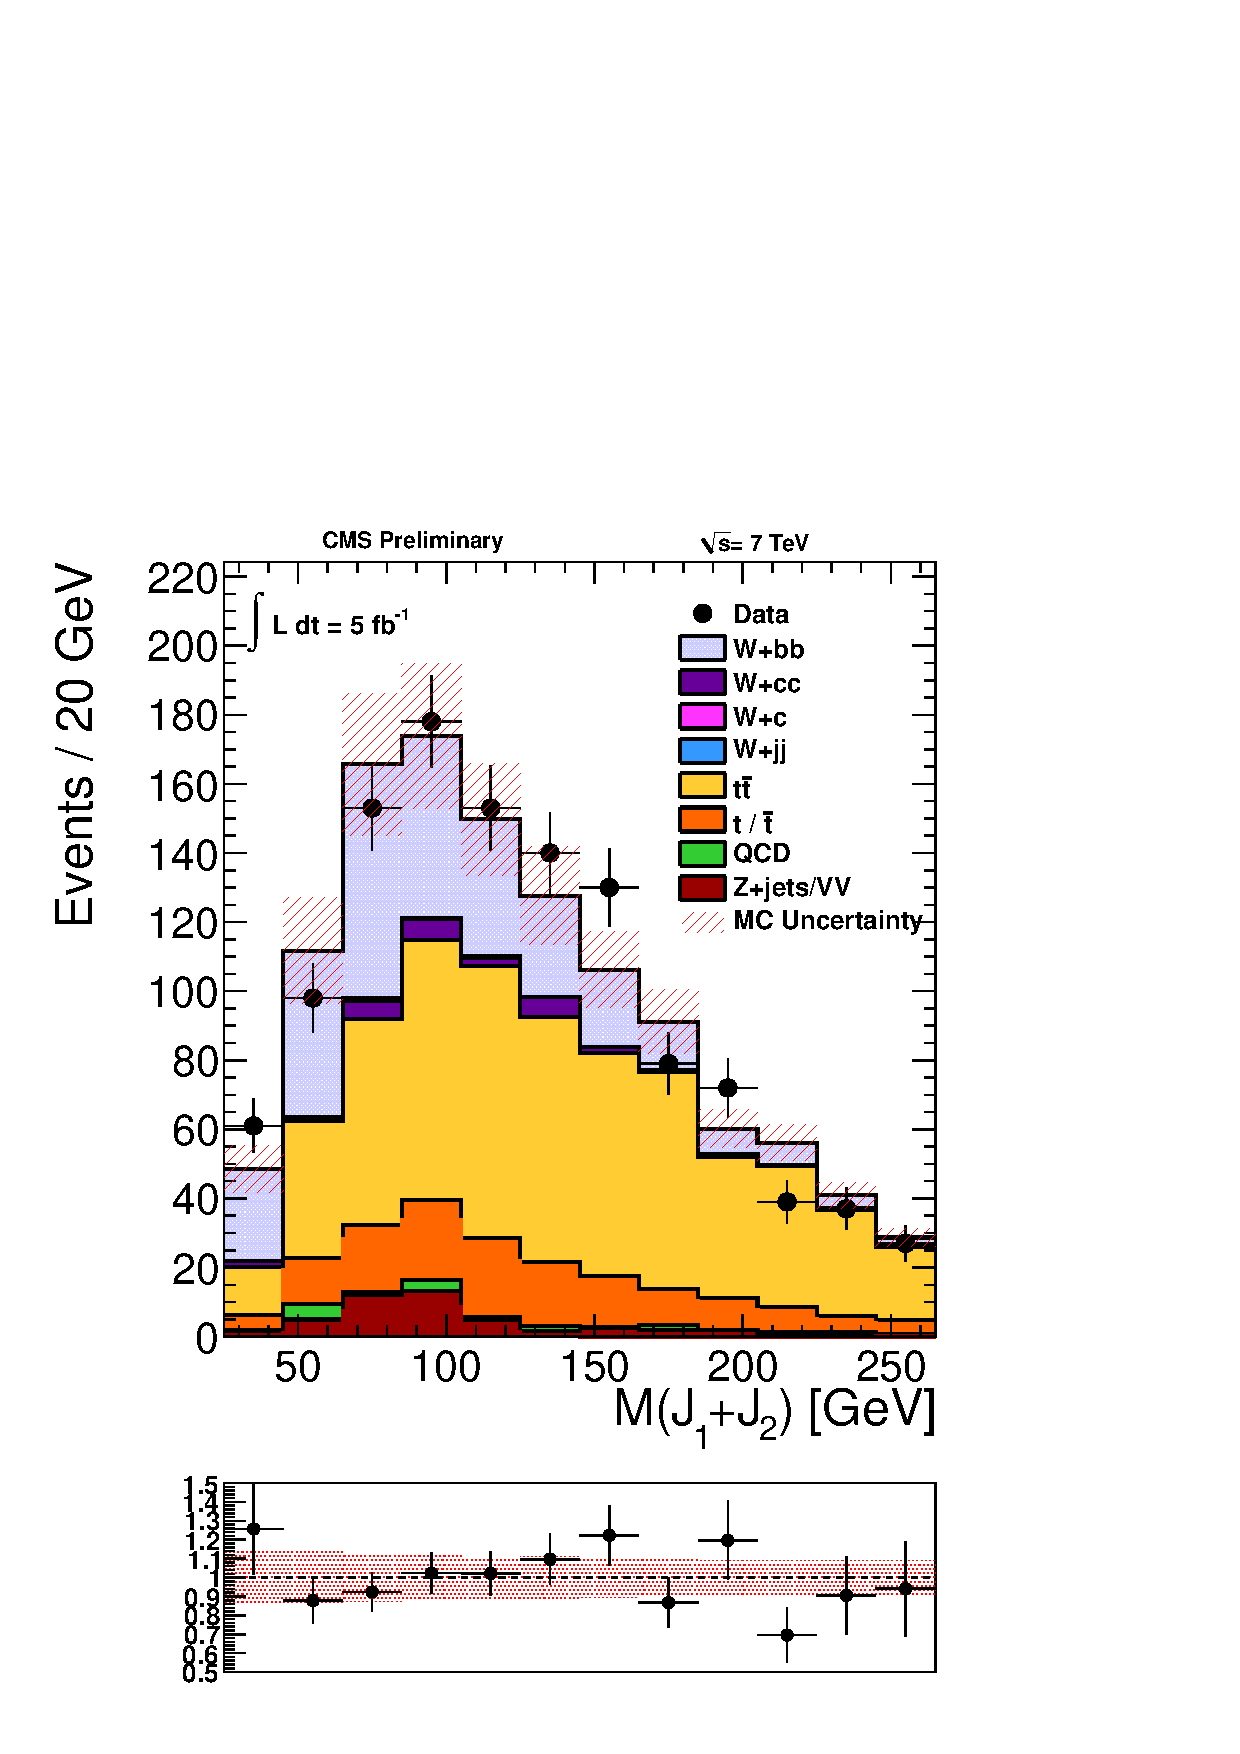
\includegraphics[width=0.45\textwidth, trim = 0 4cm 0 0, clip=true ]{Wbb/fig7.pdf}
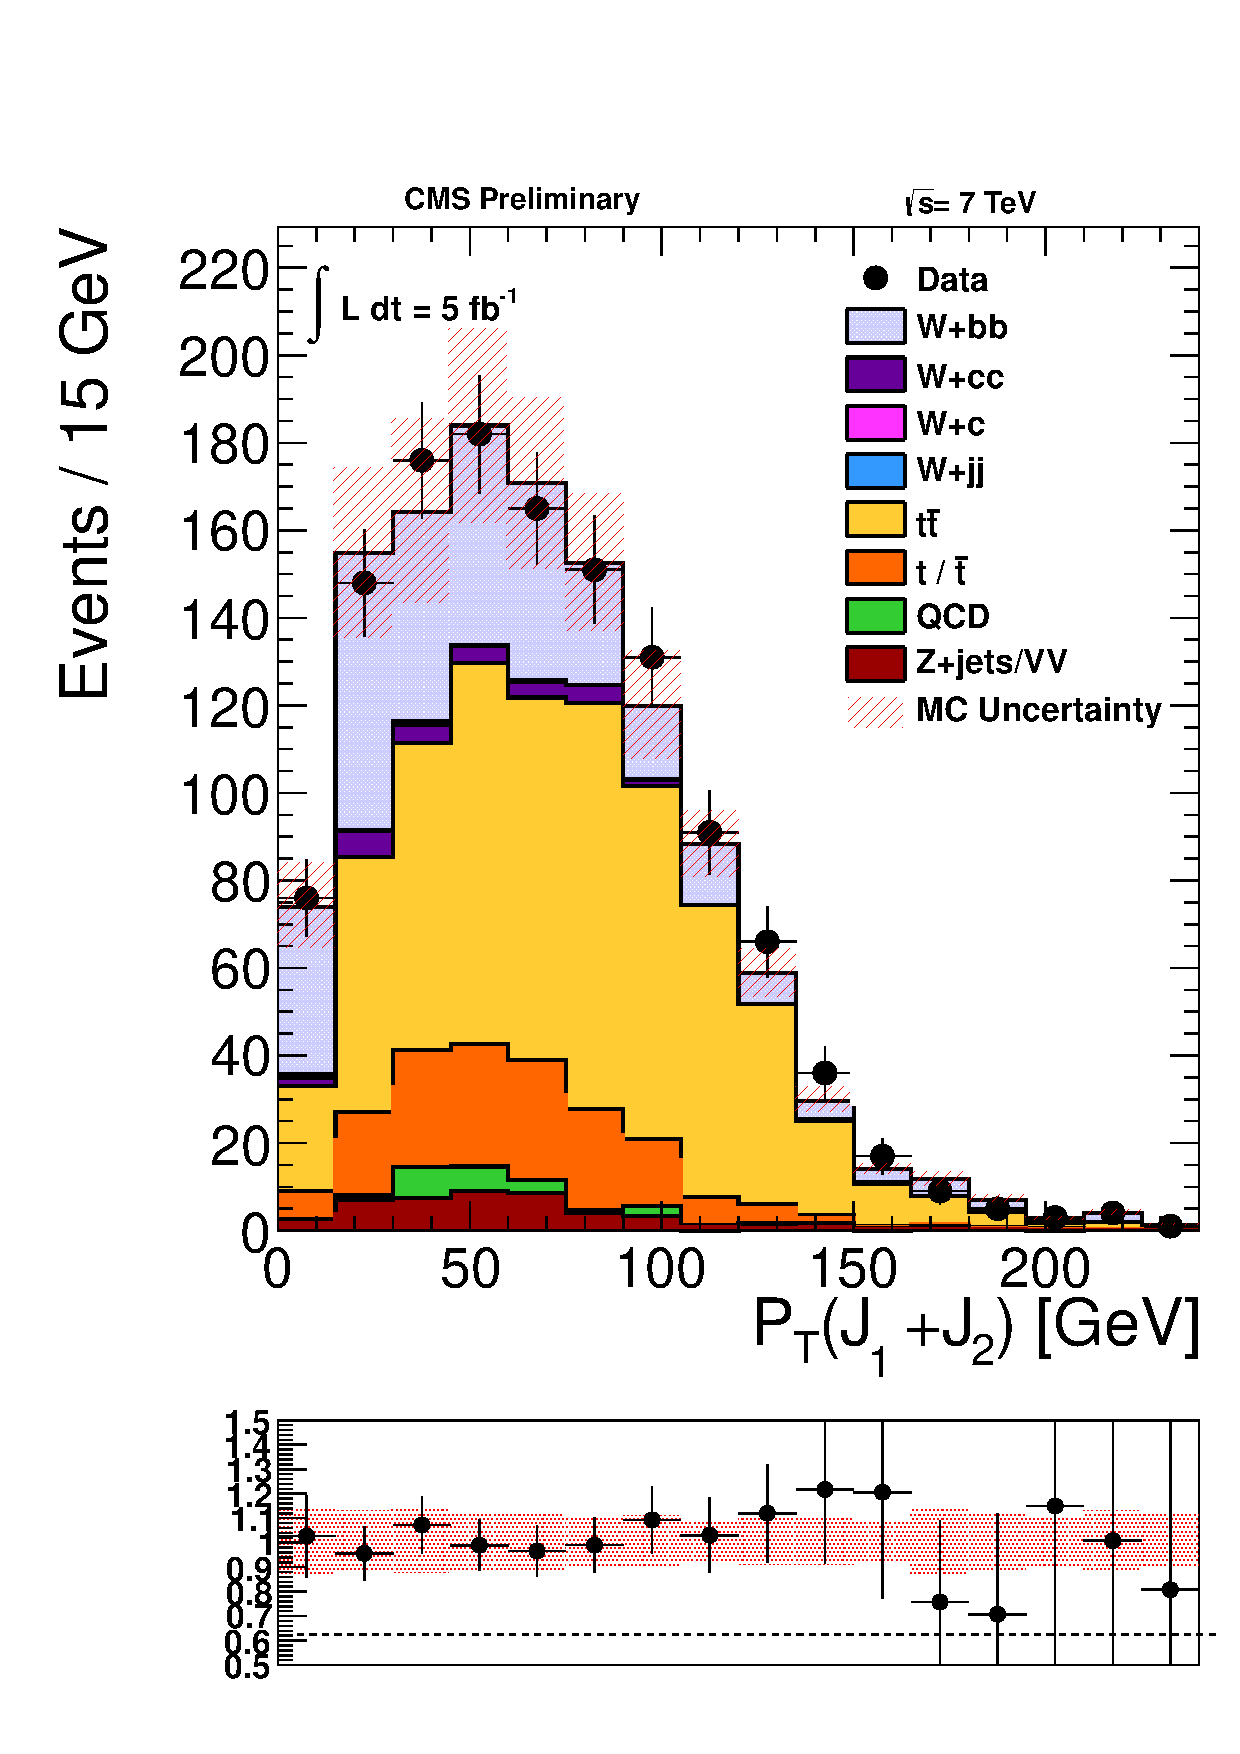
\includegraphics[width=0.45\textwidth, trim = 0 5cm 0 0, clip=true ]{Wbb/fig8.pdf}
\caption{(left) The invariant mass, $m_{\rm{J_{1} J_{2}}}$ of the two selected b jets and 
(right) the $p_{T}(J_{1} J_{2})$ distribution, normalized to the results of the fit.}
\label{fig:figE}
\end{figure}
